\documentclass[twoside]{book}

% Packages required by doxygen
\usepackage{calc}
\usepackage{doxygen}
\usepackage{graphicx}
\usepackage[utf8]{inputenc}
\usepackage{makeidx}
\usepackage{multicol}
\usepackage{multirow}
\usepackage{textcomp}
\usepackage[table]{xcolor}

% Font selection
\usepackage[T1]{fontenc}
\usepackage{mathptmx}
\usepackage[scaled=.90]{helvet}
\usepackage{courier}
\usepackage{amssymb}
\usepackage{sectsty}
\renewcommand{\familydefault}{\sfdefault}
\allsectionsfont{%
  \fontseries{bc}\selectfont%
  \color{darkgray}%
}
\renewcommand{\DoxyLabelFont}{%
  \fontseries{bc}\selectfont%
  \color{darkgray}%
}

% Page & text layout
\usepackage{geometry}
\geometry{%
  a4paper,%
  top=2.5cm,%
  bottom=2.5cm,%
  left=2.5cm,%
  right=2.5cm%
}
\tolerance=750
\hfuzz=15pt
\hbadness=750
\setlength{\emergencystretch}{15pt}
\setlength{\parindent}{0cm}
\setlength{\parskip}{0.2cm}
\makeatletter
\renewcommand{\paragraph}{%
  \@startsection{paragraph}{4}{0ex}{-1.0ex}{1.0ex}{%
    \normalfont\normalsize\bfseries\SS@parafont%
  }%
}
\renewcommand{\subparagraph}{%
  \@startsection{subparagraph}{5}{0ex}{-1.0ex}{1.0ex}{%
    \normalfont\normalsize\bfseries\SS@subparafont%
  }%
}
\makeatother

% Headers & footers
\usepackage{fancyhdr}
\pagestyle{fancyplain}
\fancyhead[LE]{\fancyplain{}{\bfseries\thepage}}
\fancyhead[CE]{\fancyplain{}{}}
\fancyhead[RE]{\fancyplain{}{\bfseries\leftmark}}
\fancyhead[LO]{\fancyplain{}{\bfseries\rightmark}}
\fancyhead[CO]{\fancyplain{}{}}
\fancyhead[RO]{\fancyplain{}{\bfseries\thepage}}
\fancyfoot[LE]{\fancyplain{}{}}
\fancyfoot[CE]{\fancyplain{}{}}
\fancyfoot[RE]{\fancyplain{}{\bfseries\scriptsize Generated on Sun Jan 12 2014 16\-:36\-:27 for Chase game by Doxygen }}
\fancyfoot[LO]{\fancyplain{}{\bfseries\scriptsize Generated on Sun Jan 12 2014 16\-:36\-:27 for Chase game by Doxygen }}
\fancyfoot[CO]{\fancyplain{}{}}
\fancyfoot[RO]{\fancyplain{}{}}
\renewcommand{\footrulewidth}{0.4pt}
\renewcommand{\chaptermark}[1]{%
  \markboth{#1}{}%
}
\renewcommand{\sectionmark}[1]{%
  \markright{\thesection\ #1}%
}

% Indices & bibliography
\usepackage{natbib}
\usepackage[titles]{tocloft}
\setcounter{tocdepth}{3}
\setcounter{secnumdepth}{5}
\makeindex

% Hyperlinks (required, but should be loaded last)
\usepackage{ifpdf}
\ifpdf
  \usepackage[pdftex,pagebackref=true]{hyperref}
\else
  \usepackage[ps2pdf,pagebackref=true]{hyperref}
\fi
\hypersetup{%
  colorlinks=true,%
  linkcolor=blue,%
  citecolor=blue,%
  unicode%
}

% Custom commands
\newcommand{\clearemptydoublepage}{%
  \newpage{\pagestyle{empty}\cleardoublepage}%
}


%===== C O N T E N T S =====

\begin{document}

% Titlepage & ToC
\hypersetup{pageanchor=false}
\pagenumbering{roman}
\begin{titlepage}
\vspace*{7cm}
\begin{center}%
{\Large Chase game \\[1ex]\large 1 }\\
\vspace*{1cm}
{\large Generated by Doxygen 1.8.6}\\
\vspace*{0.5cm}
{\small Sun Jan 12 2014 16:36:27}\\
\end{center}
\end{titlepage}
\clearemptydoublepage
\tableofcontents
\clearemptydoublepage
\pagenumbering{arabic}
\hypersetup{pageanchor=true}

%--- Begin generated contents ---
\chapter{Main Page}
\label{index}\hypertarget{index}{}Modified catch me if you can game Remastered by your group with new rules.

The game plays in \char`\"{}real time\char`\"{}, the objective is for one player is to catch the other and is for the other player to not being caught.

Keys are configurable in .mapconfig Maps options are configurable in .gameconfig 
\chapter{(F\-R) A\-J\-O\-U\-T\-S P\-A\-R R\-A\-P\-P\-O\-R\-T A\-U S\-U\-J\-E\-T}
\label{md__c_h_a_n_g_e_s}
\hypertarget{md__c_h_a_n_g_e_s}{}
\subsection*{Changements }

Les changements que nous avons apporté au jeu original.

Nous avons ajouté des structures compreneant l'ensemble des paramètres du jeu afin d'aiser le code. Par exemple, nous avons rajouté une structure S\-Game\-Status qui va contenir l'ensemble de l'état la configuration du jeu, comme le numéro de la manche actuelle, la position des players et les code de touches à utiliser pour bouger les playrs. La configuration de gamestatus peut être chargée depuis le fichier .gameconfig. Le jeu va ensuite se charger lui même d'initialiser le jeu correctement en appliquant les paramètres.

Nous avons changé la génération de la carte en ajoutant un générateur d'obstacles aléatoires, générant des formes dont le nombre varia en fonction du niveau de difficulté (choisi aléatoirement par le jeu).

Nous avons ajouté de la musique, avec l'utilisation de la librairie S\-F\-M\-L, en particulier sa partie audio pour charger et jouer des fichiers sonores. La musique à la particularité d'être dynamique \-: elle va changer en fonction de l'état du jeu. (chagnement de volume des pistes sonores).

Nous avons ajouté un système de bonus et de malus, permettant de rajouter un peu de sauce piquante au jeu.

Nous avons ajouté un écran titre et quelques menus afin que le joueur soit plus à l'aise lors du lancement du jeu et commprenne ce qu'il doit faire.

Nous avons chagné fondamentalement le principe et les règles du jeu \-: Un joueur doit chasser l'autre tour à tour et le jeu se joue en temps réel. Par exemple, au premier round, c'est le joueur 1 qui doit chasser le joueur 2, et inversement pour chque round. Le terme \char`\"{}temps réel\char`\"{} signifie que les joueurs peuvent jouer en même temps, en appuyant au clavier en même temps pour rendre le jeu plus frénétique. Les joueurs peuvent donc envoyer leur input {\itshape en même temps}, à condition qu'ils martèlent leur clavier (ne par resté enfoncé sur un bouton).

\subsection*{Méthode de test et de travail }

Afin de tester les nouvelles fonctionalités alors que le jeu n'était pas terminé, nous nous étions basés sur un moteur simple (le code de base), en y rajoutant notre code et testant si il fonctionnait bien.

Nous avons aussi utilisé G\-I\-T pour gérere les différentes versions du programme et créer quelques branches quand on voulait implémenter une fonctionnalité qui pouvait causer des problèmes.

Ainsi (et aussi grâce à la séparation en plusieurs fichiers), nous avons pu nous partager plus facilement le travail. 
\chapter{R\-E\-A\-D\-M\-E}
\label{md__r_e_a_d_m_e}
\hypertarget{md__r_e_a_d_m_e}{}
You need to install S\-F\-M\-L 1.\-6 lib to be able to compile. Exemple of installation command for ubuntu 13.\-10 \-: sudo apt-\/get install mesa-\/common-\/dev ibglu-\/dev sudo apt-\/get libsfml-\/dev

\section*{S\-O\-U\-N\-D C\-R\-E\-D\-I\-T}

Validation sound effect by broumbroum, under a creative commons 3.\-0 by licence \href{http://www.freesound.org/people/broumbroum/sounds/50565/}{\tt http\-://www.\-freesound.\-org/people/broumbroum/sounds/50565/}

Game music is \char`\"{}\-Trickyness\char`\"{} under C\-C B\-Y licence by Josua Gonzalez 
\chapter{Namespace Index}
\section{Namespace List}
Here is a list of all namespaces with brief descriptions\-:\begin{DoxyCompactList}
\item\contentsline{section}{\hyperlink{namespace_chase_game}{Chase\-Game} }{\pageref{namespace_chase_game}}{}
\end{DoxyCompactList}

\chapter{Class Index}
\section{Class List}
Here are the classes, structs, unions and interfaces with brief descriptions\-:\begin{DoxyCompactList}
\item\contentsline{section}{\hyperlink{struct_chase_game_1_1_s_color_set}{Chase\-Game\-::\-S\-Color\-Set} \\*Color set to use when displaying the map }{\pageref{struct_chase_game_1_1_s_color_set}}{}
\item\contentsline{section}{\hyperlink{struct_chase_game_1_1_s_game_status}{Chase\-Game\-::\-S\-Game\-Status} \\*Contains game configuration }{\pageref{struct_chase_game_1_1_s_game_status}}{}
\item\contentsline{section}{\hyperlink{struct_chase_game_1_1_s_map_gen_params}{Chase\-Game\-::\-S\-Map\-Gen\-Params} \\*Contains all the map generation parameters }{\pageref{struct_chase_game_1_1_s_map_gen_params}}{}
\item\contentsline{section}{\hyperlink{struct_chase_game_1_1_s_player_keys}{Chase\-Game\-::\-S\-Player\-Keys} \\*Player specific keys }{\pageref{struct_chase_game_1_1_s_player_keys}}{}
\item\contentsline{section}{\hyperlink{struct_chase_game_1_1_s_player_pos}{Chase\-Game\-::\-S\-Player\-Pos} \\*Defines a position }{\pageref{struct_chase_game_1_1_s_player_pos}}{}
\item\contentsline{section}{\hyperlink{struct_chase_game_1_1_s_player_state}{Chase\-Game\-::\-S\-Player\-State} \\*Player state }{\pageref{struct_chase_game_1_1_s_player_state}}{}
\end{DoxyCompactList}

\chapter{File Index}
\section{File List}
Here is a list of all files with brief descriptions\-:\begin{DoxyCompactList}
\item\contentsline{section}{\hyperlink{audio_8cxx}{audio.\-cxx} }{\pageref{audio_8cxx}}{}
\item\contentsline{section}{\hyperlink{audio_8hxx}{audio.\-hxx} \\*\hyperlink{audio_8cxx}{Audio.\-cxx} function prototypes }{\pageref{audio_8hxx}}{}
\item\contentsline{section}{\hyperlink{banana_8cxx}{banana.\-cxx} \\*Super Banana ! }{\pageref{banana_8cxx}}{}
\item\contentsline{section}{\hyperlink{banana_8hxx}{banana.\-hxx} \\*\hyperlink{banana_8cxx}{Banana.\-cxx} function prototypes }{\pageref{banana_8hxx}}{}
\item\contentsline{section}{\hyperlink{bonus_8cxx}{bonus.\-cxx} \\*File related bonus and malus }{\pageref{bonus_8cxx}}{}
\item\contentsline{section}{\hyperlink{bonus_8hxx}{bonus.\-hxx} \\*\hyperlink{bonus_8cxx}{Bonus.\-cxx} function prototypes }{\pageref{bonus_8hxx}}{}
\item\contentsline{section}{\hyperlink{file_8cxx}{file.\-cxx} \\*File related functions }{\pageref{file_8cxx}}{}
\item\contentsline{section}{\hyperlink{file_8hxx}{file.\-hxx} \\*\hyperlink{file_8cxx}{File.\-cxx} function prototypes }{\pageref{file_8hxx}}{}
\item\contentsline{section}{\hyperlink{game_8cxx}{game.\-cxx} \\*Audio related functions }{\pageref{game_8cxx}}{}
\item\contentsline{section}{\hyperlink{game_8hxx}{game.\-hxx} \\*\hyperlink{game_8cxx}{Game.\-cxx} function prototypes }{\pageref{game_8hxx}}{}
\item\contentsline{section}{\hyperlink{globals_8hxx}{globals.\-hxx} \\*Defines global constants and variables for the \hyperlink{namespace_chase_game}{Chase\-Game} namespace }{\pageref{globals_8hxx}}{}
\item\contentsline{section}{\hyperlink{main_8cxx}{main.\-cxx} \\*Main file }{\pageref{main_8cxx}}{}
\item\contentsline{section}{\hyperlink{map_8cxx}{map.\-cxx} \\*Map related function }{\pageref{map_8cxx}}{}
\item\contentsline{section}{\hyperlink{map_8hxx}{map.\-hxx} \\*\hyperlink{map_8cxx}{Map.\-cxx} function prototypes }{\pageref{map_8hxx}}{}
\item\contentsline{section}{\hyperlink{unix_8cxx}{unix.\-cxx} \\*Defines unix-\/only functions }{\pageref{unix_8cxx}}{}
\item\contentsline{section}{\hyperlink{unix_8hxx}{unix.\-hxx} \\*\hyperlink{unix_8cxx}{Unix.\-cxx} function prototypes }{\pageref{unix_8hxx}}{}
\end{DoxyCompactList}

\chapter{Namespace Documentation}
\hypertarget{namespace_chase_game}{\section{Chase\-Game Namespace Reference}
\label{namespace_chase_game}\index{Chase\-Game@{Chase\-Game}}
}
\subsection*{Classes}
\begin{DoxyCompactItemize}
\item 
struct \hyperlink{struct_chase_game_1_1_s_player_pos}{S\-Player\-Pos}
\begin{DoxyCompactList}\small\item\em Defines a position. \end{DoxyCompactList}\item 
struct \hyperlink{struct_chase_game_1_1_s_map_gen_params}{S\-Map\-Gen\-Params}
\begin{DoxyCompactList}\small\item\em Contains all the map generation parameters. \end{DoxyCompactList}\item 
struct \hyperlink{struct_chase_game_1_1_s_player_keys}{S\-Player\-Keys}
\begin{DoxyCompactList}\small\item\em Player specific keys. \end{DoxyCompactList}\item 
struct \hyperlink{struct_chase_game_1_1_s_player_state}{S\-Player\-State}
\begin{DoxyCompactList}\small\item\em Player state. \end{DoxyCompactList}\item 
struct \hyperlink{struct_chase_game_1_1_s_color_set}{S\-Color\-Set}
\begin{DoxyCompactList}\small\item\em Color set to use when displaying the map. \end{DoxyCompactList}\item 
struct \hyperlink{struct_chase_game_1_1_s_game_status}{S\-Game\-Status}
\begin{DoxyCompactList}\small\item\em Contains game configuration. \end{DoxyCompactList}\end{DoxyCompactItemize}
\subsection*{Typedefs}
\begin{DoxyCompactItemize}
\item 
typedef std\-::vector$<$ char $>$ \hyperlink{namespace_chase_game_aa09cf1806d3b1f59d36cfabadeaca6a2}{C\-V\-Line}
\begin{DoxyCompactList}\small\item\em Matrix line type. \end{DoxyCompactList}\item 
typedef std\-::vector$<$ \hyperlink{namespace_chase_game_aa09cf1806d3b1f59d36cfabadeaca6a2}{C\-V\-Line} $>$ \hyperlink{namespace_chase_game_a469449f9237e59efce3982127366c550}{C\-Matrix}
\begin{DoxyCompactList}\small\item\em Matrix type. \end{DoxyCompactList}\end{DoxyCompactItemize}
\subsection*{Enumerations}
\begin{DoxyCompactItemize}
\item 
enum \hyperlink{namespace_chase_game_a2501a45afa3eb11b10e04d79a8349796}{Langs} \{ \hyperlink{namespace_chase_game_a2501a45afa3eb11b10e04d79a8349796a4259ad53ebc5f91f2615cf5a5f59bece}{L\-A\-N\-G\-\_\-\-F\-R}, 
\hyperlink{namespace_chase_game_a2501a45afa3eb11b10e04d79a8349796a8d86c92b659a6ebac045d0a20e3fba0d}{L\-A\-N\-G\-\_\-\-E\-N}, 
\hyperlink{namespace_chase_game_a2501a45afa3eb11b10e04d79a8349796a2458ded06b17611b5fb00d6a095a4dd2}{L\-A\-N\-G\-\_\-\-E\-S}
 \}
\begin{DoxyCompactList}\small\item\em Language codes. \end{DoxyCompactList}\item 
enum \hyperlink{namespace_chase_game_a5d785ea23167a3b7e44e045097cd457e}{Difficulty\-Levels} \{ \hyperlink{namespace_chase_game_a5d785ea23167a3b7e44e045097cd457ea8511737cb33e0a6022084ed1b5c05092}{D\-I\-F\-F\-L\-V\-L\-\_\-\-E\-A\-S\-Y}, 
\hyperlink{namespace_chase_game_a5d785ea23167a3b7e44e045097cd457ea124bdf49731fecdaa92d39fbd9d98f26}{D\-I\-F\-F\-L\-V\-L\-\_\-\-N\-O\-R\-M}, 
\hyperlink{namespace_chase_game_a5d785ea23167a3b7e44e045097cd457ea67fccff53bbaeaa47737530842f5c4f5}{D\-I\-F\-F\-L\-V\-L\-\_\-\-H\-A\-R\-D}, 
\hyperlink{namespace_chase_game_a5d785ea23167a3b7e44e045097cd457ea6c71b45deb89801d0e11e674d21e3e51}{D\-I\-F\-F\-L\-V\-L\-\_\-\-C\-R\-Z\-Y}
 \}
\begin{DoxyCompactList}\small\item\em Difficulty levels. \end{DoxyCompactList}\end{DoxyCompactItemize}
\subsection*{Functions}
\begin{DoxyCompactItemize}
\item 
\hyperlink{struct_chase_game_1_1_s_map_gen_params}{S\-Map\-Gen\-Params} \hyperlink{namespace_chase_game_a4779af792d3de8e274049bf2019e0343}{Load\-Map\-Gen\-Config} (const string \&File\-Name)
\item 
bool \hyperlink{namespace_chase_game_a98e8d90127c802c1445266e39966c3fb}{Save\-Map\-Config} (const string \&File\-Name, \hyperlink{struct_chase_game_1_1_s_map_gen_params}{S\-Map\-Gen\-Params} \&Params)
\item 
\hyperlink{struct_chase_game_1_1_s_game_status}{S\-Game\-Status} \hyperlink{namespace_chase_game_addd460052ec5a5fe3010665ca84b07ec}{Load\-Game\-Config} (const std\-::string \&File\-Name)
\begin{DoxyCompactList}\small\item\em Loads game configuration. \end{DoxyCompactList}\item 
bool \hyperlink{namespace_chase_game_a39f8b039151b1a3eef82fdc1c6f52091}{Save\-Game\-Config} (const string \&File\-Name, \hyperlink{struct_chase_game_1_1_s_game_status}{S\-Game\-Status} \&Config)
\item 
\hyperlink{struct_chase_game_1_1_s_map_gen_params}{S\-Map\-Gen\-Params} \hyperlink{namespace_chase_game_a9c5b5d91cb4251cae461faa4ace8a0cf}{Load\-Map\-Gen\-Config} (const std\-::string \&File\-Name)
\begin{DoxyCompactList}\small\item\em Loads parameters from a config file. \end{DoxyCompactList}\item 
bool \hyperlink{namespace_chase_game_a4c62f61c6aac5bf06292aa51294fd211}{Save\-Map\-Config} (const std\-::string \&File\-Name, \hyperlink{struct_chase_game_1_1_s_map_gen_params}{S\-Map\-Gen\-Params} \&Params)
\begin{DoxyCompactList}\small\item\em Saves parameters in a config file. \end{DoxyCompactList}\item 
bool \hyperlink{namespace_chase_game_a561c85a018e34c8baa21f7f500a3c9c7}{Save\-Game\-Config} (const std\-::string \&File\-Name, \hyperlink{struct_chase_game_1_1_s_game_status}{S\-Game\-Status} \&Config)
\begin{DoxyCompactList}\small\item\em Saves game configuration in a config file. \end{DoxyCompactList}\item 
char \hyperlink{namespace_chase_game_ab5112517855da810fe3b7bdb81d58484}{Process\-Input} (\hyperlink{namespace_chase_game_a469449f9237e59efce3982127366c550}{C\-Matrix} \&Mat, const char Input, \hyperlink{struct_chase_game_1_1_s_game_status}{S\-Game\-Status} \&Config)
\begin{DoxyCompactList}\small\item\em Processes user input. \end{DoxyCompactList}\item 
bool \hyperlink{namespace_chase_game_a2bf846fb0618a485e9054b26555ed484}{Game\-Loop} (\hyperlink{namespace_chase_game_a469449f9237e59efce3982127366c550}{C\-Matrix} \&Mat, \hyperlink{struct_chase_game_1_1_s_map_gen_params}{S\-Map\-Gen\-Params} \&Map\-Gen\-Params, \hyperlink{struct_chase_game_1_1_s_game_status}{S\-Game\-Status} \&Config)
\begin{DoxyCompactList}\small\item\em This is the game loop. \end{DoxyCompactList}\item 
void \hyperlink{namespace_chase_game_adab063b49bbe754d7cd4992b72da3746}{Init\-Config} (\hyperlink{struct_chase_game_1_1_s_game_status}{S\-Game\-Status} \&Config)
\begin{DoxyCompactList}\small\item\em This function inits the config. \end{DoxyCompactList}\item 
void \hyperlink{namespace_chase_game_a528073d13296b3cf84a6ae07c3550e74}{Start\-Game} ()
\begin{DoxyCompactList}\small\item\em This function starts the game. \end{DoxyCompactList}\item 
void \hyperlink{namespace_chase_game_ac12626138d0e2c49669eba73ffb4e4b7}{Mat\-Shape} (\hyperlink{namespace_chase_game_a469449f9237e59efce3982127366c550}{C\-Matrix} \&Mat, const array$<$ bool, 9 $>$ Tab, const unsigned Y, const unsigned X)
\item 
void \hyperlink{namespace_chase_game_a15617c8a111cd66bf5d24fd1e82a119d}{Gen\-Map} (\hyperlink{namespace_chase_game_a469449f9237e59efce3982127366c550}{C\-Matrix} \&Mat, const \hyperlink{struct_chase_game_1_1_s_map_gen_params}{S\-Map\-Gen\-Params} \&Params, const int Difficulty)
\begin{DoxyCompactList}\small\item\em Creates game matrix from the parameters and config file. \end{DoxyCompactList}\item 
char \hyperlink{namespace_chase_game_a1dfe4bdbd50ee18cf85760219ea90b03}{Move\-Token} (\hyperlink{namespace_chase_game_a469449f9237e59efce3982127366c550}{C\-Matrix} \&Mat, const char Move, \hyperlink{struct_chase_game_1_1_s_player_pos}{S\-Player\-Pos} \&Pos, const \hyperlink{struct_chase_game_1_1_s_player_keys}{S\-Player\-Keys} \&Key\-Codes)
\begin{DoxyCompactList}\small\item\em Move a token in the game matrix. \end{DoxyCompactList}\item 
void \hyperlink{namespace_chase_game_a871395f1f12e55eaa3d341b8ef2cbb78}{Show\-Matrix} (const \hyperlink{namespace_chase_game_a469449f9237e59efce3982127366c550}{C\-Matrix} \&Mat, const \hyperlink{struct_chase_game_1_1_s_color_set}{S\-Color\-Set} \&Color\-Set)
\begin{DoxyCompactList}\small\item\em Displays game matrix. \end{DoxyCompactList}\item 
void \hyperlink{namespace_chase_game_a049d8d8beb22431889ca7ba34cc90871}{Mat\-Shape} (\hyperlink{namespace_chase_game_a469449f9237e59efce3982127366c550}{C\-Matrix} \&Mat, const std\-::array$<$ bool, 9 $>$ Tab, const unsigned Y, const unsigned X)
\begin{DoxyCompactList}\small\item\em Generate a random shape in the map. \end{DoxyCompactList}\item 
void \hyperlink{namespace_chase_game_a3a7382465f6f23fe77cde4e589fb80d6}{Clear\-Screen} ()
\item 
void \hyperlink{namespace_chase_game_a3a120300b1e200a26fe8680a33300283}{Color} (const int \&Color)
\item 
void \hyperlink{namespace_chase_game_ad2dbfd93f4fd5725ab396d5dfa78a0c4}{Background\-Color} (const int \&\hyperlink{namespace_chase_game_a3a120300b1e200a26fe8680a33300283}{Color})
\item 
char \hyperlink{namespace_chase_game_afa8eec677de5433e0e886da19f7e9c4a}{Get\-Input} ()
\end{DoxyCompactItemize}
\subsection*{Variables}
\begin{DoxyCompactItemize}
\item 
const char \hyperlink{namespace_chase_game_a8452e2d6de618e4ca7a9f76b082b52a4}{K\-Token\-Player1} = 'X'
\begin{DoxyCompactList}\small\item\em Character representing player one. \end{DoxyCompactList}\item 
const char \hyperlink{namespace_chase_game_ae27343407c21a8d6e3cf26b736bd5527}{K\-Token\-Player2} = 'O'
\begin{DoxyCompactList}\small\item\em Character representing player two. \end{DoxyCompactList}\item 
const char \hyperlink{namespace_chase_game_aa036d4de40188ba2e1aa36ab6cfaf1da}{K\-Empty} = ' '
\begin{DoxyCompactList}\small\item\em Character representing voidness. \end{DoxyCompactList}\item 
const char \hyperlink{namespace_chase_game_ad86181b2050b912dab9d69d2f0bea76e}{K\-Obstacle} = '\#'
\begin{DoxyCompactList}\small\item\em Character representing obstacles and walls. \end{DoxyCompactList}\item 
const char \hyperlink{namespace_chase_game_a12d6411bb9a72150acba6060bb1587e1}{K\-Cancelled} = '0'
\begin{DoxyCompactList}\small\item\em Character sent when a move is not allowed. \end{DoxyCompactList}\end{DoxyCompactItemize}


\subsection{Detailed Description}
Project namespace for the game 

\subsection{Typedef Documentation}
\hypertarget{namespace_chase_game_a469449f9237e59efce3982127366c550}{\index{Chase\-Game@{Chase\-Game}!C\-Matrix@{C\-Matrix}}
\index{C\-Matrix@{C\-Matrix}!ChaseGame@{Chase\-Game}}
\subsubsection[{C\-Matrix}]{\setlength{\rightskip}{0pt plus 5cm}typedef std\-::vector$<${\bf C\-V\-Line}$>$ {\bf Chase\-Game\-::\-C\-Matrix}}}\label{namespace_chase_game_a469449f9237e59efce3982127366c550}


Matrix type. 



Definition at line 30 of file globals.\-hxx.

\hypertarget{namespace_chase_game_aa09cf1806d3b1f59d36cfabadeaca6a2}{\index{Chase\-Game@{Chase\-Game}!C\-V\-Line@{C\-V\-Line}}
\index{C\-V\-Line@{C\-V\-Line}!ChaseGame@{Chase\-Game}}
\subsubsection[{C\-V\-Line}]{\setlength{\rightskip}{0pt plus 5cm}typedef std\-::vector$<$char$>$ {\bf Chase\-Game\-::\-C\-V\-Line}}}\label{namespace_chase_game_aa09cf1806d3b1f59d36cfabadeaca6a2}


Matrix line type. 



Definition at line 28 of file globals.\-hxx.



\subsection{Enumeration Type Documentation}
\hypertarget{namespace_chase_game_a5d785ea23167a3b7e44e045097cd457e}{\index{Chase\-Game@{Chase\-Game}!Difficulty\-Levels@{Difficulty\-Levels}}
\index{Difficulty\-Levels@{Difficulty\-Levels}!ChaseGame@{Chase\-Game}}
\subsubsection[{Difficulty\-Levels}]{\setlength{\rightskip}{0pt plus 5cm}enum {\bf Chase\-Game\-::\-Difficulty\-Levels}}}\label{namespace_chase_game_a5d785ea23167a3b7e44e045097cd457e}


Difficulty levels. 

\begin{Desc}
\item[Enumerator]\par
\begin{description}
\index{D\-I\-F\-F\-L\-V\-L\-\_\-\-E\-A\-S\-Y@{D\-I\-F\-F\-L\-V\-L\-\_\-\-E\-A\-S\-Y}!Chase\-Game@{Chase\-Game}}\index{Chase\-Game@{Chase\-Game}!D\-I\-F\-F\-L\-V\-L\-\_\-\-E\-A\-S\-Y@{D\-I\-F\-F\-L\-V\-L\-\_\-\-E\-A\-S\-Y}}\item[{\em 
\hypertarget{namespace_chase_game_a5d785ea23167a3b7e44e045097cd457ea8511737cb33e0a6022084ed1b5c05092}{D\-I\-F\-F\-L\-V\-L\-\_\-\-E\-A\-S\-Y}\label{namespace_chase_game_a5d785ea23167a3b7e44e045097cd457ea8511737cb33e0a6022084ed1b5c05092}
}]\index{D\-I\-F\-F\-L\-V\-L\-\_\-\-N\-O\-R\-M@{D\-I\-F\-F\-L\-V\-L\-\_\-\-N\-O\-R\-M}!Chase\-Game@{Chase\-Game}}\index{Chase\-Game@{Chase\-Game}!D\-I\-F\-F\-L\-V\-L\-\_\-\-N\-O\-R\-M@{D\-I\-F\-F\-L\-V\-L\-\_\-\-N\-O\-R\-M}}\item[{\em 
\hypertarget{namespace_chase_game_a5d785ea23167a3b7e44e045097cd457ea124bdf49731fecdaa92d39fbd9d98f26}{D\-I\-F\-F\-L\-V\-L\-\_\-\-N\-O\-R\-M}\label{namespace_chase_game_a5d785ea23167a3b7e44e045097cd457ea124bdf49731fecdaa92d39fbd9d98f26}
}]\index{D\-I\-F\-F\-L\-V\-L\-\_\-\-H\-A\-R\-D@{D\-I\-F\-F\-L\-V\-L\-\_\-\-H\-A\-R\-D}!Chase\-Game@{Chase\-Game}}\index{Chase\-Game@{Chase\-Game}!D\-I\-F\-F\-L\-V\-L\-\_\-\-H\-A\-R\-D@{D\-I\-F\-F\-L\-V\-L\-\_\-\-H\-A\-R\-D}}\item[{\em 
\hypertarget{namespace_chase_game_a5d785ea23167a3b7e44e045097cd457ea67fccff53bbaeaa47737530842f5c4f5}{D\-I\-F\-F\-L\-V\-L\-\_\-\-H\-A\-R\-D}\label{namespace_chase_game_a5d785ea23167a3b7e44e045097cd457ea67fccff53bbaeaa47737530842f5c4f5}
}]\index{D\-I\-F\-F\-L\-V\-L\-\_\-\-C\-R\-Z\-Y@{D\-I\-F\-F\-L\-V\-L\-\_\-\-C\-R\-Z\-Y}!Chase\-Game@{Chase\-Game}}\index{Chase\-Game@{Chase\-Game}!D\-I\-F\-F\-L\-V\-L\-\_\-\-C\-R\-Z\-Y@{D\-I\-F\-F\-L\-V\-L\-\_\-\-C\-R\-Z\-Y}}\item[{\em 
\hypertarget{namespace_chase_game_a5d785ea23167a3b7e44e045097cd457ea6c71b45deb89801d0e11e674d21e3e51}{D\-I\-F\-F\-L\-V\-L\-\_\-\-C\-R\-Z\-Y}\label{namespace_chase_game_a5d785ea23167a3b7e44e045097cd457ea6c71b45deb89801d0e11e674d21e3e51}
}]\end{description}
\end{Desc}


Definition at line 38 of file globals.\-hxx.

\hypertarget{namespace_chase_game_a2501a45afa3eb11b10e04d79a8349796}{\index{Chase\-Game@{Chase\-Game}!Langs@{Langs}}
\index{Langs@{Langs}!ChaseGame@{Chase\-Game}}
\subsubsection[{Langs}]{\setlength{\rightskip}{0pt plus 5cm}enum {\bf Chase\-Game\-::\-Langs}}}\label{namespace_chase_game_a2501a45afa3eb11b10e04d79a8349796}


Language codes. 

\begin{Desc}
\item[Enumerator]\par
\begin{description}
\index{L\-A\-N\-G\-\_\-\-F\-R@{L\-A\-N\-G\-\_\-\-F\-R}!Chase\-Game@{Chase\-Game}}\index{Chase\-Game@{Chase\-Game}!L\-A\-N\-G\-\_\-\-F\-R@{L\-A\-N\-G\-\_\-\-F\-R}}\item[{\em 
\hypertarget{namespace_chase_game_a2501a45afa3eb11b10e04d79a8349796a4259ad53ebc5f91f2615cf5a5f59bece}{L\-A\-N\-G\-\_\-\-F\-R}\label{namespace_chase_game_a2501a45afa3eb11b10e04d79a8349796a4259ad53ebc5f91f2615cf5a5f59bece}
}]\index{L\-A\-N\-G\-\_\-\-E\-N@{L\-A\-N\-G\-\_\-\-E\-N}!Chase\-Game@{Chase\-Game}}\index{Chase\-Game@{Chase\-Game}!L\-A\-N\-G\-\_\-\-E\-N@{L\-A\-N\-G\-\_\-\-E\-N}}\item[{\em 
\hypertarget{namespace_chase_game_a2501a45afa3eb11b10e04d79a8349796a8d86c92b659a6ebac045d0a20e3fba0d}{L\-A\-N\-G\-\_\-\-E\-N}\label{namespace_chase_game_a2501a45afa3eb11b10e04d79a8349796a8d86c92b659a6ebac045d0a20e3fba0d}
}]\index{L\-A\-N\-G\-\_\-\-E\-S@{L\-A\-N\-G\-\_\-\-E\-S}!Chase\-Game@{Chase\-Game}}\index{Chase\-Game@{Chase\-Game}!L\-A\-N\-G\-\_\-\-E\-S@{L\-A\-N\-G\-\_\-\-E\-S}}\item[{\em 
\hypertarget{namespace_chase_game_a2501a45afa3eb11b10e04d79a8349796a2458ded06b17611b5fb00d6a095a4dd2}{L\-A\-N\-G\-\_\-\-E\-S}\label{namespace_chase_game_a2501a45afa3eb11b10e04d79a8349796a2458ded06b17611b5fb00d6a095a4dd2}
}]\end{description}
\end{Desc}


Definition at line 35 of file globals.\-hxx.



\subsection{Function Documentation}
\hypertarget{namespace_chase_game_ad2dbfd93f4fd5725ab396d5dfa78a0c4}{\index{Chase\-Game@{Chase\-Game}!Background\-Color@{Background\-Color}}
\index{Background\-Color@{Background\-Color}!ChaseGame@{Chase\-Game}}
\subsubsection[{Background\-Color}]{\setlength{\rightskip}{0pt plus 5cm}void Chase\-Game\-::\-Background\-Color (
\begin{DoxyParamCaption}
\item[{const int \&}]{Color}
\end{DoxyParamCaption}
)}}\label{namespace_chase_game_ad2dbfd93f4fd5725ab396d5dfa78a0c4}


Definition at line 33 of file unix.\-cxx.



Here is the caller graph for this function\-:\nopagebreak
\begin{figure}[H]
\begin{center}
\leavevmode
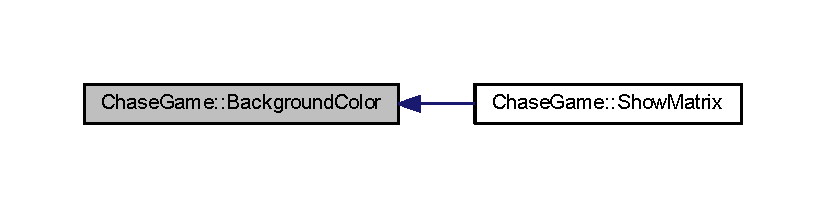
\includegraphics[width=350pt]{namespace_chase_game_ad2dbfd93f4fd5725ab396d5dfa78a0c4_icgraph}
\end{center}
\end{figure}


\hypertarget{namespace_chase_game_a3a7382465f6f23fe77cde4e589fb80d6}{\index{Chase\-Game@{Chase\-Game}!Clear\-Screen@{Clear\-Screen}}
\index{Clear\-Screen@{Clear\-Screen}!ChaseGame@{Chase\-Game}}
\subsubsection[{Clear\-Screen}]{\setlength{\rightskip}{0pt plus 5cm}void Chase\-Game\-::\-Clear\-Screen (
\begin{DoxyParamCaption}
{}
\end{DoxyParamCaption}
)}}\label{namespace_chase_game_a3a7382465f6f23fe77cde4e589fb80d6}


Definition at line 25 of file unix.\-cxx.



Here is the caller graph for this function\-:\nopagebreak
\begin{figure}[H]
\begin{center}
\leavevmode
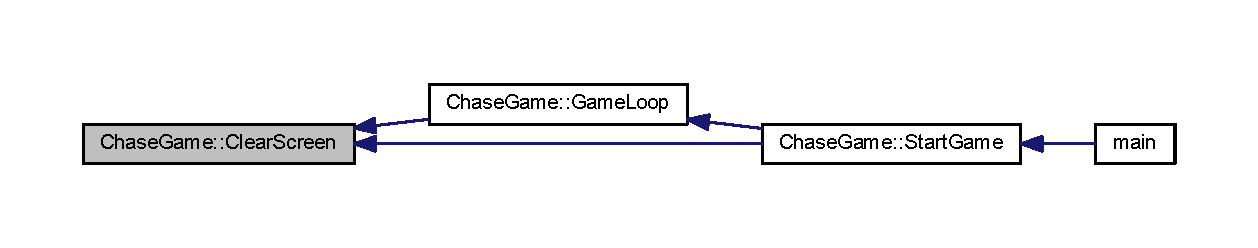
\includegraphics[width=350pt]{namespace_chase_game_a3a7382465f6f23fe77cde4e589fb80d6_icgraph}
\end{center}
\end{figure}


\hypertarget{namespace_chase_game_a3a120300b1e200a26fe8680a33300283}{\index{Chase\-Game@{Chase\-Game}!Color@{Color}}
\index{Color@{Color}!ChaseGame@{Chase\-Game}}
\subsubsection[{Color}]{\setlength{\rightskip}{0pt plus 5cm}void Chase\-Game\-::\-Color (
\begin{DoxyParamCaption}
\item[{const int \&}]{Color}
\end{DoxyParamCaption}
)}}\label{namespace_chase_game_a3a120300b1e200a26fe8680a33300283}


Definition at line 29 of file unix.\-cxx.



Here is the caller graph for this function\-:\nopagebreak
\begin{figure}[H]
\begin{center}
\leavevmode
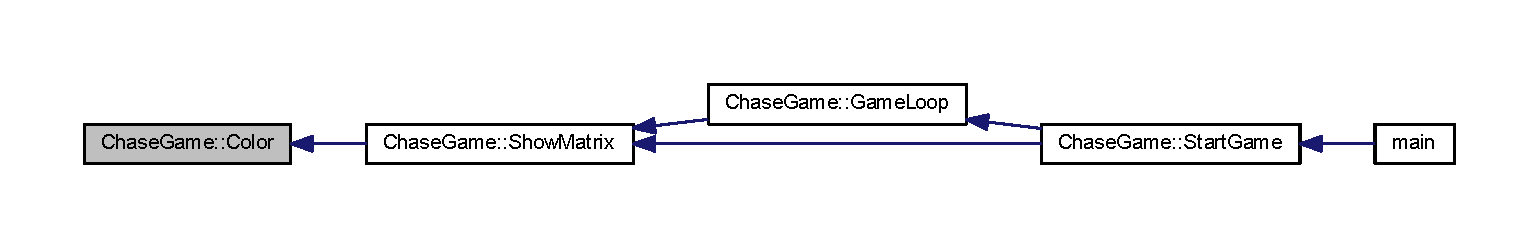
\includegraphics[width=350pt]{namespace_chase_game_a3a120300b1e200a26fe8680a33300283_icgraph}
\end{center}
\end{figure}


\hypertarget{namespace_chase_game_a2bf846fb0618a485e9054b26555ed484}{\index{Chase\-Game@{Chase\-Game}!Game\-Loop@{Game\-Loop}}
\index{Game\-Loop@{Game\-Loop}!ChaseGame@{Chase\-Game}}
\subsubsection[{Game\-Loop}]{\setlength{\rightskip}{0pt plus 5cm}bool Chase\-Game\-::\-Game\-Loop (
\begin{DoxyParamCaption}
\item[{C\-Matrix \&}]{Mat, }
\item[{S\-Map\-Gen\-Params \&}]{Map\-Gen\-Params, }
\item[{S\-Game\-Status \&}]{Config}
\end{DoxyParamCaption}
)}}\label{namespace_chase_game_a2bf846fb0618a485e9054b26555ed484}


This is the game loop. 


\begin{DoxyParams}{Parameters}
{\em Mat} & Game Matrix \\
\hline
{\em Map\-Gen\-Params} & Map generator parameters \\
\hline
{\em Config} & Game configuration \\
\hline
\end{DoxyParams}
\begin{DoxyReturn}{Returns}
true If game is running 

false If game is ended 
\end{DoxyReturn}


Definition at line 41 of file game.\-cxx.



Here is the call graph for this function\-:\nopagebreak
\begin{figure}[H]
\begin{center}
\leavevmode
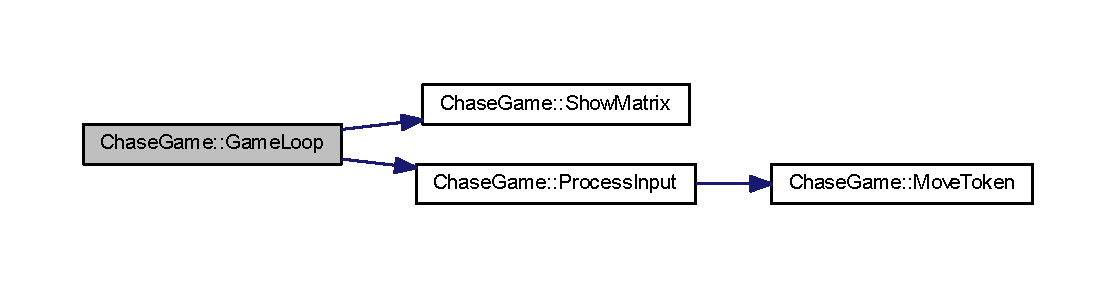
\includegraphics[width=350pt]{namespace_chase_game_a2bf846fb0618a485e9054b26555ed484_cgraph}
\end{center}
\end{figure}




Here is the caller graph for this function\-:\nopagebreak
\begin{figure}[H]
\begin{center}
\leavevmode
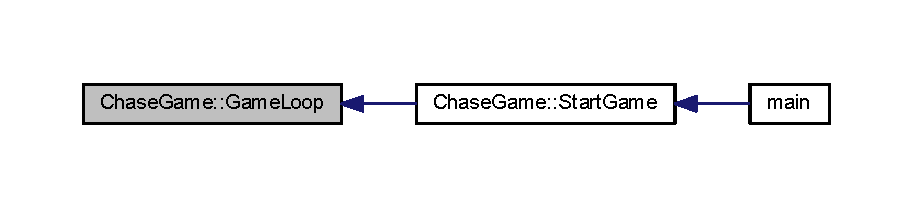
\includegraphics[width=350pt]{namespace_chase_game_a2bf846fb0618a485e9054b26555ed484_icgraph}
\end{center}
\end{figure}


\hypertarget{namespace_chase_game_a15617c8a111cd66bf5d24fd1e82a119d}{\index{Chase\-Game@{Chase\-Game}!Gen\-Map@{Gen\-Map}}
\index{Gen\-Map@{Gen\-Map}!ChaseGame@{Chase\-Game}}
\subsubsection[{Gen\-Map}]{\setlength{\rightskip}{0pt plus 5cm}void Chase\-Game\-::\-Gen\-Map (
\begin{DoxyParamCaption}
\item[{C\-Matrix \&}]{Mat, }
\item[{const S\-Map\-Gen\-Params \&}]{Params, }
\item[{const int}]{Difficulty}
\end{DoxyParamCaption}
)}}\label{namespace_chase_game_a15617c8a111cd66bf5d24fd1e82a119d}


Creates game matrix from the parameters and config file. 


\begin{DoxyParams}{Parameters}
{\em Mat} & Game matrix \\
\hline
{\em Params} & Map parametes \\
\hline
{\em Difficulty} & Game difficulty (higher =$>$ more obstacles) \\
\hline
\end{DoxyParams}


Definition at line 49 of file map.\-cxx.



Here is the call graph for this function\-:
\nopagebreak
\begin{figure}[H]
\begin{center}
\leavevmode
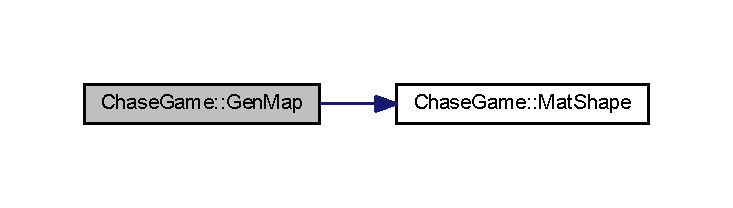
\includegraphics[width=350pt]{namespace_chase_game_a15617c8a111cd66bf5d24fd1e82a119d_cgraph}
\end{center}
\end{figure}




Here is the caller graph for this function\-:
\nopagebreak
\begin{figure}[H]
\begin{center}
\leavevmode
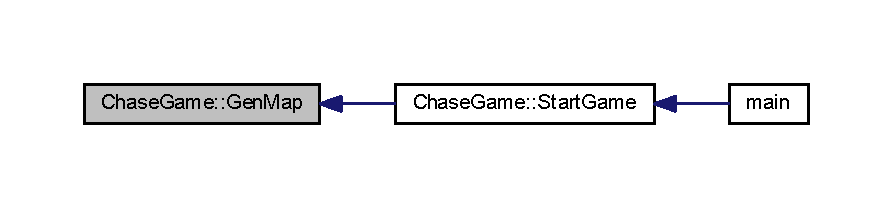
\includegraphics[width=350pt]{namespace_chase_game_a15617c8a111cd66bf5d24fd1e82a119d_icgraph}
\end{center}
\end{figure}


\hypertarget{namespace_chase_game_afa8eec677de5433e0e886da19f7e9c4a}{\index{Chase\-Game@{Chase\-Game}!Get\-Input@{Get\-Input}}
\index{Get\-Input@{Get\-Input}!ChaseGame@{Chase\-Game}}
\subsubsection[{Get\-Input}]{\setlength{\rightskip}{0pt plus 5cm}char Chase\-Game\-::\-Get\-Input (
\begin{DoxyParamCaption}
{}
\end{DoxyParamCaption}
)}}\label{namespace_chase_game_afa8eec677de5433e0e886da19f7e9c4a}


Definition at line 38 of file unix.\-cxx.



Here is the caller graph for this function\-:\nopagebreak
\begin{figure}[H]
\begin{center}
\leavevmode
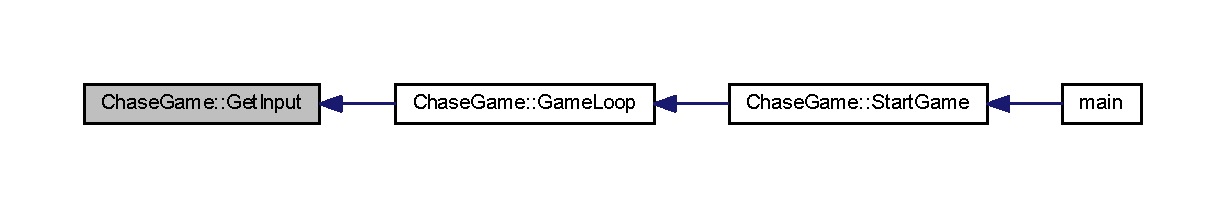
\includegraphics[width=350pt]{namespace_chase_game_afa8eec677de5433e0e886da19f7e9c4a_icgraph}
\end{center}
\end{figure}


\hypertarget{namespace_chase_game_adab063b49bbe754d7cd4992b72da3746}{\index{Chase\-Game@{Chase\-Game}!Init\-Config@{Init\-Config}}
\index{Init\-Config@{Init\-Config}!ChaseGame@{Chase\-Game}}
\subsubsection[{Init\-Config}]{\setlength{\rightskip}{0pt plus 5cm}void Chase\-Game\-::\-Init\-Config (
\begin{DoxyParamCaption}
\item[{S\-Game\-Status \&}]{Config}
\end{DoxyParamCaption}
)}}\label{namespace_chase_game_adab063b49bbe754d7cd4992b72da3746}


This function inits the config. 


\begin{DoxyParams}{Parameters}
{\em Config} & Game config struct \\
\hline
\end{DoxyParams}


Definition at line 59 of file game.\-cxx.

\hypertarget{namespace_chase_game_addd460052ec5a5fe3010665ca84b07ec}{\index{Chase\-Game@{Chase\-Game}!Load\-Game\-Config@{Load\-Game\-Config}}
\index{Load\-Game\-Config@{Load\-Game\-Config}!ChaseGame@{Chase\-Game}}
\subsubsection[{Load\-Game\-Config}]{\setlength{\rightskip}{0pt plus 5cm}{\bf S\-Game\-Status} Chase\-Game\-::\-Load\-Game\-Config (
\begin{DoxyParamCaption}
\item[{const std\-::string \&}]{File\-Name}
\end{DoxyParamCaption}
)}}\label{namespace_chase_game_addd460052ec5a5fe3010665ca84b07ec}


Loads game configuration. 

\begin{DoxyReturn}{Returns}
Game configuration structure loaded from file or default config 
\end{DoxyReturn}


Definition at line 87 of file file.\-cxx.



Here is the call graph for this function\-:\nopagebreak
\begin{figure}[H]
\begin{center}
\leavevmode
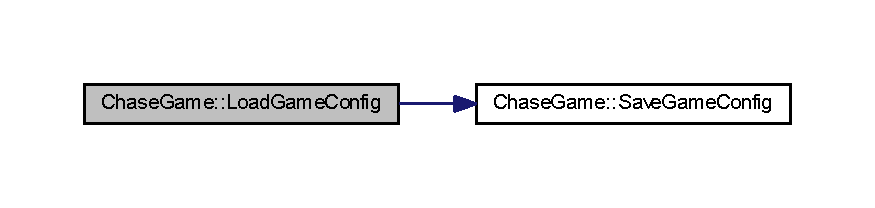
\includegraphics[width=350pt]{namespace_chase_game_addd460052ec5a5fe3010665ca84b07ec_cgraph}
\end{center}
\end{figure}




Here is the caller graph for this function\-:\nopagebreak
\begin{figure}[H]
\begin{center}
\leavevmode
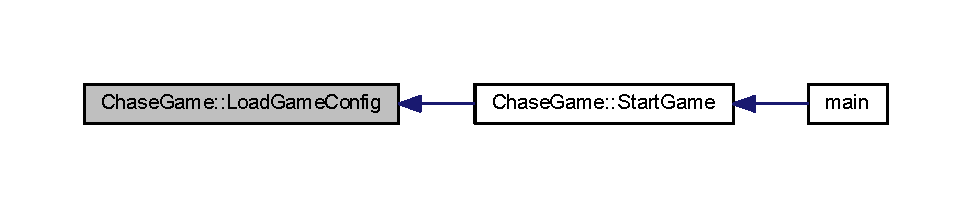
\includegraphics[width=350pt]{namespace_chase_game_addd460052ec5a5fe3010665ca84b07ec_icgraph}
\end{center}
\end{figure}


\hypertarget{namespace_chase_game_a9c5b5d91cb4251cae461faa4ace8a0cf}{\index{Chase\-Game@{Chase\-Game}!Load\-Map\-Gen\-Config@{Load\-Map\-Gen\-Config}}
\index{Load\-Map\-Gen\-Config@{Load\-Map\-Gen\-Config}!ChaseGame@{Chase\-Game}}
\subsubsection[{Load\-Map\-Gen\-Config}]{\setlength{\rightskip}{0pt plus 5cm}{\bf S\-Map\-Gen\-Params} Chase\-Game\-::\-Load\-Map\-Gen\-Config (
\begin{DoxyParamCaption}
\item[{const std\-::string \&}]{File\-Name}
\end{DoxyParamCaption}
)}}\label{namespace_chase_game_a9c5b5d91cb4251cae461faa4ace8a0cf}


Loads parameters from a config file. 


\begin{DoxyParams}{Parameters}
{\em File\-Name} & Config filename \\
\hline
\end{DoxyParams}
\begin{DoxyReturn}{Returns}
Map generator parametors loaded from file or default config 
\end{DoxyReturn}
\hypertarget{namespace_chase_game_a4779af792d3de8e274049bf2019e0343}{\index{Chase\-Game@{Chase\-Game}!Load\-Map\-Gen\-Config@{Load\-Map\-Gen\-Config}}
\index{Load\-Map\-Gen\-Config@{Load\-Map\-Gen\-Config}!ChaseGame@{Chase\-Game}}
\subsubsection[{Load\-Map\-Gen\-Config}]{\setlength{\rightskip}{0pt plus 5cm}{\bf S\-Map\-Gen\-Params} Chase\-Game\-::\-Load\-Map\-Gen\-Config (
\begin{DoxyParamCaption}
\item[{const string \&}]{File\-Name}
\end{DoxyParamCaption}
)}}\label{namespace_chase_game_a4779af792d3de8e274049bf2019e0343}


Definition at line 24 of file file.\-cxx.



Here is the call graph for this function\-:\nopagebreak
\begin{figure}[H]
\begin{center}
\leavevmode
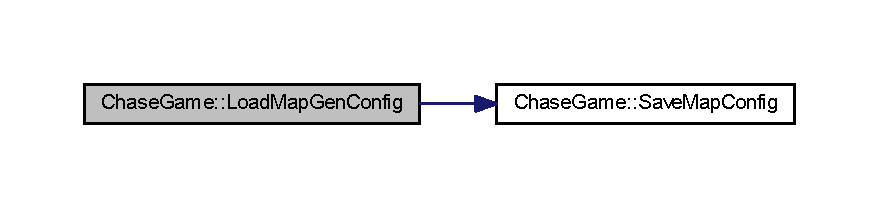
\includegraphics[width=350pt]{namespace_chase_game_a4779af792d3de8e274049bf2019e0343_cgraph}
\end{center}
\end{figure}




Here is the caller graph for this function\-:\nopagebreak
\begin{figure}[H]
\begin{center}
\leavevmode
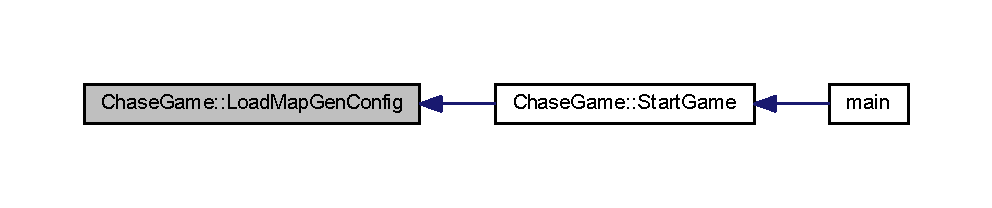
\includegraphics[width=350pt]{namespace_chase_game_a4779af792d3de8e274049bf2019e0343_icgraph}
\end{center}
\end{figure}


\hypertarget{namespace_chase_game_a049d8d8beb22431889ca7ba34cc90871}{\index{Chase\-Game@{Chase\-Game}!Mat\-Shape@{Mat\-Shape}}
\index{Mat\-Shape@{Mat\-Shape}!ChaseGame@{Chase\-Game}}
\subsubsection[{Mat\-Shape}]{\setlength{\rightskip}{0pt plus 5cm}void Chase\-Game\-::\-Mat\-Shape (
\begin{DoxyParamCaption}
\item[{C\-Matrix \&}]{Mat, }
\item[{const std\-::array$<$ bool, 9 $>$}]{Tab, }
\item[{const unsigned}]{Y, }
\item[{const unsigned}]{X}
\end{DoxyParamCaption}
)}}\label{namespace_chase_game_a049d8d8beb22431889ca7ba34cc90871}


Generate a random shape in the map. 


\begin{DoxyParams}{Parameters}
{\em Mat} & Game matrix \\
\hline
{\em Tab} & Shape \\
\hline
{\em Y} & The y position \\
\hline
{\em X} & The x position \\
\hline
\end{DoxyParams}
\hypertarget{namespace_chase_game_ac12626138d0e2c49669eba73ffb4e4b7}{\index{Chase\-Game@{Chase\-Game}!Mat\-Shape@{Mat\-Shape}}
\index{Mat\-Shape@{Mat\-Shape}!ChaseGame@{Chase\-Game}}
\subsubsection[{Mat\-Shape}]{\setlength{\rightskip}{0pt plus 5cm}void Chase\-Game\-::\-Mat\-Shape (
\begin{DoxyParamCaption}
\item[{C\-Matrix \&}]{Mat, }
\item[{const array$<$ bool, 9 $>$}]{Tab, }
\item[{const unsigned}]{Y, }
\item[{const unsigned}]{X}
\end{DoxyParamCaption}
)}}\label{namespace_chase_game_ac12626138d0e2c49669eba73ffb4e4b7}


Definition at line 27 of file map.\-cxx.



Here is the caller graph for this function\-:
\nopagebreak
\begin{figure}[H]
\begin{center}
\leavevmode
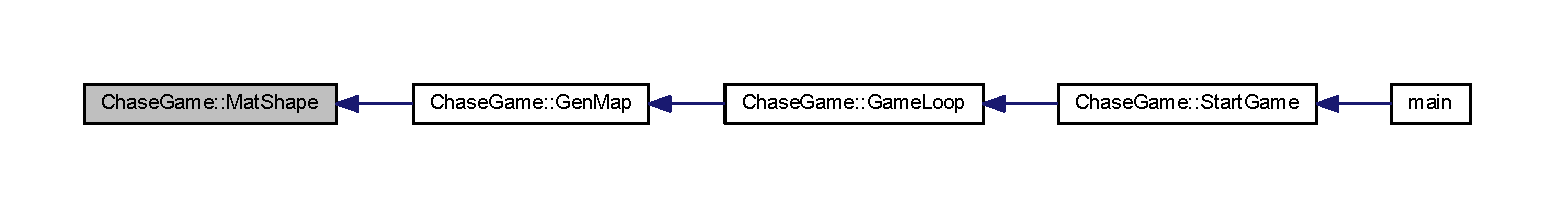
\includegraphics[width=350pt]{namespace_chase_game_ac12626138d0e2c49669eba73ffb4e4b7_icgraph}
\end{center}
\end{figure}


\hypertarget{namespace_chase_game_a1dfe4bdbd50ee18cf85760219ea90b03}{\index{Chase\-Game@{Chase\-Game}!Move\-Token@{Move\-Token}}
\index{Move\-Token@{Move\-Token}!ChaseGame@{Chase\-Game}}
\subsubsection[{Move\-Token}]{\setlength{\rightskip}{0pt plus 5cm}char Chase\-Game\-::\-Move\-Token (
\begin{DoxyParamCaption}
\item[{C\-Matrix \&}]{Mat, }
\item[{const char}]{Move, }
\item[{S\-Player\-Pos \&}]{Pos, }
\item[{const S\-Player\-Keys \&}]{Key\-Codes}
\end{DoxyParamCaption}
)}}\label{namespace_chase_game_a1dfe4bdbd50ee18cf85760219ea90b03}


Move a token in the game matrix. 


\begin{DoxyParams}{Parameters}
{\em Mat} & Game matrix \\
\hline
{\em Move} & Move code \\
\hline
{\em Pos} & Token position \\
\hline
{\em Key\-Codes} & Player specific key codes for movement \\
\hline
\end{DoxyParams}
\begin{DoxyReturn}{Returns}
Replaced char 
\end{DoxyReturn}


Definition at line 146 of file map.\-cxx.



Here is the caller graph for this function\-:\nopagebreak
\begin{figure}[H]
\begin{center}
\leavevmode
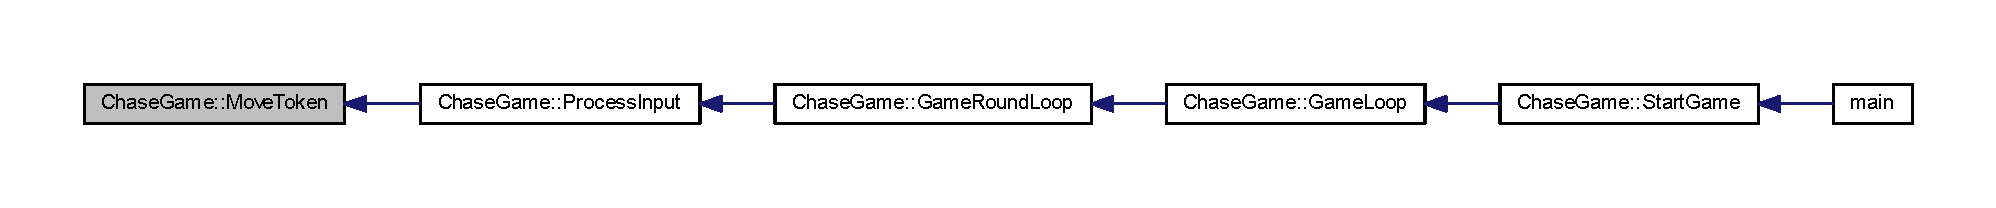
\includegraphics[width=350pt]{namespace_chase_game_a1dfe4bdbd50ee18cf85760219ea90b03_icgraph}
\end{center}
\end{figure}


\hypertarget{namespace_chase_game_ab5112517855da810fe3b7bdb81d58484}{\index{Chase\-Game@{Chase\-Game}!Process\-Input@{Process\-Input}}
\index{Process\-Input@{Process\-Input}!ChaseGame@{Chase\-Game}}
\subsubsection[{Process\-Input}]{\setlength{\rightskip}{0pt plus 5cm}char Chase\-Game\-::\-Process\-Input (
\begin{DoxyParamCaption}
\item[{C\-Matrix \&}]{Mat, }
\item[{const char}]{Input, }
\item[{S\-Game\-Status \&}]{Config}
\end{DoxyParamCaption}
)}}\label{namespace_chase_game_ab5112517855da810fe3b7bdb81d58484}


Processes user input. 


\begin{DoxyParams}{Parameters}
{\em Mat} & Game Matrix \\
\hline
{\em Input} & input given \\
\hline
{\em Config} & Game configuration \\
\hline
\end{DoxyParams}
\begin{DoxyReturn}{Returns}
Chararcter representing the replaced charachter while moving 

K\-Cancelled if the move was cancelled 
\end{DoxyReturn}


Definition at line 28 of file game.\-cxx.



Here is the call graph for this function\-:\nopagebreak
\begin{figure}[H]
\begin{center}
\leavevmode
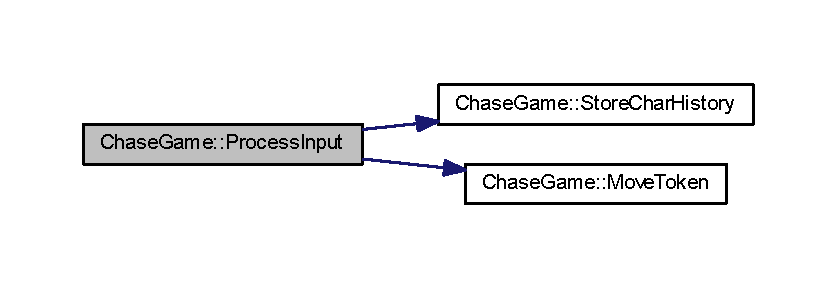
\includegraphics[width=350pt]{namespace_chase_game_ab5112517855da810fe3b7bdb81d58484_cgraph}
\end{center}
\end{figure}




Here is the caller graph for this function\-:\nopagebreak
\begin{figure}[H]
\begin{center}
\leavevmode
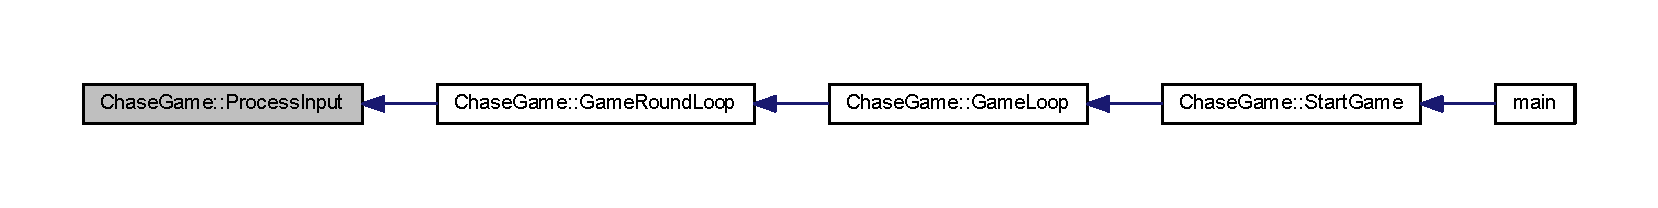
\includegraphics[width=350pt]{namespace_chase_game_ab5112517855da810fe3b7bdb81d58484_icgraph}
\end{center}
\end{figure}


\hypertarget{namespace_chase_game_a561c85a018e34c8baa21f7f500a3c9c7}{\index{Chase\-Game@{Chase\-Game}!Save\-Game\-Config@{Save\-Game\-Config}}
\index{Save\-Game\-Config@{Save\-Game\-Config}!ChaseGame@{Chase\-Game}}
\subsubsection[{Save\-Game\-Config}]{\setlength{\rightskip}{0pt plus 5cm}bool Chase\-Game\-::\-Save\-Game\-Config (
\begin{DoxyParamCaption}
\item[{const std\-::string \&}]{File\-Name, }
\item[{S\-Game\-Status \&}]{Config}
\end{DoxyParamCaption}
)}}\label{namespace_chase_game_a561c85a018e34c8baa21f7f500a3c9c7}


Saves game configuration in a config file. 


\begin{DoxyParams}{Parameters}
{\em File\-Name} & Config filename \\
\hline
{\em Config} & Config to write in the file \\
\hline
\end{DoxyParams}
\begin{DoxyReturn}{Returns}
true if write was successfull 

false if write error 
\end{DoxyReturn}
\hypertarget{namespace_chase_game_a39f8b039151b1a3eef82fdc1c6f52091}{\index{Chase\-Game@{Chase\-Game}!Save\-Game\-Config@{Save\-Game\-Config}}
\index{Save\-Game\-Config@{Save\-Game\-Config}!ChaseGame@{Chase\-Game}}
\subsubsection[{Save\-Game\-Config}]{\setlength{\rightskip}{0pt plus 5cm}bool Chase\-Game\-::\-Save\-Game\-Config (
\begin{DoxyParamCaption}
\item[{const string \&}]{File\-Name, }
\item[{S\-Game\-Status \&}]{Config}
\end{DoxyParamCaption}
)}}\label{namespace_chase_game_a39f8b039151b1a3eef82fdc1c6f52091}


Definition at line 168 of file file.\-cxx.



Here is the caller graph for this function\-:\nopagebreak
\begin{figure}[H]
\begin{center}
\leavevmode
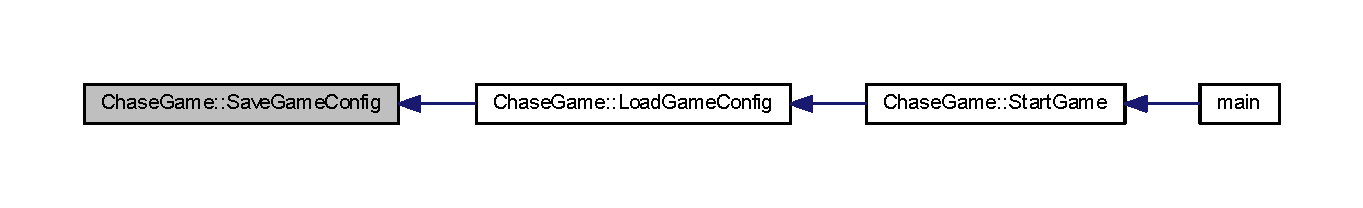
\includegraphics[width=350pt]{namespace_chase_game_a39f8b039151b1a3eef82fdc1c6f52091_icgraph}
\end{center}
\end{figure}


\hypertarget{namespace_chase_game_a4c62f61c6aac5bf06292aa51294fd211}{\index{Chase\-Game@{Chase\-Game}!Save\-Map\-Config@{Save\-Map\-Config}}
\index{Save\-Map\-Config@{Save\-Map\-Config}!ChaseGame@{Chase\-Game}}
\subsubsection[{Save\-Map\-Config}]{\setlength{\rightskip}{0pt plus 5cm}bool Chase\-Game\-::\-Save\-Map\-Config (
\begin{DoxyParamCaption}
\item[{const std\-::string \&}]{File\-Name, }
\item[{S\-Map\-Gen\-Params \&}]{Params}
\end{DoxyParamCaption}
)}}\label{namespace_chase_game_a4c62f61c6aac5bf06292aa51294fd211}


Saves parameters in a config file. 


\begin{DoxyParams}{Parameters}
{\em File\-Name} & Config filename \\
\hline
{\em Params} & Map config to write in the file \\
\hline
\end{DoxyParams}
\begin{DoxyReturn}{Returns}
true if write was successfull, 

false if write error 
\end{DoxyReturn}
\hypertarget{namespace_chase_game_a98e8d90127c802c1445266e39966c3fb}{\index{Chase\-Game@{Chase\-Game}!Save\-Map\-Config@{Save\-Map\-Config}}
\index{Save\-Map\-Config@{Save\-Map\-Config}!ChaseGame@{Chase\-Game}}
\subsubsection[{Save\-Map\-Config}]{\setlength{\rightskip}{0pt plus 5cm}bool Chase\-Game\-::\-Save\-Map\-Config (
\begin{DoxyParamCaption}
\item[{const string \&}]{File\-Name, }
\item[{S\-Map\-Gen\-Params \&}]{Params}
\end{DoxyParamCaption}
)}}\label{namespace_chase_game_a98e8d90127c802c1445266e39966c3fb}


Definition at line 70 of file file.\-cxx.



Here is the caller graph for this function\-:\nopagebreak
\begin{figure}[H]
\begin{center}
\leavevmode
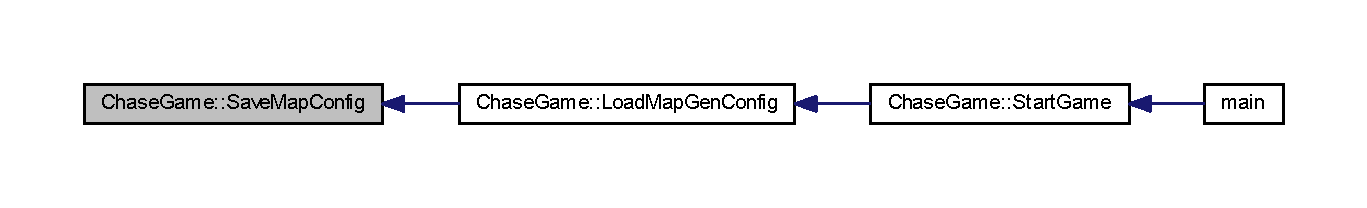
\includegraphics[width=350pt]{namespace_chase_game_a98e8d90127c802c1445266e39966c3fb_icgraph}
\end{center}
\end{figure}


\hypertarget{namespace_chase_game_a871395f1f12e55eaa3d341b8ef2cbb78}{\index{Chase\-Game@{Chase\-Game}!Show\-Matrix@{Show\-Matrix}}
\index{Show\-Matrix@{Show\-Matrix}!ChaseGame@{Chase\-Game}}
\subsubsection[{Show\-Matrix}]{\setlength{\rightskip}{0pt plus 5cm}void Chase\-Game\-::\-Show\-Matrix (
\begin{DoxyParamCaption}
\item[{const C\-Matrix \&}]{Mat, }
\item[{const S\-Color\-Set \&}]{Color\-Set}
\end{DoxyParamCaption}
)}}\label{namespace_chase_game_a871395f1f12e55eaa3d341b8ef2cbb78}


Displays game matrix. 


\begin{DoxyParams}{Parameters}
{\em Mat} & Game matrix \\
\hline
{\em Color\-Set} & Colors to use \\
\hline
\end{DoxyParams}


Definition at line 175 of file map.\-cxx.



Here is the call graph for this function\-:\nopagebreak
\begin{figure}[H]
\begin{center}
\leavevmode
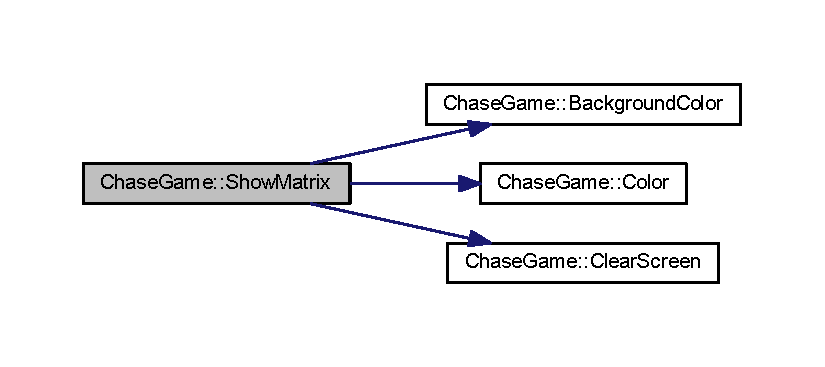
\includegraphics[width=350pt]{namespace_chase_game_a871395f1f12e55eaa3d341b8ef2cbb78_cgraph}
\end{center}
\end{figure}




Here is the caller graph for this function\-:\nopagebreak
\begin{figure}[H]
\begin{center}
\leavevmode
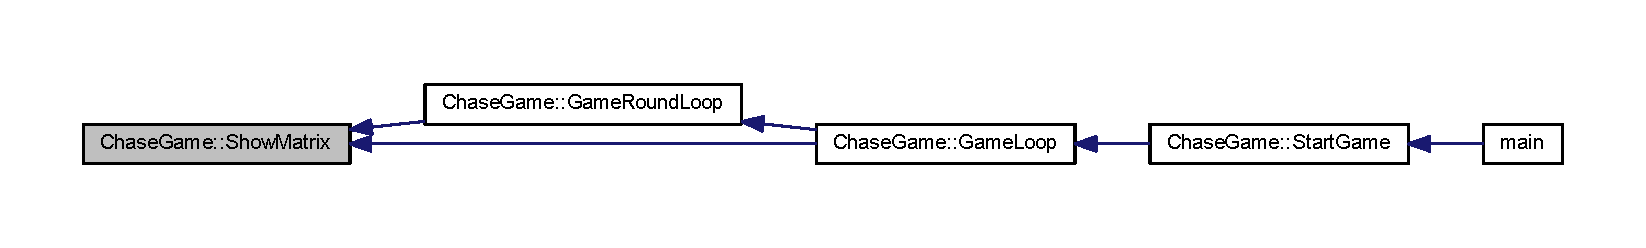
\includegraphics[width=350pt]{namespace_chase_game_a871395f1f12e55eaa3d341b8ef2cbb78_icgraph}
\end{center}
\end{figure}


\hypertarget{namespace_chase_game_a528073d13296b3cf84a6ae07c3550e74}{\index{Chase\-Game@{Chase\-Game}!Start\-Game@{Start\-Game}}
\index{Start\-Game@{Start\-Game}!ChaseGame@{Chase\-Game}}
\subsubsection[{Start\-Game}]{\setlength{\rightskip}{0pt plus 5cm}void Chase\-Game\-::\-Start\-Game (
\begin{DoxyParamCaption}
{}
\end{DoxyParamCaption}
)}}\label{namespace_chase_game_a528073d13296b3cf84a6ae07c3550e74}


This function starts the game. 



Definition at line 74 of file game.\-cxx.



Here is the call graph for this function\-:
\nopagebreak
\begin{figure}[H]
\begin{center}
\leavevmode
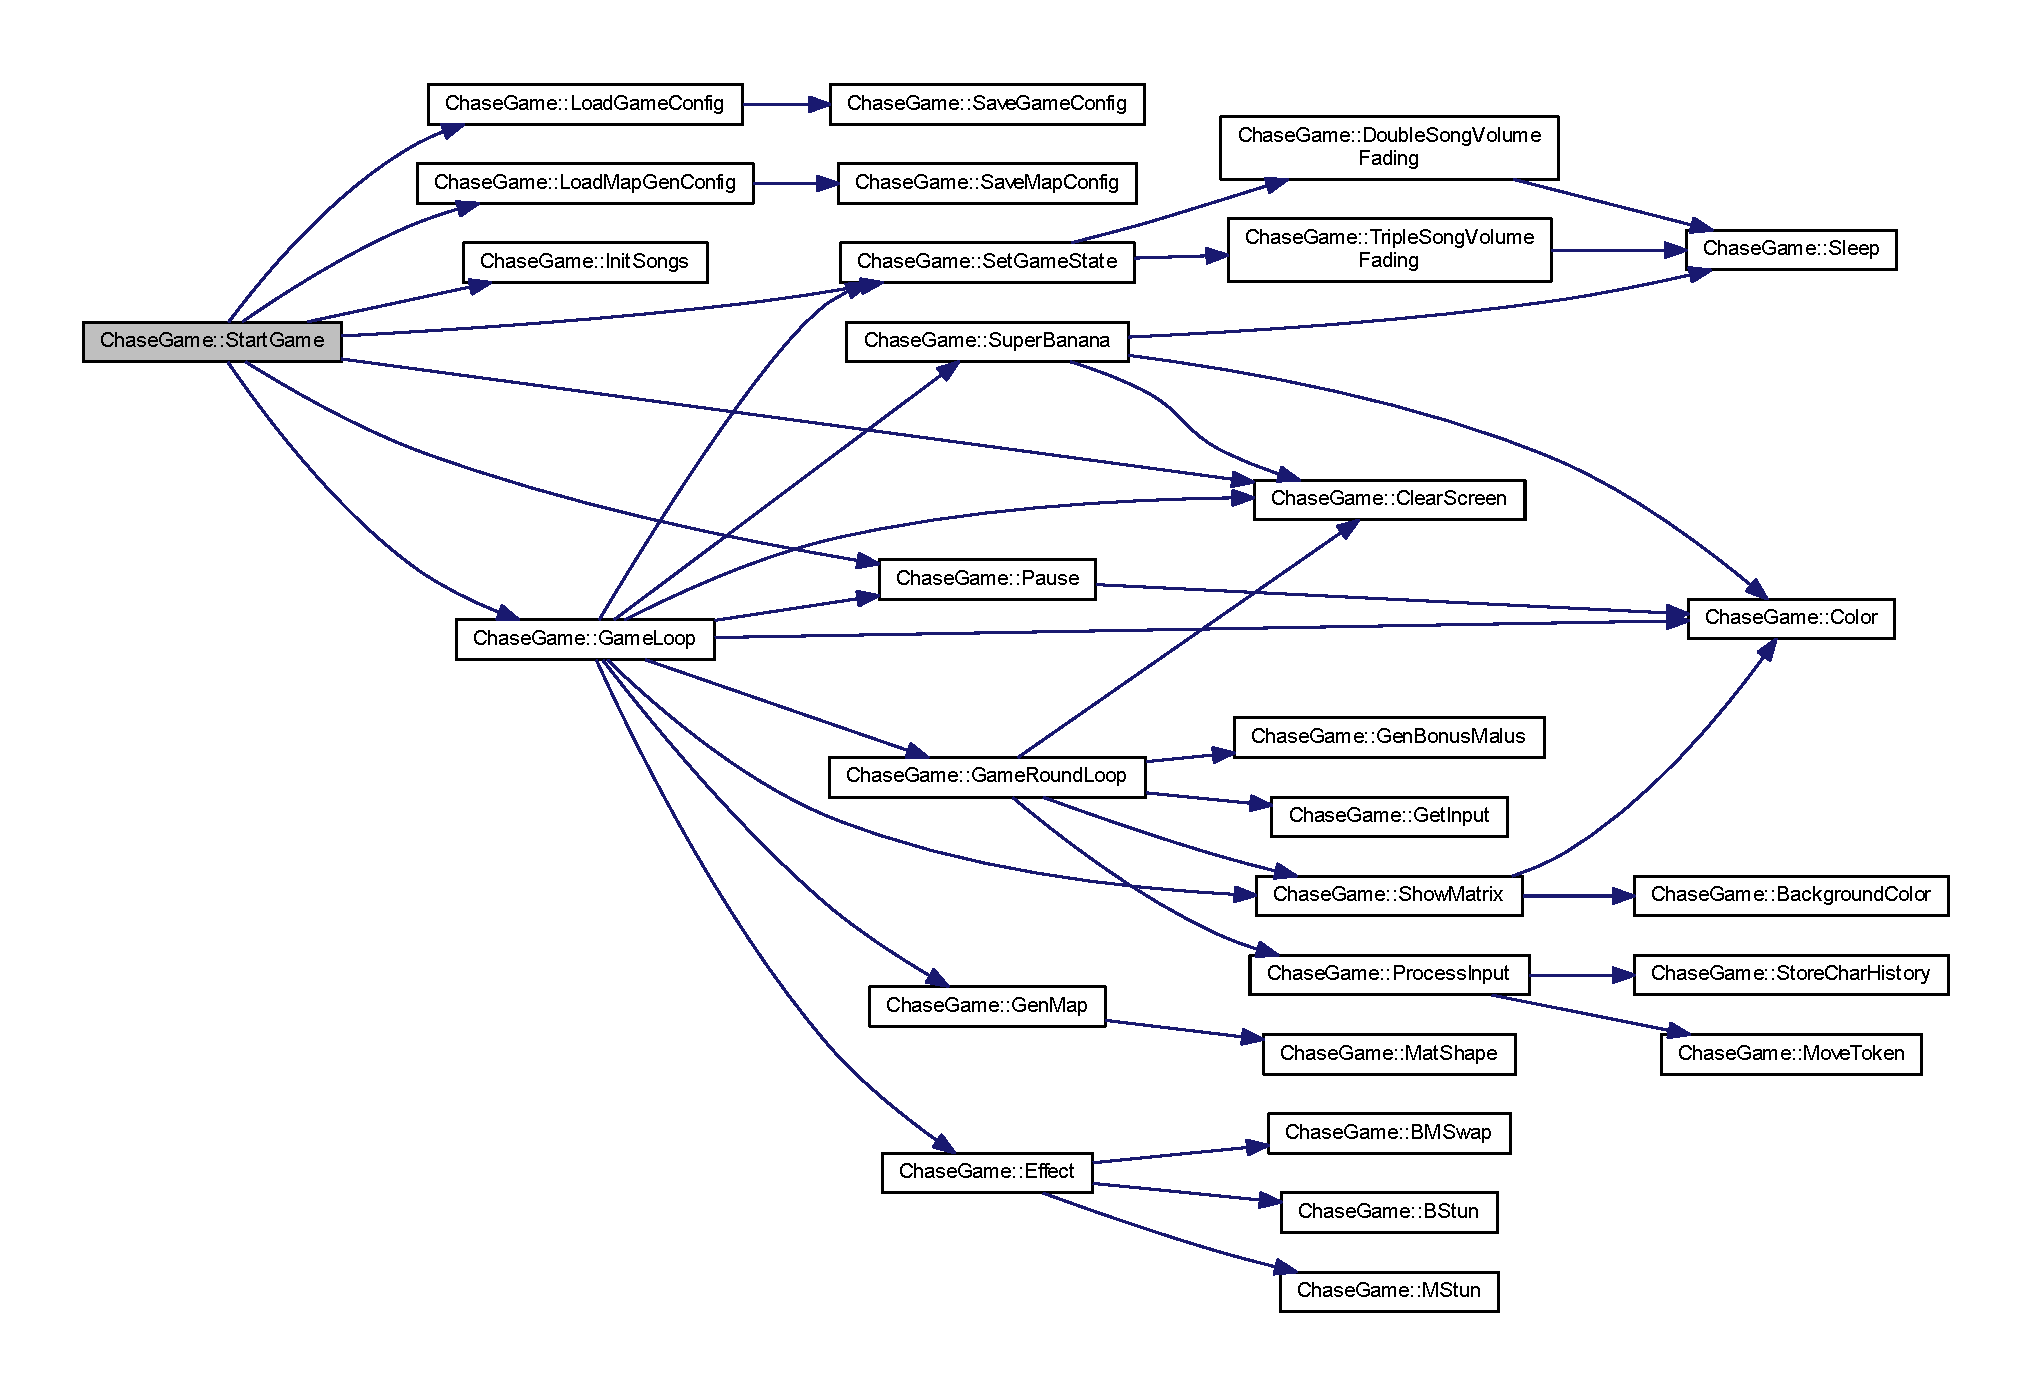
\includegraphics[width=350pt]{namespace_chase_game_a528073d13296b3cf84a6ae07c3550e74_cgraph}
\end{center}
\end{figure}




Here is the caller graph for this function\-:\nopagebreak
\begin{figure}[H]
\begin{center}
\leavevmode
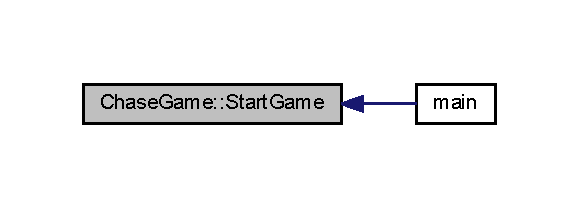
\includegraphics[width=278pt]{namespace_chase_game_a528073d13296b3cf84a6ae07c3550e74_icgraph}
\end{center}
\end{figure}




\subsection{Variable Documentation}
\hypertarget{namespace_chase_game_a12d6411bb9a72150acba6060bb1587e1}{\index{Chase\-Game@{Chase\-Game}!K\-Cancelled@{K\-Cancelled}}
\index{K\-Cancelled@{K\-Cancelled}!ChaseGame@{Chase\-Game}}
\subsubsection[{K\-Cancelled}]{\setlength{\rightskip}{0pt plus 5cm}const char Chase\-Game\-::\-K\-Cancelled = '0'}}\label{namespace_chase_game_a12d6411bb9a72150acba6060bb1587e1}


Character sent when a move is not allowed. 



Definition at line 53 of file globals.\-hxx.

\hypertarget{namespace_chase_game_aa036d4de40188ba2e1aa36ab6cfaf1da}{\index{Chase\-Game@{Chase\-Game}!K\-Empty@{K\-Empty}}
\index{K\-Empty@{K\-Empty}!ChaseGame@{Chase\-Game}}
\subsubsection[{K\-Empty}]{\setlength{\rightskip}{0pt plus 5cm}const char Chase\-Game\-::\-K\-Empty = ' '}}\label{namespace_chase_game_aa036d4de40188ba2e1aa36ab6cfaf1da}


Character representing voidness. 



Definition at line 47 of file globals.\-hxx.

\hypertarget{namespace_chase_game_ad86181b2050b912dab9d69d2f0bea76e}{\index{Chase\-Game@{Chase\-Game}!K\-Obstacle@{K\-Obstacle}}
\index{K\-Obstacle@{K\-Obstacle}!ChaseGame@{Chase\-Game}}
\subsubsection[{K\-Obstacle}]{\setlength{\rightskip}{0pt plus 5cm}const char Chase\-Game\-::\-K\-Obstacle = '\#'}}\label{namespace_chase_game_ad86181b2050b912dab9d69d2f0bea76e}


Character representing obstacles and walls. 



Definition at line 50 of file globals.\-hxx.

\hypertarget{namespace_chase_game_a8452e2d6de618e4ca7a9f76b082b52a4}{\index{Chase\-Game@{Chase\-Game}!K\-Token\-Player1@{K\-Token\-Player1}}
\index{K\-Token\-Player1@{K\-Token\-Player1}!ChaseGame@{Chase\-Game}}
\subsubsection[{K\-Token\-Player1}]{\setlength{\rightskip}{0pt plus 5cm}const char Chase\-Game\-::\-K\-Token\-Player1 = 'X'}}\label{namespace_chase_game_a8452e2d6de618e4ca7a9f76b082b52a4}


Character representing player one. 



Definition at line 41 of file globals.\-hxx.

\hypertarget{namespace_chase_game_ae27343407c21a8d6e3cf26b736bd5527}{\index{Chase\-Game@{Chase\-Game}!K\-Token\-Player2@{K\-Token\-Player2}}
\index{K\-Token\-Player2@{K\-Token\-Player2}!ChaseGame@{Chase\-Game}}
\subsubsection[{K\-Token\-Player2}]{\setlength{\rightskip}{0pt plus 5cm}const char Chase\-Game\-::\-K\-Token\-Player2 = 'O'}}\label{namespace_chase_game_ae27343407c21a8d6e3cf26b736bd5527}


Character representing player two. 



Definition at line 44 of file globals.\-hxx.


\chapter{Class Documentation}
\hypertarget{struct_chase_game_1_1_s_color_set}{\section{Chase\-Game\-:\-:S\-Color\-Set Struct Reference}
\label{struct_chase_game_1_1_s_color_set}\index{Chase\-Game\-::\-S\-Color\-Set@{Chase\-Game\-::\-S\-Color\-Set}}
}


Color set to use when displaying the map.  




{\ttfamily \#include $<$globals.\-hxx$>$}

\subsection*{Public Attributes}
\begin{DoxyCompactItemize}
\item 
int \hyperlink{struct_chase_game_1_1_s_color_set_a51e5a557359624fe92be93cb80621922}{Color\-P1}
\begin{DoxyCompactList}\small\item\em Color value representing player one. \end{DoxyCompactList}\item 
int \hyperlink{struct_chase_game_1_1_s_color_set_a777bce7519236b269ba44d921f54e4e8}{Color\-P2}
\begin{DoxyCompactList}\small\item\em Color value representing player two. \end{DoxyCompactList}\item 
int \hyperlink{struct_chase_game_1_1_s_color_set_acb1e4df5c042ae8ca8a66d7de26a9148}{Color\-Obstacle}
\begin{DoxyCompactList}\small\item\em Color value representing an obstacle. \end{DoxyCompactList}\item 
int \hyperlink{struct_chase_game_1_1_s_color_set_a7a7a8dae118390ce5b4432aa4d99a474}{Color\-Wall}
\begin{DoxyCompactList}\small\item\em Color value representing a wall. \end{DoxyCompactList}\item 
int \hyperlink{struct_chase_game_1_1_s_color_set_aacd34496b36640358ecae127f6bb6cc4}{Color\-Bonus}
\begin{DoxyCompactList}\small\item\em Color value representing a bonus. \end{DoxyCompactList}\item 
int \hyperlink{struct_chase_game_1_1_s_color_set_aa2eb52b7d1fb4059da9935a230715498}{Color\-Malus}
\begin{DoxyCompactList}\small\item\em Color value representing a malus. \end{DoxyCompactList}\end{DoxyCompactItemize}


\subsection{Detailed Description}
Color set to use when displaying the map. 

Definition at line 112 of file globals.\-hxx.



\subsection{Member Data Documentation}
\hypertarget{struct_chase_game_1_1_s_color_set_aacd34496b36640358ecae127f6bb6cc4}{\index{Chase\-Game\-::\-S\-Color\-Set@{Chase\-Game\-::\-S\-Color\-Set}!Color\-Bonus@{Color\-Bonus}}
\index{Color\-Bonus@{Color\-Bonus}!ChaseGame::SColorSet@{Chase\-Game\-::\-S\-Color\-Set}}
\subsubsection[{Color\-Bonus}]{\setlength{\rightskip}{0pt plus 5cm}int Chase\-Game\-::\-S\-Color\-Set\-::\-Color\-Bonus}}\label{struct_chase_game_1_1_s_color_set_aacd34496b36640358ecae127f6bb6cc4}


Color value representing a bonus. 



Definition at line 122 of file globals.\-hxx.

\hypertarget{struct_chase_game_1_1_s_color_set_aa2eb52b7d1fb4059da9935a230715498}{\index{Chase\-Game\-::\-S\-Color\-Set@{Chase\-Game\-::\-S\-Color\-Set}!Color\-Malus@{Color\-Malus}}
\index{Color\-Malus@{Color\-Malus}!ChaseGame::SColorSet@{Chase\-Game\-::\-S\-Color\-Set}}
\subsubsection[{Color\-Malus}]{\setlength{\rightskip}{0pt plus 5cm}int Chase\-Game\-::\-S\-Color\-Set\-::\-Color\-Malus}}\label{struct_chase_game_1_1_s_color_set_aa2eb52b7d1fb4059da9935a230715498}


Color value representing a malus. 



Definition at line 124 of file globals.\-hxx.

\hypertarget{struct_chase_game_1_1_s_color_set_acb1e4df5c042ae8ca8a66d7de26a9148}{\index{Chase\-Game\-::\-S\-Color\-Set@{Chase\-Game\-::\-S\-Color\-Set}!Color\-Obstacle@{Color\-Obstacle}}
\index{Color\-Obstacle@{Color\-Obstacle}!ChaseGame::SColorSet@{Chase\-Game\-::\-S\-Color\-Set}}
\subsubsection[{Color\-Obstacle}]{\setlength{\rightskip}{0pt plus 5cm}int Chase\-Game\-::\-S\-Color\-Set\-::\-Color\-Obstacle}}\label{struct_chase_game_1_1_s_color_set_acb1e4df5c042ae8ca8a66d7de26a9148}


Color value representing an obstacle. 



Definition at line 118 of file globals.\-hxx.

\hypertarget{struct_chase_game_1_1_s_color_set_a51e5a557359624fe92be93cb80621922}{\index{Chase\-Game\-::\-S\-Color\-Set@{Chase\-Game\-::\-S\-Color\-Set}!Color\-P1@{Color\-P1}}
\index{Color\-P1@{Color\-P1}!ChaseGame::SColorSet@{Chase\-Game\-::\-S\-Color\-Set}}
\subsubsection[{Color\-P1}]{\setlength{\rightskip}{0pt plus 5cm}int Chase\-Game\-::\-S\-Color\-Set\-::\-Color\-P1}}\label{struct_chase_game_1_1_s_color_set_a51e5a557359624fe92be93cb80621922}


Color value representing player one. 



Definition at line 114 of file globals.\-hxx.

\hypertarget{struct_chase_game_1_1_s_color_set_a777bce7519236b269ba44d921f54e4e8}{\index{Chase\-Game\-::\-S\-Color\-Set@{Chase\-Game\-::\-S\-Color\-Set}!Color\-P2@{Color\-P2}}
\index{Color\-P2@{Color\-P2}!ChaseGame::SColorSet@{Chase\-Game\-::\-S\-Color\-Set}}
\subsubsection[{Color\-P2}]{\setlength{\rightskip}{0pt plus 5cm}int Chase\-Game\-::\-S\-Color\-Set\-::\-Color\-P2}}\label{struct_chase_game_1_1_s_color_set_a777bce7519236b269ba44d921f54e4e8}


Color value representing player two. 



Definition at line 116 of file globals.\-hxx.

\hypertarget{struct_chase_game_1_1_s_color_set_a7a7a8dae118390ce5b4432aa4d99a474}{\index{Chase\-Game\-::\-S\-Color\-Set@{Chase\-Game\-::\-S\-Color\-Set}!Color\-Wall@{Color\-Wall}}
\index{Color\-Wall@{Color\-Wall}!ChaseGame::SColorSet@{Chase\-Game\-::\-S\-Color\-Set}}
\subsubsection[{Color\-Wall}]{\setlength{\rightskip}{0pt plus 5cm}int Chase\-Game\-::\-S\-Color\-Set\-::\-Color\-Wall}}\label{struct_chase_game_1_1_s_color_set_a7a7a8dae118390ce5b4432aa4d99a474}


Color value representing a wall. 



Definition at line 120 of file globals.\-hxx.



The documentation for this struct was generated from the following file\-:\begin{DoxyCompactItemize}
\item 
C\-:/\-Development/\-I\-U\-T/git -\/ Copie/projet/\hyperlink{globals_8hxx}{globals.\-hxx}\end{DoxyCompactItemize}

\hypertarget{struct_chase_game_1_1_s_game_status}{\section{Chase\-Game\-:\-:S\-Game\-Status Struct Reference}
\label{struct_chase_game_1_1_s_game_status}\index{Chase\-Game\-::\-S\-Game\-Status@{Chase\-Game\-::\-S\-Game\-Status}}
}


Contains game configuration.  




{\ttfamily \#include $<$globals.\-hxx$>$}



Collaboration diagram for Chase\-Game\-:\-:S\-Game\-Status\-:\nopagebreak
\begin{figure}[H]
\begin{center}
\leavevmode
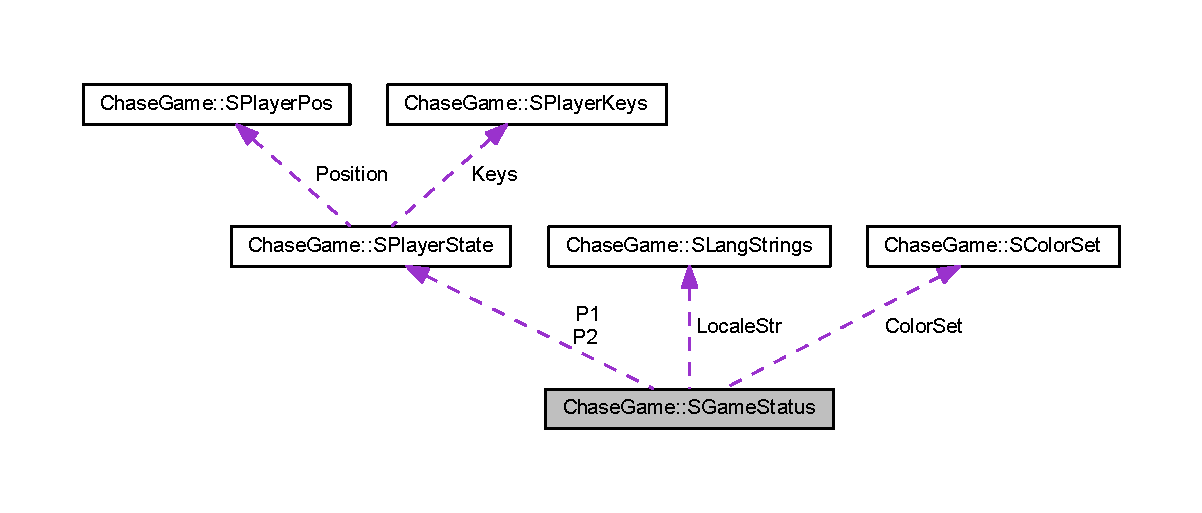
\includegraphics[width=350pt]{struct_chase_game_1_1_s_game_status__coll__graph}
\end{center}
\end{figure}
\subsection*{Public Attributes}
\begin{DoxyCompactItemize}
\item 
char \hyperlink{struct_chase_game_1_1_s_game_status_aaa0cca00432a2ac7fae4be521164f5c2}{Key\-Pause}
\begin{DoxyCompactList}\small\item\em Key to pause the game. \end{DoxyCompactList}\item 
char \hyperlink{struct_chase_game_1_1_s_game_status_a6a88e0903d13f10f4fcf8050157b2bdb}{Key\-Exit}
\begin{DoxyCompactList}\small\item\em Key to exit the game. \end{DoxyCompactList}\item 
\hyperlink{struct_chase_game_1_1_s_player_state}{S\-Player\-State} \hyperlink{struct_chase_game_1_1_s_game_status_ae939192c0ce625f9cbec50549ec88fac}{P1}
\begin{DoxyCompactList}\small\item\em Player one status. \end{DoxyCompactList}\item 
\hyperlink{struct_chase_game_1_1_s_player_state}{S\-Player\-State} \hyperlink{struct_chase_game_1_1_s_game_status_a21840b6b133cd5a73d5c0cd3b01116e2}{P2}
\begin{DoxyCompactList}\small\item\em Player two status. \end{DoxyCompactList}\item 
\hyperlink{struct_chase_game_1_1_s_color_set}{S\-Color\-Set} \hyperlink{struct_chase_game_1_1_s_game_status_adc7431634611868499b650c2dc6a67b6}{Color\-Set}
\begin{DoxyCompactList}\small\item\em Colors to use. \end{DoxyCompactList}\item 
int \hyperlink{struct_chase_game_1_1_s_game_status_a8bef1eae750f52625ca337be30373296}{Round}
\begin{DoxyCompactList}\small\item\em Round. \end{DoxyCompactList}\item 
int \hyperlink{struct_chase_game_1_1_s_game_status_a93c5db2ceb07569075406e865949b4d9}{Lang}
\begin{DoxyCompactList}\small\item\em Game lang. \end{DoxyCompactList}\end{DoxyCompactItemize}


\subsection{Detailed Description}
Contains game configuration. 

Definition at line 123 of file globals.\-hxx.



\subsection{Member Data Documentation}
\hypertarget{struct_chase_game_1_1_s_game_status_adc7431634611868499b650c2dc6a67b6}{\index{Chase\-Game\-::\-S\-Game\-Status@{Chase\-Game\-::\-S\-Game\-Status}!Color\-Set@{Color\-Set}}
\index{Color\-Set@{Color\-Set}!ChaseGame::SGameStatus@{Chase\-Game\-::\-S\-Game\-Status}}
\subsubsection[{Color\-Set}]{\setlength{\rightskip}{0pt plus 5cm}{\bf S\-Color\-Set} Chase\-Game\-::\-S\-Game\-Status\-::\-Color\-Set}}\label{struct_chase_game_1_1_s_game_status_adc7431634611868499b650c2dc6a67b6}


Colors to use. 



Definition at line 133 of file globals.\-hxx.

\hypertarget{struct_chase_game_1_1_s_game_status_a6a88e0903d13f10f4fcf8050157b2bdb}{\index{Chase\-Game\-::\-S\-Game\-Status@{Chase\-Game\-::\-S\-Game\-Status}!Key\-Exit@{Key\-Exit}}
\index{Key\-Exit@{Key\-Exit}!ChaseGame::SGameStatus@{Chase\-Game\-::\-S\-Game\-Status}}
\subsubsection[{Key\-Exit}]{\setlength{\rightskip}{0pt plus 5cm}char Chase\-Game\-::\-S\-Game\-Status\-::\-Key\-Exit}}\label{struct_chase_game_1_1_s_game_status_a6a88e0903d13f10f4fcf8050157b2bdb}


Key to exit the game. 



Definition at line 127 of file globals.\-hxx.

\hypertarget{struct_chase_game_1_1_s_game_status_aaa0cca00432a2ac7fae4be521164f5c2}{\index{Chase\-Game\-::\-S\-Game\-Status@{Chase\-Game\-::\-S\-Game\-Status}!Key\-Pause@{Key\-Pause}}
\index{Key\-Pause@{Key\-Pause}!ChaseGame::SGameStatus@{Chase\-Game\-::\-S\-Game\-Status}}
\subsubsection[{Key\-Pause}]{\setlength{\rightskip}{0pt plus 5cm}char Chase\-Game\-::\-S\-Game\-Status\-::\-Key\-Pause}}\label{struct_chase_game_1_1_s_game_status_aaa0cca00432a2ac7fae4be521164f5c2}


Key to pause the game. 



Definition at line 125 of file globals.\-hxx.

\hypertarget{struct_chase_game_1_1_s_game_status_a93c5db2ceb07569075406e865949b4d9}{\index{Chase\-Game\-::\-S\-Game\-Status@{Chase\-Game\-::\-S\-Game\-Status}!Lang@{Lang}}
\index{Lang@{Lang}!ChaseGame::SGameStatus@{Chase\-Game\-::\-S\-Game\-Status}}
\subsubsection[{Lang}]{\setlength{\rightskip}{0pt plus 5cm}int Chase\-Game\-::\-S\-Game\-Status\-::\-Lang}}\label{struct_chase_game_1_1_s_game_status_a93c5db2ceb07569075406e865949b4d9}


Game lang. 



Definition at line 137 of file globals.\-hxx.

\hypertarget{struct_chase_game_1_1_s_game_status_ae939192c0ce625f9cbec50549ec88fac}{\index{Chase\-Game\-::\-S\-Game\-Status@{Chase\-Game\-::\-S\-Game\-Status}!P1@{P1}}
\index{P1@{P1}!ChaseGame::SGameStatus@{Chase\-Game\-::\-S\-Game\-Status}}
\subsubsection[{P1}]{\setlength{\rightskip}{0pt plus 5cm}{\bf S\-Player\-State} Chase\-Game\-::\-S\-Game\-Status\-::\-P1}}\label{struct_chase_game_1_1_s_game_status_ae939192c0ce625f9cbec50549ec88fac}


Player one status. 



Definition at line 129 of file globals.\-hxx.

\hypertarget{struct_chase_game_1_1_s_game_status_a21840b6b133cd5a73d5c0cd3b01116e2}{\index{Chase\-Game\-::\-S\-Game\-Status@{Chase\-Game\-::\-S\-Game\-Status}!P2@{P2}}
\index{P2@{P2}!ChaseGame::SGameStatus@{Chase\-Game\-::\-S\-Game\-Status}}
\subsubsection[{P2}]{\setlength{\rightskip}{0pt plus 5cm}{\bf S\-Player\-State} Chase\-Game\-::\-S\-Game\-Status\-::\-P2}}\label{struct_chase_game_1_1_s_game_status_a21840b6b133cd5a73d5c0cd3b01116e2}


Player two status. 



Definition at line 131 of file globals.\-hxx.

\hypertarget{struct_chase_game_1_1_s_game_status_a8bef1eae750f52625ca337be30373296}{\index{Chase\-Game\-::\-S\-Game\-Status@{Chase\-Game\-::\-S\-Game\-Status}!Round@{Round}}
\index{Round@{Round}!ChaseGame::SGameStatus@{Chase\-Game\-::\-S\-Game\-Status}}
\subsubsection[{Round}]{\setlength{\rightskip}{0pt plus 5cm}int Chase\-Game\-::\-S\-Game\-Status\-::\-Round}}\label{struct_chase_game_1_1_s_game_status_a8bef1eae750f52625ca337be30373296}


Round. 



Definition at line 135 of file globals.\-hxx.



The documentation for this struct was generated from the following file\-:\begin{DoxyCompactItemize}
\item 
C\-:/\-Development/\-I\-U\-T/git -\/ Copie/projet/\hyperlink{globals_8hxx}{globals.\-hxx}\end{DoxyCompactItemize}

\hypertarget{struct_chase_game_1_1_s_lang_strings}{\section{Chase\-Game\-:\-:S\-Lang\-Strings Struct Reference}
\label{struct_chase_game_1_1_s_lang_strings}\index{Chase\-Game\-::\-S\-Lang\-Strings@{Chase\-Game\-::\-S\-Lang\-Strings}}
}


Localised strings.  




{\ttfamily \#include $<$globals.\-hxx$>$}

\subsection*{Public Attributes}
\begin{DoxyCompactItemize}
\item 
std\-::string \hyperlink{struct_chase_game_1_1_s_lang_strings_a2c84435e4b127789447a00398ac5c2b1}{Title\-Play\-Game\-Label} = \char`\"{}T\-Y\-P\-E 'P\-L\-A\-Y' T\-O S\-T\-A\-R\-T P\-L\-A\-Y\-I\-N\-G O\-R... \char`\"{}
\begin{DoxyCompactList}\small\item\em Label \-: play game. \end{DoxyCompactList}\item 
std\-::string \hyperlink{struct_chase_game_1_1_s_lang_strings_acf93994343367490b65893186e3d37eb}{Title\-Game\-Options\-Label} = \char`\"{}T\-Y\-P\-E 'O\-P\-T\-I\-O\-N\-S' T\-O C\-O\-N\-F\-I\-G\-U\-R\-E S\-T\-U\-F\-F U\-P! \char`\"{}
\begin{DoxyCompactList}\small\item\em Label \-: configure game. \end{DoxyCompactList}\item 
std\-::string \hyperlink{struct_chase_game_1_1_s_lang_strings_adf4565dfe8e7ea901505441091d06b0c}{Dir\-Up} = \char`\"{}U\-P\char`\"{}
\begin{DoxyCompactList}\small\item\em Label \-: direction up. \end{DoxyCompactList}\item 
std\-::string \hyperlink{struct_chase_game_1_1_s_lang_strings_a4ca93fbfa4edbcc41c95bd1063e6e334}{Dir\-Left} = \char`\"{}D\-O\-W\-N\char`\"{}
\begin{DoxyCompactList}\small\item\em Label \-: direction down. \end{DoxyCompactList}\item 
std\-::string \hyperlink{struct_chase_game_1_1_s_lang_strings_acdb25c93c1bfd59df237ea8a9d3c1dff}{Dir\-Down} = \char`\"{}L\-E\-F\-T\char`\"{}
\begin{DoxyCompactList}\small\item\em Label \-: direction left. \end{DoxyCompactList}\item 
std\-::string \hyperlink{struct_chase_game_1_1_s_lang_strings_a72eca1e0efc7ab4c6900c4f75322f0dc}{Dir\-Right} = \char`\"{}R\-I\-G\-H\-T\char`\"{}
\begin{DoxyCompactList}\small\item\em Label \-: direction right. \end{DoxyCompactList}\item 
std\-::string \hyperlink{struct_chase_game_1_1_s_lang_strings_abdd2628446dc68073ab903fa6516747c}{Title\-M\-G\-R\-L1} = \char`\"{} O\-N\-E P\-L\-A\-Y\-E\-R \char`\"{}
\begin{DoxyCompactList}\small\item\em Label \-: mini game rule line 1. \end{DoxyCompactList}\item 
std\-::string \hyperlink{struct_chase_game_1_1_s_lang_strings_a0067f97060a17ea45752765221a80a7b}{Title\-M\-G\-R\-L2} = \char`\"{}H\-A\-S T\-O C\-A\-T\-C\-H\char`\"{}
\begin{DoxyCompactList}\small\item\em Label \-: mini game rule line 4. \end{DoxyCompactList}\item 
std\-::string \hyperlink{struct_chase_game_1_1_s_lang_strings_af09837dc3975dc46a32092fa63824a09}{Title\-M\-G\-R\-L3} = \char`\"{} T\-H\-E O\-T\-H\-E\-R \char`\"{}
\begin{DoxyCompactList}\small\item\em Label \-: mini game rule line 3. \end{DoxyCompactList}\item 
std\-::string \hyperlink{struct_chase_game_1_1_s_lang_strings_a95282707ee9c1c83bcb44ef4a167ba67}{Title\-Player1} = \char`\"{}...P\-L\-A\-Y\-E\-R1...\char`\"{}
\begin{DoxyCompactList}\small\item\em Label \-: player 1 (exacty 11 chars) \end{DoxyCompactList}\item 
std\-::string \hyperlink{struct_chase_game_1_1_s_lang_strings_a462589a11d9d088d7efdf6572c810c08}{Title\-Player2} = \char`\"{}...P\-L\-A\-Y\-E\-R2...\char`\"{}
\begin{DoxyCompactList}\small\item\em Label \-: player 2 (exacty 11 chars) \end{DoxyCompactList}\item 
std\-::string \hyperlink{struct_chase_game_1_1_s_lang_strings_a80834f6e732fff6fae2ea0f2e341c7bd}{Title\-Rules} = \char`\"{}....R\-U\-L\-E\-S...\char`\"{}
\begin{DoxyCompactList}\small\item\em Label \-: rules (exacty 12 chars) \end{DoxyCompactList}\item 
std\-::string \hyperlink{struct_chase_game_1_1_s_lang_strings_aedfc3595110c1d1da944d4ca35fc1510}{Msg\-Tie} = \char`\"{}\textbackslash{}n T\-I\-E !\textbackslash{}n Now starting a new round to know who the real winner is...\char`\"{}
\begin{DoxyCompactList}\small\item\em Label \-: shown when tie. \end{DoxyCompactList}\item 
std\-::string \hyperlink{struct_chase_game_1_1_s_lang_strings_a257add6b60a691261480e9b1739564e1}{Msg\-End} = \char`\"{}The end !\char`\"{}
\begin{DoxyCompactList}\small\item\em Label \-: shown when the game quits. \end{DoxyCompactList}\item 
std\-::string \hyperlink{struct_chase_game_1_1_s_lang_strings_ad8e029116bf5c6ad81dd7e116195d5cc}{Msg\-Pause} = \char`\"{}\textbackslash{}n\textbackslash{}n\textbackslash{}n\-Press enter to continue\char`\"{}
\begin{DoxyCompactList}\small\item\em Label \-: pause. \end{DoxyCompactList}\item 
std\-::string \hyperlink{struct_chase_game_1_1_s_lang_strings_a5d6864e670cfe0b90ad02635a38035f4}{Msg\-Catch} = \char`\"{} S\-U\-C\-C\-E\-S\-S\-F\-U\-L\-L\-Y C\-A\-T\-C\-H\-E\-D H\-I\-S P\-R\-E\-Y!\char`\"{}
\begin{DoxyCompactList}\small\item\em Label \-: shown when someone catched someone \char`\"{}\-X catched..\char`\"{}. \end{DoxyCompactList}\item 
std\-::string \hyperlink{struct_chase_game_1_1_s_lang_strings_ac77a3cbdbd63a66e69754666ee88cd78}{Msg\-Escape} = \char`\"{} E\-S\-C\-A\-P\-E\-D J\-U\-S\-T I\-N T\-I\-M\-E A\-N\-D W\-O\-N T\-H\-I\-S R\-O\-U\-N\-D!\char`\"{}
\begin{DoxyCompactList}\small\item\em Label \-: shown when someone escaped someone \char`\"{}\-X escaped..\char`\"{}. \end{DoxyCompactList}\item 
std\-::string \hyperlink{struct_chase_game_1_1_s_lang_strings_ae50e2fb23b58db21d1e9eeae0724a480}{Msg\-Head\-Hunts} = \char`\"{}hunts\char`\"{}
\begin{DoxyCompactList}\small\item\em Label \-: \char`\"{}hunts\char`\"{} in header \char`\"{}\-X hunts O \mbox{[}\-\_\-\-\_\- moves\mbox{]}\char`\"{}. \end{DoxyCompactList}\item 
std\-::string \hyperlink{struct_chase_game_1_1_s_lang_strings_a06fad00de9d27f4b289c01728ab55be1}{Msg\-Head\-Moves} = \char`\"{}moves\char`\"{}
\begin{DoxyCompactList}\small\item\em Label \-: \char`\"{}mvoes\char`\"{} in header \char`\"{}\-X hunts O \mbox{[}\-\_\-\-\_\- moves\mbox{]}\char`\"{}. \end{DoxyCompactList}\item 
std\-::string \hyperlink{struct_chase_game_1_1_s_lang_strings_ae186b81b6002ed3e2d795e5adecca95e}{Msg\-Is\-Hunting} = \char`\"{}I\-S H\-U\-N\-T\-I\-N\-G\char`\"{}
\begin{DoxyCompactList}\small\item\em Label \-: Is hunting message (x is hunting y) \end{DoxyCompactList}\item 
std\-::string \hyperlink{struct_chase_game_1_1_s_lang_strings_a637a94fa33b573cec57d98e6855c823f}{Msg\-Round} = \char`\"{}R\-O\-U\-N\-D\char`\"{}
\begin{DoxyCompactList}\small\item\em Label \-: Round message (round x on y) \end{DoxyCompactList}\item 
std\-::string \hyperlink{struct_chase_game_1_1_s_lang_strings_af30da50d583af601645117d472aace34}{Msg\-On} = \char`\"{}O\-N\char`\"{}
\begin{DoxyCompactList}\small\item\em Label \-: \char`\"{}\-On\char`\"{} message (round x on y) \end{DoxyCompactList}\item 
std\-::string \hyperlink{struct_chase_game_1_1_s_lang_strings_a971954b51dcf006eb0ff2291be037a5c}{Msg\-Is\-Stunned} = \char`\"{}I\-S S\-T\-U\-N\-N\-E\-D\char`\"{}
\begin{DoxyCompactList}\small\item\em Label \-: \char`\"{}\-I\-S S\-T\-U\-N\-N\-E\-D\char`\"{} message (player x I\-S S\-T\-U\-N\-N\-E\-D) \end{DoxyCompactList}\item 
std\-::string \hyperlink{struct_chase_game_1_1_s_lang_strings_a7218940577aeae4cfb5f47bda05c88ce}{Msg\-Roles\-Swapped} = \char`\"{}Roles swapped!\char`\"{}
\begin{DoxyCompactList}\small\item\em Label \-: \char`\"{}\-Roles swapped\char`\"{} message. \end{DoxyCompactList}\end{DoxyCompactItemize}


\subsection{Detailed Description}
Localised strings. 

\subsection{Member Data Documentation}
\hypertarget{struct_chase_game_1_1_s_lang_strings_acdb25c93c1bfd59df237ea8a9d3c1dff}{\index{Chase\-Game\-::\-S\-Lang\-Strings@{Chase\-Game\-::\-S\-Lang\-Strings}!Dir\-Down@{Dir\-Down}}
\index{Dir\-Down@{Dir\-Down}!ChaseGame::SLangStrings@{Chase\-Game\-::\-S\-Lang\-Strings}}
\subsubsection[{Dir\-Down}]{\setlength{\rightskip}{0pt plus 5cm}std\-::string Chase\-Game\-::\-S\-Lang\-Strings\-::\-Dir\-Down = \char`\"{}L\-E\-F\-T\char`\"{}}}\label{struct_chase_game_1_1_s_lang_strings_acdb25c93c1bfd59df237ea8a9d3c1dff}


Label \-: direction left. 

\hypertarget{struct_chase_game_1_1_s_lang_strings_a4ca93fbfa4edbcc41c95bd1063e6e334}{\index{Chase\-Game\-::\-S\-Lang\-Strings@{Chase\-Game\-::\-S\-Lang\-Strings}!Dir\-Left@{Dir\-Left}}
\index{Dir\-Left@{Dir\-Left}!ChaseGame::SLangStrings@{Chase\-Game\-::\-S\-Lang\-Strings}}
\subsubsection[{Dir\-Left}]{\setlength{\rightskip}{0pt plus 5cm}std\-::string Chase\-Game\-::\-S\-Lang\-Strings\-::\-Dir\-Left = \char`\"{}D\-O\-W\-N\char`\"{}}}\label{struct_chase_game_1_1_s_lang_strings_a4ca93fbfa4edbcc41c95bd1063e6e334}


Label \-: direction down. 

\hypertarget{struct_chase_game_1_1_s_lang_strings_a72eca1e0efc7ab4c6900c4f75322f0dc}{\index{Chase\-Game\-::\-S\-Lang\-Strings@{Chase\-Game\-::\-S\-Lang\-Strings}!Dir\-Right@{Dir\-Right}}
\index{Dir\-Right@{Dir\-Right}!ChaseGame::SLangStrings@{Chase\-Game\-::\-S\-Lang\-Strings}}
\subsubsection[{Dir\-Right}]{\setlength{\rightskip}{0pt plus 5cm}std\-::string Chase\-Game\-::\-S\-Lang\-Strings\-::\-Dir\-Right = \char`\"{}R\-I\-G\-H\-T\char`\"{}}}\label{struct_chase_game_1_1_s_lang_strings_a72eca1e0efc7ab4c6900c4f75322f0dc}


Label \-: direction right. 

\hypertarget{struct_chase_game_1_1_s_lang_strings_adf4565dfe8e7ea901505441091d06b0c}{\index{Chase\-Game\-::\-S\-Lang\-Strings@{Chase\-Game\-::\-S\-Lang\-Strings}!Dir\-Up@{Dir\-Up}}
\index{Dir\-Up@{Dir\-Up}!ChaseGame::SLangStrings@{Chase\-Game\-::\-S\-Lang\-Strings}}
\subsubsection[{Dir\-Up}]{\setlength{\rightskip}{0pt plus 5cm}std\-::string Chase\-Game\-::\-S\-Lang\-Strings\-::\-Dir\-Up = \char`\"{}U\-P\char`\"{}}}\label{struct_chase_game_1_1_s_lang_strings_adf4565dfe8e7ea901505441091d06b0c}


Label \-: direction up. 

\hypertarget{struct_chase_game_1_1_s_lang_strings_a5d6864e670cfe0b90ad02635a38035f4}{\index{Chase\-Game\-::\-S\-Lang\-Strings@{Chase\-Game\-::\-S\-Lang\-Strings}!Msg\-Catch@{Msg\-Catch}}
\index{Msg\-Catch@{Msg\-Catch}!ChaseGame::SLangStrings@{Chase\-Game\-::\-S\-Lang\-Strings}}
\subsubsection[{Msg\-Catch}]{\setlength{\rightskip}{0pt plus 5cm}std\-::string Chase\-Game\-::\-S\-Lang\-Strings\-::\-Msg\-Catch = \char`\"{} S\-U\-C\-C\-E\-S\-S\-F\-U\-L\-L\-Y C\-A\-T\-C\-H\-E\-D H\-I\-S P\-R\-E\-Y!\char`\"{}}}\label{struct_chase_game_1_1_s_lang_strings_a5d6864e670cfe0b90ad02635a38035f4}


Label \-: shown when someone catched someone \char`\"{}\-X catched..\char`\"{}. 

\hypertarget{struct_chase_game_1_1_s_lang_strings_a257add6b60a691261480e9b1739564e1}{\index{Chase\-Game\-::\-S\-Lang\-Strings@{Chase\-Game\-::\-S\-Lang\-Strings}!Msg\-End@{Msg\-End}}
\index{Msg\-End@{Msg\-End}!ChaseGame::SLangStrings@{Chase\-Game\-::\-S\-Lang\-Strings}}
\subsubsection[{Msg\-End}]{\setlength{\rightskip}{0pt plus 5cm}std\-::string Chase\-Game\-::\-S\-Lang\-Strings\-::\-Msg\-End = \char`\"{}The end !\char`\"{}}}\label{struct_chase_game_1_1_s_lang_strings_a257add6b60a691261480e9b1739564e1}


Label \-: shown when the game quits. 

\hypertarget{struct_chase_game_1_1_s_lang_strings_ac77a3cbdbd63a66e69754666ee88cd78}{\index{Chase\-Game\-::\-S\-Lang\-Strings@{Chase\-Game\-::\-S\-Lang\-Strings}!Msg\-Escape@{Msg\-Escape}}
\index{Msg\-Escape@{Msg\-Escape}!ChaseGame::SLangStrings@{Chase\-Game\-::\-S\-Lang\-Strings}}
\subsubsection[{Msg\-Escape}]{\setlength{\rightskip}{0pt plus 5cm}std\-::string Chase\-Game\-::\-S\-Lang\-Strings\-::\-Msg\-Escape = \char`\"{} E\-S\-C\-A\-P\-E\-D J\-U\-S\-T I\-N T\-I\-M\-E A\-N\-D W\-O\-N T\-H\-I\-S R\-O\-U\-N\-D!\char`\"{}}}\label{struct_chase_game_1_1_s_lang_strings_ac77a3cbdbd63a66e69754666ee88cd78}


Label \-: shown when someone escaped someone \char`\"{}\-X escaped..\char`\"{}. 

\hypertarget{struct_chase_game_1_1_s_lang_strings_ae50e2fb23b58db21d1e9eeae0724a480}{\index{Chase\-Game\-::\-S\-Lang\-Strings@{Chase\-Game\-::\-S\-Lang\-Strings}!Msg\-Head\-Hunts@{Msg\-Head\-Hunts}}
\index{Msg\-Head\-Hunts@{Msg\-Head\-Hunts}!ChaseGame::SLangStrings@{Chase\-Game\-::\-S\-Lang\-Strings}}
\subsubsection[{Msg\-Head\-Hunts}]{\setlength{\rightskip}{0pt plus 5cm}std\-::string Chase\-Game\-::\-S\-Lang\-Strings\-::\-Msg\-Head\-Hunts = \char`\"{}hunts\char`\"{}}}\label{struct_chase_game_1_1_s_lang_strings_ae50e2fb23b58db21d1e9eeae0724a480}


Label \-: \char`\"{}hunts\char`\"{} in header \char`\"{}\-X hunts O \mbox{[}\-\_\-\-\_\- moves\mbox{]}\char`\"{}. 

\hypertarget{struct_chase_game_1_1_s_lang_strings_a06fad00de9d27f4b289c01728ab55be1}{\index{Chase\-Game\-::\-S\-Lang\-Strings@{Chase\-Game\-::\-S\-Lang\-Strings}!Msg\-Head\-Moves@{Msg\-Head\-Moves}}
\index{Msg\-Head\-Moves@{Msg\-Head\-Moves}!ChaseGame::SLangStrings@{Chase\-Game\-::\-S\-Lang\-Strings}}
\subsubsection[{Msg\-Head\-Moves}]{\setlength{\rightskip}{0pt plus 5cm}std\-::string Chase\-Game\-::\-S\-Lang\-Strings\-::\-Msg\-Head\-Moves = \char`\"{}moves\char`\"{}}}\label{struct_chase_game_1_1_s_lang_strings_a06fad00de9d27f4b289c01728ab55be1}


Label \-: \char`\"{}mvoes\char`\"{} in header \char`\"{}\-X hunts O \mbox{[}\-\_\-\-\_\- moves\mbox{]}\char`\"{}. 

\hypertarget{struct_chase_game_1_1_s_lang_strings_ae186b81b6002ed3e2d795e5adecca95e}{\index{Chase\-Game\-::\-S\-Lang\-Strings@{Chase\-Game\-::\-S\-Lang\-Strings}!Msg\-Is\-Hunting@{Msg\-Is\-Hunting}}
\index{Msg\-Is\-Hunting@{Msg\-Is\-Hunting}!ChaseGame::SLangStrings@{Chase\-Game\-::\-S\-Lang\-Strings}}
\subsubsection[{Msg\-Is\-Hunting}]{\setlength{\rightskip}{0pt plus 5cm}std\-::string Chase\-Game\-::\-S\-Lang\-Strings\-::\-Msg\-Is\-Hunting = \char`\"{}I\-S H\-U\-N\-T\-I\-N\-G\char`\"{}}}\label{struct_chase_game_1_1_s_lang_strings_ae186b81b6002ed3e2d795e5adecca95e}


Label \-: Is hunting message (x is hunting y) 

\hypertarget{struct_chase_game_1_1_s_lang_strings_a971954b51dcf006eb0ff2291be037a5c}{\index{Chase\-Game\-::\-S\-Lang\-Strings@{Chase\-Game\-::\-S\-Lang\-Strings}!Msg\-Is\-Stunned@{Msg\-Is\-Stunned}}
\index{Msg\-Is\-Stunned@{Msg\-Is\-Stunned}!ChaseGame::SLangStrings@{Chase\-Game\-::\-S\-Lang\-Strings}}
\subsubsection[{Msg\-Is\-Stunned}]{\setlength{\rightskip}{0pt plus 5cm}std\-::string Chase\-Game\-::\-S\-Lang\-Strings\-::\-Msg\-Is\-Stunned = \char`\"{}I\-S S\-T\-U\-N\-N\-E\-D\char`\"{}}}\label{struct_chase_game_1_1_s_lang_strings_a971954b51dcf006eb0ff2291be037a5c}


Label \-: \char`\"{}\-I\-S S\-T\-U\-N\-N\-E\-D\char`\"{} message (player x I\-S S\-T\-U\-N\-N\-E\-D) 

\hypertarget{struct_chase_game_1_1_s_lang_strings_af30da50d583af601645117d472aace34}{\index{Chase\-Game\-::\-S\-Lang\-Strings@{Chase\-Game\-::\-S\-Lang\-Strings}!Msg\-On@{Msg\-On}}
\index{Msg\-On@{Msg\-On}!ChaseGame::SLangStrings@{Chase\-Game\-::\-S\-Lang\-Strings}}
\subsubsection[{Msg\-On}]{\setlength{\rightskip}{0pt plus 5cm}std\-::string Chase\-Game\-::\-S\-Lang\-Strings\-::\-Msg\-On = \char`\"{}O\-N\char`\"{}}}\label{struct_chase_game_1_1_s_lang_strings_af30da50d583af601645117d472aace34}


Label \-: \char`\"{}\-On\char`\"{} message (round x on y) 

\hypertarget{struct_chase_game_1_1_s_lang_strings_ad8e029116bf5c6ad81dd7e116195d5cc}{\index{Chase\-Game\-::\-S\-Lang\-Strings@{Chase\-Game\-::\-S\-Lang\-Strings}!Msg\-Pause@{Msg\-Pause}}
\index{Msg\-Pause@{Msg\-Pause}!ChaseGame::SLangStrings@{Chase\-Game\-::\-S\-Lang\-Strings}}
\subsubsection[{Msg\-Pause}]{\setlength{\rightskip}{0pt plus 5cm}std\-::string Chase\-Game\-::\-S\-Lang\-Strings\-::\-Msg\-Pause = \char`\"{}\textbackslash{}n\textbackslash{}n\textbackslash{}n\-Press enter to continue\char`\"{}}}\label{struct_chase_game_1_1_s_lang_strings_ad8e029116bf5c6ad81dd7e116195d5cc}


Label \-: pause. 

\hypertarget{struct_chase_game_1_1_s_lang_strings_a7218940577aeae4cfb5f47bda05c88ce}{\index{Chase\-Game\-::\-S\-Lang\-Strings@{Chase\-Game\-::\-S\-Lang\-Strings}!Msg\-Roles\-Swapped@{Msg\-Roles\-Swapped}}
\index{Msg\-Roles\-Swapped@{Msg\-Roles\-Swapped}!ChaseGame::SLangStrings@{Chase\-Game\-::\-S\-Lang\-Strings}}
\subsubsection[{Msg\-Roles\-Swapped}]{\setlength{\rightskip}{0pt plus 5cm}std\-::string Chase\-Game\-::\-S\-Lang\-Strings\-::\-Msg\-Roles\-Swapped = \char`\"{}Roles swapped!\char`\"{}}}\label{struct_chase_game_1_1_s_lang_strings_a7218940577aeae4cfb5f47bda05c88ce}


Label \-: \char`\"{}\-Roles swapped\char`\"{} message. 

\hypertarget{struct_chase_game_1_1_s_lang_strings_a637a94fa33b573cec57d98e6855c823f}{\index{Chase\-Game\-::\-S\-Lang\-Strings@{Chase\-Game\-::\-S\-Lang\-Strings}!Msg\-Round@{Msg\-Round}}
\index{Msg\-Round@{Msg\-Round}!ChaseGame::SLangStrings@{Chase\-Game\-::\-S\-Lang\-Strings}}
\subsubsection[{Msg\-Round}]{\setlength{\rightskip}{0pt plus 5cm}std\-::string Chase\-Game\-::\-S\-Lang\-Strings\-::\-Msg\-Round = \char`\"{}R\-O\-U\-N\-D\char`\"{}}}\label{struct_chase_game_1_1_s_lang_strings_a637a94fa33b573cec57d98e6855c823f}


Label \-: Round message (round x on y) 

\hypertarget{struct_chase_game_1_1_s_lang_strings_aedfc3595110c1d1da944d4ca35fc1510}{\index{Chase\-Game\-::\-S\-Lang\-Strings@{Chase\-Game\-::\-S\-Lang\-Strings}!Msg\-Tie@{Msg\-Tie}}
\index{Msg\-Tie@{Msg\-Tie}!ChaseGame::SLangStrings@{Chase\-Game\-::\-S\-Lang\-Strings}}
\subsubsection[{Msg\-Tie}]{\setlength{\rightskip}{0pt plus 5cm}std\-::string Chase\-Game\-::\-S\-Lang\-Strings\-::\-Msg\-Tie = \char`\"{}\textbackslash{}n T\-I\-E !\textbackslash{}n Now starting a new round to know who the real winner is...\char`\"{}}}\label{struct_chase_game_1_1_s_lang_strings_aedfc3595110c1d1da944d4ca35fc1510}


Label \-: shown when tie. 

\hypertarget{struct_chase_game_1_1_s_lang_strings_acf93994343367490b65893186e3d37eb}{\index{Chase\-Game\-::\-S\-Lang\-Strings@{Chase\-Game\-::\-S\-Lang\-Strings}!Title\-Game\-Options\-Label@{Title\-Game\-Options\-Label}}
\index{Title\-Game\-Options\-Label@{Title\-Game\-Options\-Label}!ChaseGame::SLangStrings@{Chase\-Game\-::\-S\-Lang\-Strings}}
\subsubsection[{Title\-Game\-Options\-Label}]{\setlength{\rightskip}{0pt plus 5cm}std\-::string Chase\-Game\-::\-S\-Lang\-Strings\-::\-Title\-Game\-Options\-Label = \char`\"{}T\-Y\-P\-E 'O\-P\-T\-I\-O\-N\-S' T\-O C\-O\-N\-F\-I\-G\-U\-R\-E S\-T\-U\-F\-F U\-P! \char`\"{}}}\label{struct_chase_game_1_1_s_lang_strings_acf93994343367490b65893186e3d37eb}


Label \-: configure game. 

\hypertarget{struct_chase_game_1_1_s_lang_strings_abdd2628446dc68073ab903fa6516747c}{\index{Chase\-Game\-::\-S\-Lang\-Strings@{Chase\-Game\-::\-S\-Lang\-Strings}!Title\-M\-G\-R\-L1@{Title\-M\-G\-R\-L1}}
\index{Title\-M\-G\-R\-L1@{Title\-M\-G\-R\-L1}!ChaseGame::SLangStrings@{Chase\-Game\-::\-S\-Lang\-Strings}}
\subsubsection[{Title\-M\-G\-R\-L1}]{\setlength{\rightskip}{0pt plus 5cm}std\-::string Chase\-Game\-::\-S\-Lang\-Strings\-::\-Title\-M\-G\-R\-L1 = \char`\"{} O\-N\-E P\-L\-A\-Y\-E\-R \char`\"{}}}\label{struct_chase_game_1_1_s_lang_strings_abdd2628446dc68073ab903fa6516747c}


Label \-: mini game rule line 1. 

\hypertarget{struct_chase_game_1_1_s_lang_strings_a0067f97060a17ea45752765221a80a7b}{\index{Chase\-Game\-::\-S\-Lang\-Strings@{Chase\-Game\-::\-S\-Lang\-Strings}!Title\-M\-G\-R\-L2@{Title\-M\-G\-R\-L2}}
\index{Title\-M\-G\-R\-L2@{Title\-M\-G\-R\-L2}!ChaseGame::SLangStrings@{Chase\-Game\-::\-S\-Lang\-Strings}}
\subsubsection[{Title\-M\-G\-R\-L2}]{\setlength{\rightskip}{0pt plus 5cm}std\-::string Chase\-Game\-::\-S\-Lang\-Strings\-::\-Title\-M\-G\-R\-L2 = \char`\"{}H\-A\-S T\-O C\-A\-T\-C\-H\char`\"{}}}\label{struct_chase_game_1_1_s_lang_strings_a0067f97060a17ea45752765221a80a7b}


Label \-: mini game rule line 4. 

\hypertarget{struct_chase_game_1_1_s_lang_strings_af09837dc3975dc46a32092fa63824a09}{\index{Chase\-Game\-::\-S\-Lang\-Strings@{Chase\-Game\-::\-S\-Lang\-Strings}!Title\-M\-G\-R\-L3@{Title\-M\-G\-R\-L3}}
\index{Title\-M\-G\-R\-L3@{Title\-M\-G\-R\-L3}!ChaseGame::SLangStrings@{Chase\-Game\-::\-S\-Lang\-Strings}}
\subsubsection[{Title\-M\-G\-R\-L3}]{\setlength{\rightskip}{0pt plus 5cm}std\-::string Chase\-Game\-::\-S\-Lang\-Strings\-::\-Title\-M\-G\-R\-L3 = \char`\"{} T\-H\-E O\-T\-H\-E\-R \char`\"{}}}\label{struct_chase_game_1_1_s_lang_strings_af09837dc3975dc46a32092fa63824a09}


Label \-: mini game rule line 3. 

\hypertarget{struct_chase_game_1_1_s_lang_strings_a95282707ee9c1c83bcb44ef4a167ba67}{\index{Chase\-Game\-::\-S\-Lang\-Strings@{Chase\-Game\-::\-S\-Lang\-Strings}!Title\-Player1@{Title\-Player1}}
\index{Title\-Player1@{Title\-Player1}!ChaseGame::SLangStrings@{Chase\-Game\-::\-S\-Lang\-Strings}}
\subsubsection[{Title\-Player1}]{\setlength{\rightskip}{0pt plus 5cm}std\-::string Chase\-Game\-::\-S\-Lang\-Strings\-::\-Title\-Player1 = \char`\"{}...P\-L\-A\-Y\-E\-R1...\char`\"{}}}\label{struct_chase_game_1_1_s_lang_strings_a95282707ee9c1c83bcb44ef4a167ba67}


Label \-: player 1 (exacty 11 chars) 

\hypertarget{struct_chase_game_1_1_s_lang_strings_a462589a11d9d088d7efdf6572c810c08}{\index{Chase\-Game\-::\-S\-Lang\-Strings@{Chase\-Game\-::\-S\-Lang\-Strings}!Title\-Player2@{Title\-Player2}}
\index{Title\-Player2@{Title\-Player2}!ChaseGame::SLangStrings@{Chase\-Game\-::\-S\-Lang\-Strings}}
\subsubsection[{Title\-Player2}]{\setlength{\rightskip}{0pt plus 5cm}std\-::string Chase\-Game\-::\-S\-Lang\-Strings\-::\-Title\-Player2 = \char`\"{}...P\-L\-A\-Y\-E\-R2...\char`\"{}}}\label{struct_chase_game_1_1_s_lang_strings_a462589a11d9d088d7efdf6572c810c08}


Label \-: player 2 (exacty 11 chars) 

\hypertarget{struct_chase_game_1_1_s_lang_strings_a2c84435e4b127789447a00398ac5c2b1}{\index{Chase\-Game\-::\-S\-Lang\-Strings@{Chase\-Game\-::\-S\-Lang\-Strings}!Title\-Play\-Game\-Label@{Title\-Play\-Game\-Label}}
\index{Title\-Play\-Game\-Label@{Title\-Play\-Game\-Label}!ChaseGame::SLangStrings@{Chase\-Game\-::\-S\-Lang\-Strings}}
\subsubsection[{Title\-Play\-Game\-Label}]{\setlength{\rightskip}{0pt plus 5cm}std\-::string Chase\-Game\-::\-S\-Lang\-Strings\-::\-Title\-Play\-Game\-Label = \char`\"{}T\-Y\-P\-E 'P\-L\-A\-Y' T\-O S\-T\-A\-R\-T P\-L\-A\-Y\-I\-N\-G O\-R... \char`\"{}}}\label{struct_chase_game_1_1_s_lang_strings_a2c84435e4b127789447a00398ac5c2b1}


Label \-: play game. 

\hypertarget{struct_chase_game_1_1_s_lang_strings_a80834f6e732fff6fae2ea0f2e341c7bd}{\index{Chase\-Game\-::\-S\-Lang\-Strings@{Chase\-Game\-::\-S\-Lang\-Strings}!Title\-Rules@{Title\-Rules}}
\index{Title\-Rules@{Title\-Rules}!ChaseGame::SLangStrings@{Chase\-Game\-::\-S\-Lang\-Strings}}
\subsubsection[{Title\-Rules}]{\setlength{\rightskip}{0pt plus 5cm}std\-::string Chase\-Game\-::\-S\-Lang\-Strings\-::\-Title\-Rules = \char`\"{}....R\-U\-L\-E\-S...\char`\"{}}}\label{struct_chase_game_1_1_s_lang_strings_a80834f6e732fff6fae2ea0f2e341c7bd}


Label \-: rules (exacty 12 chars) 



The documentation for this struct was generated from the following file\-:\begin{DoxyCompactItemize}
\item 
\hyperlink{globals_8hxx}{globals.\-hxx}\end{DoxyCompactItemize}

\hypertarget{struct_chase_game_1_1_s_map_gen_params}{\section{Chase\-Game\-:\-:S\-Map\-Gen\-Params Struct Reference}
\label{struct_chase_game_1_1_s_map_gen_params}\index{Chase\-Game\-::\-S\-Map\-Gen\-Params@{Chase\-Game\-::\-S\-Map\-Gen\-Params}}
}


Contains all the map generation parameters.  




{\ttfamily \#include $<$globals.\-hxx$>$}



Collaboration diagram for Chase\-Game\-:\-:S\-Map\-Gen\-Params\-:\nopagebreak
\begin{figure}[H]
\begin{center}
\leavevmode
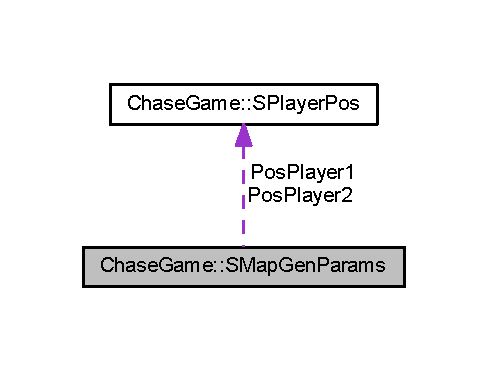
\includegraphics[width=234pt]{struct_chase_game_1_1_s_map_gen_params__coll__graph}
\end{center}
\end{figure}
\subsection*{Public Attributes}
\begin{DoxyCompactItemize}
\item 
\hypertarget{struct_chase_game_1_1_s_map_gen_params_a772c51dab66176dfe733e4e20cbf85d4}{unsigned \hyperlink{struct_chase_game_1_1_s_map_gen_params_a772c51dab66176dfe733e4e20cbf85d4}{Map\-Height} = 10}\label{struct_chase_game_1_1_s_map_gen_params_a772c51dab66176dfe733e4e20cbf85d4}

\begin{DoxyCompactList}\small\item\em Number of lines a map contains. \end{DoxyCompactList}\item 
\hypertarget{struct_chase_game_1_1_s_map_gen_params_a0897aeaa1a1a3a66697a6b441ca8c2de}{unsigned \hyperlink{struct_chase_game_1_1_s_map_gen_params_a0897aeaa1a1a3a66697a6b441ca8c2de}{Map\-Width} = 30}\label{struct_chase_game_1_1_s_map_gen_params_a0897aeaa1a1a3a66697a6b441ca8c2de}

\begin{DoxyCompactList}\small\item\em Number of columns a map contains. \end{DoxyCompactList}\item 
\hypertarget{struct_chase_game_1_1_s_map_gen_params_a8db28a9ee45a200d67b20fc803645501}{\hyperlink{struct_chase_game_1_1_s_player_pos}{S\-Player\-Pos} \hyperlink{struct_chase_game_1_1_s_map_gen_params_a8db28a9ee45a200d67b20fc803645501}{Pos\-Player1}}\label{struct_chase_game_1_1_s_map_gen_params_a8db28a9ee45a200d67b20fc803645501}

\begin{DoxyCompactList}\small\item\em Position of player one. \end{DoxyCompactList}\item 
\hypertarget{struct_chase_game_1_1_s_map_gen_params_afd0a0d4b22e228d547af88d38b6ae963}{\hyperlink{struct_chase_game_1_1_s_player_pos}{S\-Player\-Pos} \hyperlink{struct_chase_game_1_1_s_map_gen_params_afd0a0d4b22e228d547af88d38b6ae963}{Pos\-Player2}}\label{struct_chase_game_1_1_s_map_gen_params_afd0a0d4b22e228d547af88d38b6ae963}

\begin{DoxyCompactList}\small\item\em Position of player two. \end{DoxyCompactList}\end{DoxyCompactItemize}


\subsection{Detailed Description}
Contains all the map generation parameters. 

The documentation for this struct was generated from the following file\-:\begin{DoxyCompactItemize}
\item 
\hyperlink{globals_8hxx}{globals.\-hxx}\end{DoxyCompactItemize}

\hypertarget{struct_chase_game_1_1_s_player_keys}{\section{Chase\-Game\-:\-:S\-Player\-Keys Struct Reference}
\label{struct_chase_game_1_1_s_player_keys}\index{Chase\-Game\-::\-S\-Player\-Keys@{Chase\-Game\-::\-S\-Player\-Keys}}
}


Player specific keys.  




{\ttfamily \#include $<$globals.\-hxx$>$}

\subsection*{Public Attributes}
\begin{DoxyCompactItemize}
\item 
wchar\-\_\-t \hyperlink{struct_chase_game_1_1_s_player_keys_a0153d90bee31d3959e7a79377c4dd927}{Up}
\begin{DoxyCompactList}\small\item\em Up keycode. \end{DoxyCompactList}\item 
wchar\-\_\-t \hyperlink{struct_chase_game_1_1_s_player_keys_abe56af951c133c98b24401542f28ec9b}{Down}
\begin{DoxyCompactList}\small\item\em Down keycode. \end{DoxyCompactList}\item 
wchar\-\_\-t \hyperlink{struct_chase_game_1_1_s_player_keys_ab6c4f7e03fa43cd9443dcbd16a5e3250}{Left}
\begin{DoxyCompactList}\small\item\em Left keycode. \end{DoxyCompactList}\item 
wchar\-\_\-t \hyperlink{struct_chase_game_1_1_s_player_keys_a17ec0fea68ec78ad4577c6b56b83fa15}{Right}
\begin{DoxyCompactList}\small\item\em Right keycode. \end{DoxyCompactList}\end{DoxyCompactItemize}


\subsection{Detailed Description}
Player specific keys. 

Definition at line 81 of file globals.\-hxx.



\subsection{Member Data Documentation}
\hypertarget{struct_chase_game_1_1_s_player_keys_abe56af951c133c98b24401542f28ec9b}{\index{Chase\-Game\-::\-S\-Player\-Keys@{Chase\-Game\-::\-S\-Player\-Keys}!Down@{Down}}
\index{Down@{Down}!ChaseGame::SPlayerKeys@{Chase\-Game\-::\-S\-Player\-Keys}}
\subsubsection[{Down}]{\setlength{\rightskip}{0pt plus 5cm}wchar\-\_\-t Chase\-Game\-::\-S\-Player\-Keys\-::\-Down}}\label{struct_chase_game_1_1_s_player_keys_abe56af951c133c98b24401542f28ec9b}


Down keycode. 



Definition at line 85 of file globals.\-hxx.

\hypertarget{struct_chase_game_1_1_s_player_keys_ab6c4f7e03fa43cd9443dcbd16a5e3250}{\index{Chase\-Game\-::\-S\-Player\-Keys@{Chase\-Game\-::\-S\-Player\-Keys}!Left@{Left}}
\index{Left@{Left}!ChaseGame::SPlayerKeys@{Chase\-Game\-::\-S\-Player\-Keys}}
\subsubsection[{Left}]{\setlength{\rightskip}{0pt plus 5cm}wchar\-\_\-t Chase\-Game\-::\-S\-Player\-Keys\-::\-Left}}\label{struct_chase_game_1_1_s_player_keys_ab6c4f7e03fa43cd9443dcbd16a5e3250}


Left keycode. 



Definition at line 87 of file globals.\-hxx.

\hypertarget{struct_chase_game_1_1_s_player_keys_a17ec0fea68ec78ad4577c6b56b83fa15}{\index{Chase\-Game\-::\-S\-Player\-Keys@{Chase\-Game\-::\-S\-Player\-Keys}!Right@{Right}}
\index{Right@{Right}!ChaseGame::SPlayerKeys@{Chase\-Game\-::\-S\-Player\-Keys}}
\subsubsection[{Right}]{\setlength{\rightskip}{0pt plus 5cm}wchar\-\_\-t Chase\-Game\-::\-S\-Player\-Keys\-::\-Right}}\label{struct_chase_game_1_1_s_player_keys_a17ec0fea68ec78ad4577c6b56b83fa15}


Right keycode. 



Definition at line 89 of file globals.\-hxx.

\hypertarget{struct_chase_game_1_1_s_player_keys_a0153d90bee31d3959e7a79377c4dd927}{\index{Chase\-Game\-::\-S\-Player\-Keys@{Chase\-Game\-::\-S\-Player\-Keys}!Up@{Up}}
\index{Up@{Up}!ChaseGame::SPlayerKeys@{Chase\-Game\-::\-S\-Player\-Keys}}
\subsubsection[{Up}]{\setlength{\rightskip}{0pt plus 5cm}wchar\-\_\-t Chase\-Game\-::\-S\-Player\-Keys\-::\-Up}}\label{struct_chase_game_1_1_s_player_keys_a0153d90bee31d3959e7a79377c4dd927}


Up keycode. 



Definition at line 83 of file globals.\-hxx.



The documentation for this struct was generated from the following file\-:\begin{DoxyCompactItemize}
\item 
C\-:/\-Development/\-I\-U\-T/git -\/ Copie/projet/\hyperlink{globals_8hxx}{globals.\-hxx}\end{DoxyCompactItemize}

\hypertarget{struct_chase_game_1_1_s_player_pos}{\section{Chase\-Game\-:\-:S\-Player\-Pos Struct Reference}
\label{struct_chase_game_1_1_s_player_pos}\index{Chase\-Game\-::\-S\-Player\-Pos@{Chase\-Game\-::\-S\-Player\-Pos}}
}


Defines a position.  




{\ttfamily \#include $<$globals.\-hxx$>$}

\subsection*{Public Member Functions}
\begin{DoxyCompactItemize}
\item 
bool \hyperlink{struct_chase_game_1_1_s_player_pos_a16d84d116194f402b751f7265dd4fb91}{operator==} (const \hyperlink{struct_chase_game_1_1_s_player_pos}{S\-Player\-Pos} \&objet)
\begin{DoxyCompactList}\small\item\em Allow the comparison between to \hyperlink{struct_chase_game_1_1_s_player_pos}{S\-Player\-Pos}. \end{DoxyCompactList}\end{DoxyCompactItemize}
\subsection*{Public Attributes}
\begin{DoxyCompactItemize}
\item 
unsigned \hyperlink{struct_chase_game_1_1_s_player_pos_a28b353619ad10ef89da6308319b6ee39}{X} = 0
\begin{DoxyCompactList}\small\item\em X position. \end{DoxyCompactList}\item 
unsigned \hyperlink{struct_chase_game_1_1_s_player_pos_a0e20d9da2b1da89994a83e8acd72814c}{Y} = 0
\begin{DoxyCompactList}\small\item\em Y position. \end{DoxyCompactList}\end{DoxyCompactItemize}


\subsection{Detailed Description}
Defines a position. 

Definition at line 62 of file globals.\-hxx.



\subsection{Member Function Documentation}
\hypertarget{struct_chase_game_1_1_s_player_pos_a16d84d116194f402b751f7265dd4fb91}{\index{Chase\-Game\-::\-S\-Player\-Pos@{Chase\-Game\-::\-S\-Player\-Pos}!operator==@{operator==}}
\index{operator==@{operator==}!ChaseGame::SPlayerPos@{Chase\-Game\-::\-S\-Player\-Pos}}
\subsubsection[{operator==}]{\setlength{\rightskip}{0pt plus 5cm}bool Chase\-Game\-::\-S\-Player\-Pos\-::operator== (
\begin{DoxyParamCaption}
\item[{const {\bf S\-Player\-Pos} \&}]{objet}
\end{DoxyParamCaption}
)\hspace{0.3cm}{\ttfamily [inline]}}}\label{struct_chase_game_1_1_s_player_pos_a16d84d116194f402b751f7265dd4fb91}


Allow the comparison between to \hyperlink{struct_chase_game_1_1_s_player_pos}{S\-Player\-Pos}. 



Definition at line 69 of file globals.\-hxx.



\subsection{Member Data Documentation}
\hypertarget{struct_chase_game_1_1_s_player_pos_a28b353619ad10ef89da6308319b6ee39}{\index{Chase\-Game\-::\-S\-Player\-Pos@{Chase\-Game\-::\-S\-Player\-Pos}!X@{X}}
\index{X@{X}!ChaseGame::SPlayerPos@{Chase\-Game\-::\-S\-Player\-Pos}}
\subsubsection[{X}]{\setlength{\rightskip}{0pt plus 5cm}unsigned Chase\-Game\-::\-S\-Player\-Pos\-::\-X = 0}}\label{struct_chase_game_1_1_s_player_pos_a28b353619ad10ef89da6308319b6ee39}


X position. 



Definition at line 65 of file globals.\-hxx.

\hypertarget{struct_chase_game_1_1_s_player_pos_a0e20d9da2b1da89994a83e8acd72814c}{\index{Chase\-Game\-::\-S\-Player\-Pos@{Chase\-Game\-::\-S\-Player\-Pos}!Y@{Y}}
\index{Y@{Y}!ChaseGame::SPlayerPos@{Chase\-Game\-::\-S\-Player\-Pos}}
\subsubsection[{Y}]{\setlength{\rightskip}{0pt plus 5cm}unsigned Chase\-Game\-::\-S\-Player\-Pos\-::\-Y = 0}}\label{struct_chase_game_1_1_s_player_pos_a0e20d9da2b1da89994a83e8acd72814c}


Y position. 



Definition at line 67 of file globals.\-hxx.



The documentation for this struct was generated from the following file\-:\begin{DoxyCompactItemize}
\item 
C\-:/\-Development/\-I\-U\-T/git -\/ Copie/projet/\hyperlink{globals_8hxx}{globals.\-hxx}\end{DoxyCompactItemize}

\hypertarget{struct_chase_game_1_1_s_player_state}{\section{Chase\-Game\-:\-:S\-Player\-State Struct Reference}
\label{struct_chase_game_1_1_s_player_state}\index{Chase\-Game\-::\-S\-Player\-State@{Chase\-Game\-::\-S\-Player\-State}}
}


Player state.  




{\ttfamily \#include $<$globals.\-hxx$>$}



Collaboration diagram for Chase\-Game\-:\-:S\-Player\-State\-:
\nopagebreak
\begin{figure}[H]
\begin{center}
\leavevmode
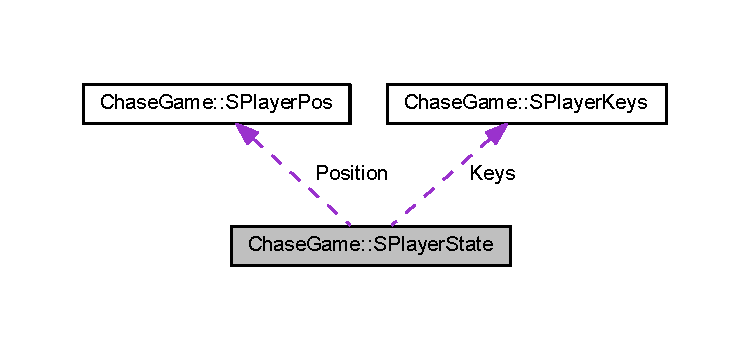
\includegraphics[width=350pt]{struct_chase_game_1_1_s_player_state__coll__graph}
\end{center}
\end{figure}
\subsection*{Public Attributes}
\begin{DoxyCompactItemize}
\item 
bool \hyperlink{struct_chase_game_1_1_s_player_state_acd7030969c414605901e551171078bb1}{Can\-Pass\-Through\-Walls}
\begin{DoxyCompactList}\small\item\em Can a player bypass wall collision check ? \end{DoxyCompactList}\item 
\hyperlink{struct_chase_game_1_1_s_player_pos}{S\-Player\-Pos} \hyperlink{struct_chase_game_1_1_s_player_state_a0a68b95a4255f2a543675f88b00847b4}{Position}
\begin{DoxyCompactList}\small\item\em Player position. \end{DoxyCompactList}\item 
\hyperlink{struct_chase_game_1_1_s_player_keys}{S\-Player\-Keys} \hyperlink{struct_chase_game_1_1_s_player_state_a3fc9ce0322ed28ff9c401983d91c69f2}{Keys}
\begin{DoxyCompactList}\small\item\em Keys specific to player. \end{DoxyCompactList}\item 
unsigned \hyperlink{struct_chase_game_1_1_s_player_state_a268594c795a70cf1eb9fe6061bfa57d0}{Score}
\begin{DoxyCompactList}\small\item\em Player score. \end{DoxyCompactList}\item 
bool \hyperlink{struct_chase_game_1_1_s_player_state_a2574de666d4744daefd7824b1c3c809f}{Is\-Chasing}
\begin{DoxyCompactList}\small\item\em Player role \-: chasing or being chased. \end{DoxyCompactList}\end{DoxyCompactItemize}


\subsection{Detailed Description}
Player state. 

\subsection{Member Data Documentation}
\hypertarget{struct_chase_game_1_1_s_player_state_acd7030969c414605901e551171078bb1}{\index{Chase\-Game\-::\-S\-Player\-State@{Chase\-Game\-::\-S\-Player\-State}!Can\-Pass\-Through\-Walls@{Can\-Pass\-Through\-Walls}}
\index{Can\-Pass\-Through\-Walls@{Can\-Pass\-Through\-Walls}!ChaseGame::SPlayerState@{Chase\-Game\-::\-S\-Player\-State}}
\subsubsection[{Can\-Pass\-Through\-Walls}]{\setlength{\rightskip}{0pt plus 5cm}bool Chase\-Game\-::\-S\-Player\-State\-::\-Can\-Pass\-Through\-Walls}}\label{struct_chase_game_1_1_s_player_state_acd7030969c414605901e551171078bb1}


Can a player bypass wall collision check ? 

\hypertarget{struct_chase_game_1_1_s_player_state_a2574de666d4744daefd7824b1c3c809f}{\index{Chase\-Game\-::\-S\-Player\-State@{Chase\-Game\-::\-S\-Player\-State}!Is\-Chasing@{Is\-Chasing}}
\index{Is\-Chasing@{Is\-Chasing}!ChaseGame::SPlayerState@{Chase\-Game\-::\-S\-Player\-State}}
\subsubsection[{Is\-Chasing}]{\setlength{\rightskip}{0pt plus 5cm}bool Chase\-Game\-::\-S\-Player\-State\-::\-Is\-Chasing}}\label{struct_chase_game_1_1_s_player_state_a2574de666d4744daefd7824b1c3c809f}


Player role \-: chasing or being chased. 

\hypertarget{struct_chase_game_1_1_s_player_state_a3fc9ce0322ed28ff9c401983d91c69f2}{\index{Chase\-Game\-::\-S\-Player\-State@{Chase\-Game\-::\-S\-Player\-State}!Keys@{Keys}}
\index{Keys@{Keys}!ChaseGame::SPlayerState@{Chase\-Game\-::\-S\-Player\-State}}
\subsubsection[{Keys}]{\setlength{\rightskip}{0pt plus 5cm}{\bf S\-Player\-Keys} Chase\-Game\-::\-S\-Player\-State\-::\-Keys}}\label{struct_chase_game_1_1_s_player_state_a3fc9ce0322ed28ff9c401983d91c69f2}


Keys specific to player. 

\hypertarget{struct_chase_game_1_1_s_player_state_a0a68b95a4255f2a543675f88b00847b4}{\index{Chase\-Game\-::\-S\-Player\-State@{Chase\-Game\-::\-S\-Player\-State}!Position@{Position}}
\index{Position@{Position}!ChaseGame::SPlayerState@{Chase\-Game\-::\-S\-Player\-State}}
\subsubsection[{Position}]{\setlength{\rightskip}{0pt plus 5cm}{\bf S\-Player\-Pos} Chase\-Game\-::\-S\-Player\-State\-::\-Position}}\label{struct_chase_game_1_1_s_player_state_a0a68b95a4255f2a543675f88b00847b4}


Player position. 

\hypertarget{struct_chase_game_1_1_s_player_state_a268594c795a70cf1eb9fe6061bfa57d0}{\index{Chase\-Game\-::\-S\-Player\-State@{Chase\-Game\-::\-S\-Player\-State}!Score@{Score}}
\index{Score@{Score}!ChaseGame::SPlayerState@{Chase\-Game\-::\-S\-Player\-State}}
\subsubsection[{Score}]{\setlength{\rightskip}{0pt plus 5cm}unsigned Chase\-Game\-::\-S\-Player\-State\-::\-Score}}\label{struct_chase_game_1_1_s_player_state_a268594c795a70cf1eb9fe6061bfa57d0}


Player score. 



The documentation for this struct was generated from the following file\-:\begin{DoxyCompactItemize}
\item 
\hyperlink{globals_8hxx}{globals.\-hxx}\end{DoxyCompactItemize}

\chapter{File Documentation}
\hypertarget{audio_8cxx}{\section{C\-:/\-Development/\-I\-U\-T/git -\/ Copie/projet/audio.cxx File Reference}
\label{audio_8cxx}\index{C\-:/\-Development/\-I\-U\-T/git -\/ Copie/projet/audio.\-cxx@{C\-:/\-Development/\-I\-U\-T/git -\/ Copie/projet/audio.\-cxx}}
}
{\ttfamily \#include $<$iostream$>$}\\*
{\ttfamily \#include $<$string$>$}\\*
{\ttfamily \#include $<$vector$>$}\\*
{\ttfamily \#include $<$limits$>$}\\*
{\ttfamily \#include $<$time.\-h$>$}\\*
{\ttfamily \#include $<$stdlib.\-h$>$}\\*
{\ttfamily \#include $<$map$>$}\\*
{\ttfamily \#include $<$S\-F\-M\-L/\-System.\-hpp$>$}\\*
{\ttfamily \#include $<$S\-F\-M\-L/\-Audio.\-hpp$>$}\\*
{\ttfamily \#include \char`\"{}globals.\-hxx\char`\"{}}\\*
{\ttfamily \#include \char`\"{}audio.\-hxx\char`\"{}}\\*
Include dependency graph for audio.\-cxx\-:\nopagebreak
\begin{figure}[H]
\begin{center}
\leavevmode
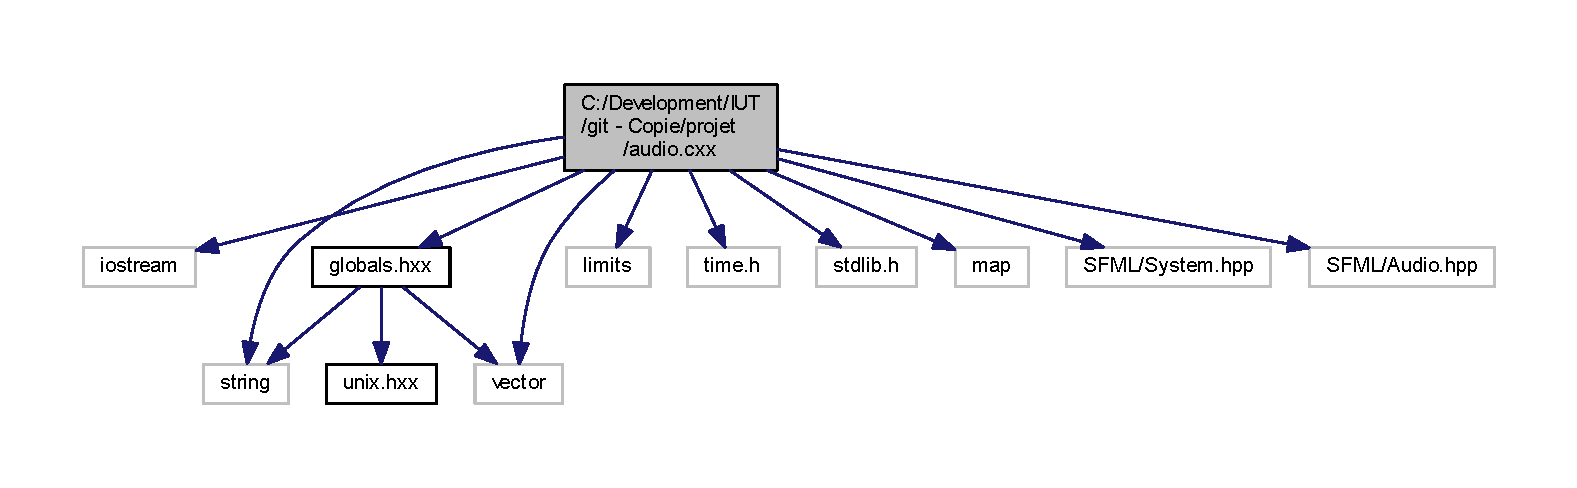
\includegraphics[width=350pt]{audio_8cxx__incl}
\end{center}
\end{figure}
\subsection*{Namespaces}
\begin{DoxyCompactItemize}
\item 
\hyperlink{namespace_chase_game}{Chase\-Game}
\begin{DoxyCompactList}\small\item\em Main namespace Project namespace for the game Contains all the funcitons, structs, enums and constansts related to the game. \end{DoxyCompactList}\end{DoxyCompactItemize}
\subsection*{Functions}
\begin{DoxyCompactItemize}
\item 
void \hyperlink{namespace_chase_game_af423e47c7318b7eeb67ff1f1a6b1547d}{Chase\-Game\-::\-Set\-Game\-State} (map$<$ string, sf\-::\-Music \& $>$ \&Tracks, int Game\-State, bool Do\-Fade)
\item 
void \hyperlink{namespace_chase_game_af1b7d4727ff31281f8efdf46175e94c3}{Chase\-Game\-::\-Init\-Songs} (sf\-::\-Music \&Track1\-A, sf\-::\-Music \&Track1\-B, sf\-::\-Music \&Track1\-C, sf\-::\-Music \&Track2)
\begin{DoxyCompactList}\small\item\em Loads the songs and inits them. \end{DoxyCompactList}\item 
void \hyperlink{namespace_chase_game_a1fafa6862bb2df06c93d286361fefaa4}{Chase\-Game\-::\-Double\-Song\-Volume\-Fading} (sf\-::\-Music \&A, sf\-::\-Music \&B, float Volume\-A, float Volume\-B, float Fade\-Duration)
\begin{DoxyCompactList}\small\item\em Do a crossface between two songs. \end{DoxyCompactList}\item 
void \hyperlink{namespace_chase_game_a3b9e1d486d981f5332d23142eb4777b7}{Chase\-Game\-::\-Triple\-Song\-Volume\-Fading} (sf\-::\-Music \&A, sf\-::\-Music \&B, sf\-::\-Music \&C, float Volume\-A, float Volume\-B, float Volume\-C, float Fade\-Duration)
\begin{DoxyCompactList}\small\item\em Do a crossface between three song. \end{DoxyCompactList}\end{DoxyCompactItemize}

\hypertarget{audio_8hxx}{\section{C\-:/\-Development/\-I\-U\-T/git -\/ Copie/projet/audio.hxx File Reference}
\label{audio_8hxx}\index{C\-:/\-Development/\-I\-U\-T/git -\/ Copie/projet/audio.\-hxx@{C\-:/\-Development/\-I\-U\-T/git -\/ Copie/projet/audio.\-hxx}}
}


\hyperlink{audio_8cxx}{audio.\-cxx} function prototypes  


{\ttfamily \#include $<$S\-F\-M\-L/\-System.\-hpp$>$}\\*
{\ttfamily \#include $<$S\-F\-M\-L/\-Audio.\-hpp$>$}\\*
{\ttfamily \#include $<$string$>$}\\*
{\ttfamily \#include $<$map$>$}\\*
{\ttfamily \#include \char`\"{}globals.\-hxx\char`\"{}}\\*
Include dependency graph for audio.\-hxx\-:\nopagebreak
\begin{figure}[H]
\begin{center}
\leavevmode
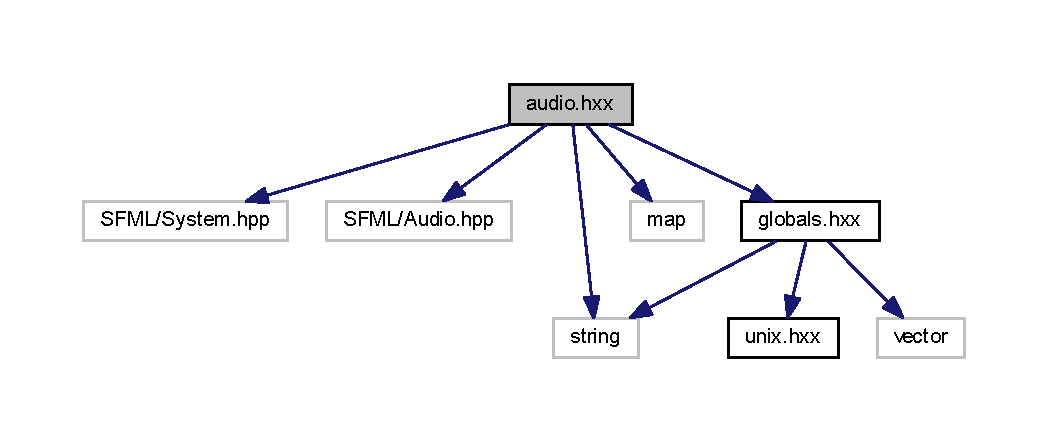
\includegraphics[width=350pt]{audio_8hxx__incl}
\end{center}
\end{figure}
This graph shows which files directly or indirectly include this file\-:\nopagebreak
\begin{figure}[H]
\begin{center}
\leavevmode
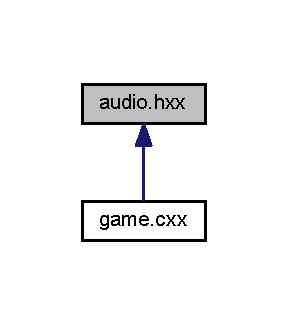
\includegraphics[width=182pt]{audio_8hxx__dep__incl}
\end{center}
\end{figure}
\subsection*{Namespaces}
\begin{DoxyCompactItemize}
\item 
\hyperlink{namespace_chase_game}{Chase\-Game}
\end{DoxyCompactItemize}
\subsection*{Functions}
\begin{DoxyCompactItemize}
\item 
void \hyperlink{namespace_chase_game_a5aeec1309079c5c64aec0fd24a4b17c1}{Chase\-Game\-::\-Set\-Game\-State} (std\-::map$<$ std\-::string, sf\-::\-Music \& $>$ \&Tracks, int Game\-State)
\begin{DoxyCompactList}\small\item\em Sets music volumes according to the game state. \end{DoxyCompactList}\end{DoxyCompactItemize}


\subsection{Detailed Description}
\hyperlink{audio_8cxx}{audio.\-cxx} function prototypes \begin{DoxyAuthor}{Author}

\end{DoxyAuthor}
\begin{DoxyDate}{Date}
09/01/14 
\end{DoxyDate}
\begin{DoxyVersion}{Version}
1 
\end{DoxyVersion}


Definition in file \hyperlink{audio_8hxx_source}{audio.\-hxx}.


\hypertarget{banana_8cxx}{\section{banana.\-cxx File Reference}
\label{banana_8cxx}\index{banana.\-cxx@{banana.\-cxx}}
}


Super Banana !  


{\ttfamily \#include $<$iostream$>$}\\*
{\ttfamily \#include $<$S\-F\-M\-L/\-System.\-hpp$>$}\\*
{\ttfamily \#include $<$S\-F\-M\-L/\-Audio.\-hpp$>$}\\*
{\ttfamily \#include \char`\"{}globals.\-hxx\char`\"{}}\\*
{\ttfamily \#include \char`\"{}unix.\-hxx\char`\"{}}\\*
Include dependency graph for banana.\-cxx\-:
\nopagebreak
\begin{figure}[H]
\begin{center}
\leavevmode
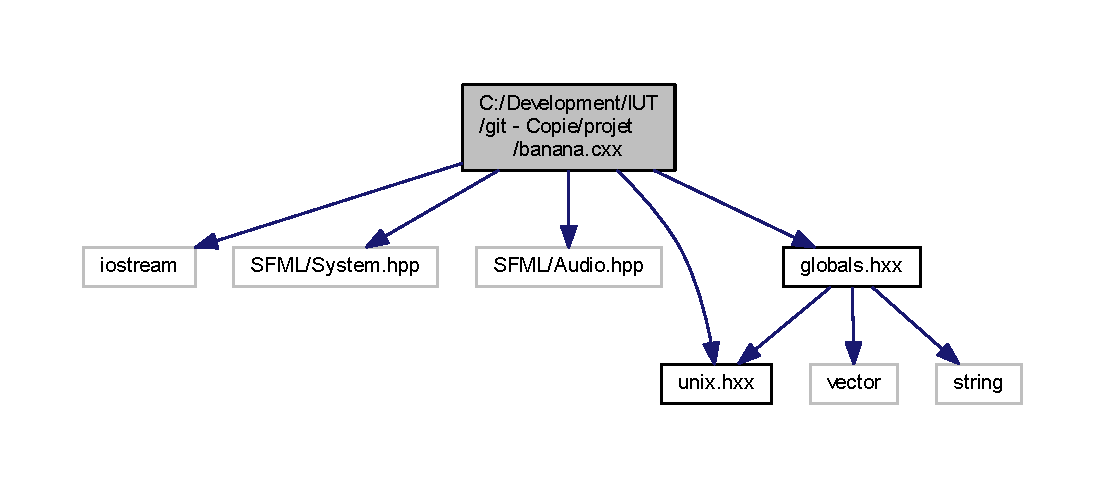
\includegraphics[width=350pt]{banana_8cxx__incl}
\end{center}
\end{figure}
\subsection*{Namespaces}
\begin{DoxyCompactItemize}
\item 
\hyperlink{namespace_chase_game}{Chase\-Game}
\begin{DoxyCompactList}\small\item\em Main namespace Project namespace for the game Contains all the funcitons, structs, enums and constansts related to the game. \end{DoxyCompactList}\end{DoxyCompactItemize}
\subsection*{Functions}
\begin{DoxyCompactItemize}
\item 
\hypertarget{namespace_chase_game_a19b95183bbaf6684ffc6511a4f9922f5}{void {\bfseries Chase\-Game\-::\-Super\-Banana} ()}\label{namespace_chase_game_a19b95183bbaf6684ffc6511a4f9922f5}

\end{DoxyCompactItemize}


\subsection{Detailed Description}
Super Banana ! \begin{DoxyAuthor}{Author}
Nazim'n'Josh 
\end{DoxyAuthor}
\begin{DoxyDate}{Date}
10/01/14 
\end{DoxyDate}
\begin{DoxyVersion}{Version}
1
\end{DoxyVersion}
Contains functions for the launching of Ariane V 
\hypertarget{banana_8hxx}{\section{banana.\-hxx File Reference}
\label{banana_8hxx}\index{banana.\-hxx@{banana.\-hxx}}
}


\hyperlink{banana_8cxx}{banana.\-cxx} function prototypes  


This graph shows which files directly or indirectly include this file\-:\nopagebreak
\begin{figure}[H]
\begin{center}
\leavevmode
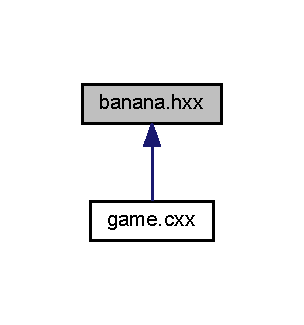
\includegraphics[width=146pt]{banana_8hxx__dep__incl}
\end{center}
\end{figure}
\subsection*{Namespaces}
\begin{DoxyCompactItemize}
\item 
\hyperlink{namespace_chase_game}{Chase\-Game}
\begin{DoxyCompactList}\small\item\em Main namespace Project namespace for the game Contains all the funcitons, structs, enums and constansts related to the game. \end{DoxyCompactList}\end{DoxyCompactItemize}
\subsection*{Functions}
\begin{DoxyCompactItemize}
\item 
void \hyperlink{namespace_chase_game_a19b95183bbaf6684ffc6511a4f9922f5}{Chase\-Game\-::\-Super\-Banana} ()
\end{DoxyCompactItemize}


\subsection{Detailed Description}
\hyperlink{banana_8cxx}{banana.\-cxx} function prototypes \begin{DoxyAuthor}{Author}
Nazim'n'Josh 
\end{DoxyAuthor}
\begin{DoxyDate}{Date}
10/01/14 
\end{DoxyDate}
\begin{DoxyVersion}{Version}
1 
\end{DoxyVersion}

\hypertarget{bonus_8cxx}{\section{bonus.\-cxx File Reference}
\label{bonus_8cxx}\index{bonus.\-cxx@{bonus.\-cxx}}
}


File related bonus and malus.  


{\ttfamily \#include $<$iostream$>$}\\*
{\ttfamily \#include $<$fstream$>$}\\*
{\ttfamily \#include $<$string$>$}\\*
{\ttfamily \#include $<$vector$>$}\\*
{\ttfamily \#include \char`\"{}globals.\-hxx\char`\"{}}\\*
{\ttfamily \#include \char`\"{}map.\-hxx\char`\"{}}\\*
Include dependency graph for bonus.\-cxx\-:\nopagebreak
\begin{figure}[H]
\begin{center}
\leavevmode
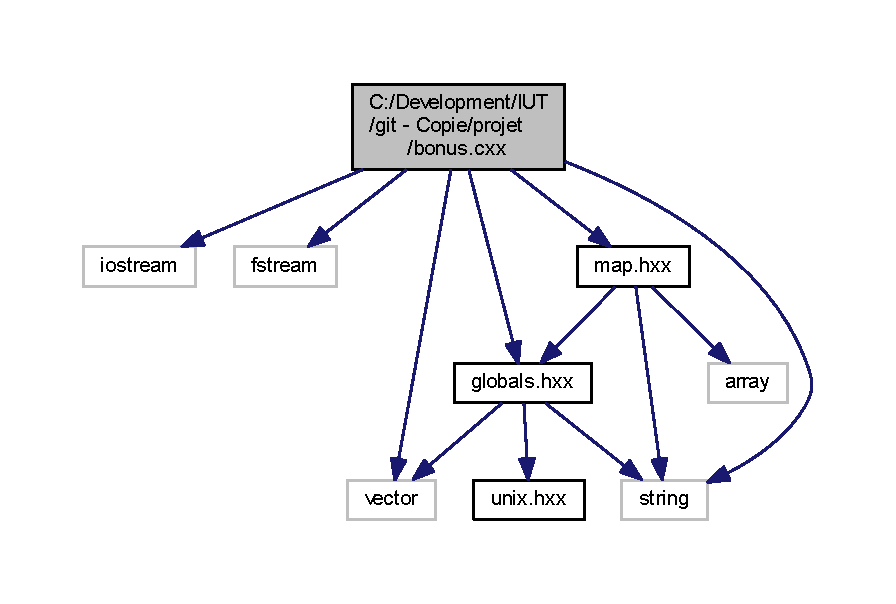
\includegraphics[width=350pt]{bonus_8cxx__incl}
\end{center}
\end{figure}
\subsection*{Namespaces}
\begin{DoxyCompactItemize}
\item 
\hyperlink{namespace_chase_game}{Chase\-Game}
\begin{DoxyCompactList}\small\item\em Main namespace Project namespace for the game Contains all the funcitons, structs, enums and constansts related to the game. \end{DoxyCompactList}\end{DoxyCompactItemize}
\subsection*{Functions}
\begin{DoxyCompactItemize}
\item 
\hypertarget{namespace_chase_game_aee2df7cbf4974e167612a7415943f3b0}{unsigned {\bfseries Chase\-Game\-::\-R\-Rand} (unsigned Min, unsigned Max)}\label{namespace_chase_game_aee2df7cbf4974e167612a7415943f3b0}

\item 
\hypertarget{namespace_chase_game_a831cfcb5623ab30034f57cbfff28c720}{void {\bfseries Chase\-Game\-::\-Gen\-Bonus\-\_\-\-Malus} (C\-Matrix \&Mat)}\label{namespace_chase_game_a831cfcb5623ab30034f57cbfff28c720}

\item 
\hypertarget{namespace_chase_game_a0e3e15bf28c7e96d0ba0bd14094ba71f}{void {\bfseries Chase\-Game\-::\-Effect} (C\-Matrix \&Mat, S\-Player\-Pos Player)}\label{namespace_chase_game_a0e3e15bf28c7e96d0ba0bd14094ba71f}

\end{DoxyCompactItemize}


\subsection{Detailed Description}
File related bonus and malus. \begin{DoxyAuthor}{Author}

\end{DoxyAuthor}
\begin{DoxyDate}{Date}
10/01/14 
\end{DoxyDate}
\begin{DoxyVersion}{Version}
1
\end{DoxyVersion}
Contains functions that creates bonuses and maluses in the map 
\hypertarget{bonus_8hxx}{\section{C\-:/\-Development/\-I\-U\-T/git -\/ Copie/projet/bonus.hxx File Reference}
\label{bonus_8hxx}\index{C\-:/\-Development/\-I\-U\-T/git -\/ Copie/projet/bonus.\-hxx@{C\-:/\-Development/\-I\-U\-T/git -\/ Copie/projet/bonus.\-hxx}}
}


\hyperlink{bonus_8cxx}{bonus.\-cxx} function prototypes  


{\ttfamily \#include $<$string$>$}\\*
{\ttfamily \#include \char`\"{}globals.\-hxx\char`\"{}}\\*
Include dependency graph for bonus.\-hxx\-:\nopagebreak
\begin{figure}[H]
\begin{center}
\leavevmode
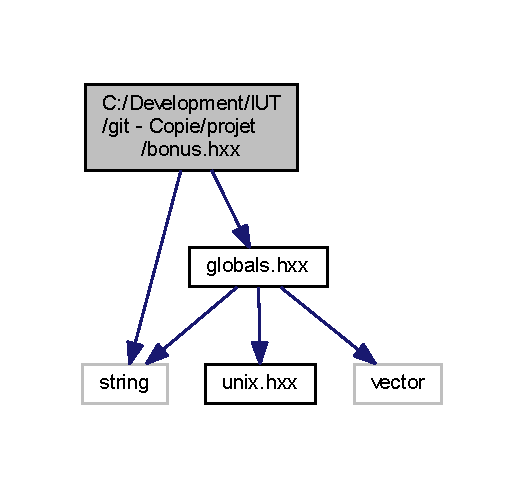
\includegraphics[width=252pt]{bonus_8hxx__incl}
\end{center}
\end{figure}
\subsection*{Namespaces}
\begin{DoxyCompactItemize}
\item 
\hyperlink{namespace_chase_game}{Chase\-Game}
\begin{DoxyCompactList}\small\item\em Main namespace Project namespace for the game Contains all the funcitons, structs, enums and constansts related to the game. \end{DoxyCompactList}\end{DoxyCompactItemize}
\subsection*{Functions}
\begin{DoxyCompactItemize}
\item 
unsigned \hyperlink{namespace_chase_game_aee2df7cbf4974e167612a7415943f3b0}{Chase\-Game\-::\-R\-Rand} (unsigned Min, unsigned Max)
\item 
void \hyperlink{namespace_chase_game_a831cfcb5623ab30034f57cbfff28c720}{Chase\-Game\-::\-Gen\-Bonus\-\_\-\-Malus} (C\-Matrix \&Mat)
\item 
void \hyperlink{namespace_chase_game_a0e3e15bf28c7e96d0ba0bd14094ba71f}{Chase\-Game\-::\-Effect} (C\-Matrix \&Mat, S\-Player\-Pos Player)
\end{DoxyCompactItemize}


\subsection{Detailed Description}
\hyperlink{bonus_8cxx}{bonus.\-cxx} function prototypes \begin{DoxyAuthor}{Author}

\end{DoxyAuthor}
\begin{DoxyDate}{Date}
10/01/14 
\end{DoxyDate}
\begin{DoxyVersion}{Version}
1 
\end{DoxyVersion}


Definition in file \hyperlink{bonus_8hxx_source}{bonus.\-hxx}.


\hypertarget{_c_h_a_n_g_e_s_8md}{\section{C\-H\-A\-N\-G\-E\-S.\-md File Reference}
\label{_c_h_a_n_g_e_s_8md}\index{C\-H\-A\-N\-G\-E\-S.\-md@{C\-H\-A\-N\-G\-E\-S.\-md}}
}

\hypertarget{file_8cxx}{\section{file.\-cxx File Reference}
\label{file_8cxx}\index{file.\-cxx@{file.\-cxx}}
}


File related functions.  


{\ttfamily \#include $<$iostream$>$}\\*
{\ttfamily \#include $<$fstream$>$}\\*
{\ttfamily \#include $<$string$>$}\\*
{\ttfamily \#include \char`\"{}globals.\-hxx\char`\"{}}\\*
{\ttfamily \#include \char`\"{}file.\-hxx\char`\"{}}\\*
Include dependency graph for file.\-cxx\-:\nopagebreak
\begin{figure}[H]
\begin{center}
\leavevmode
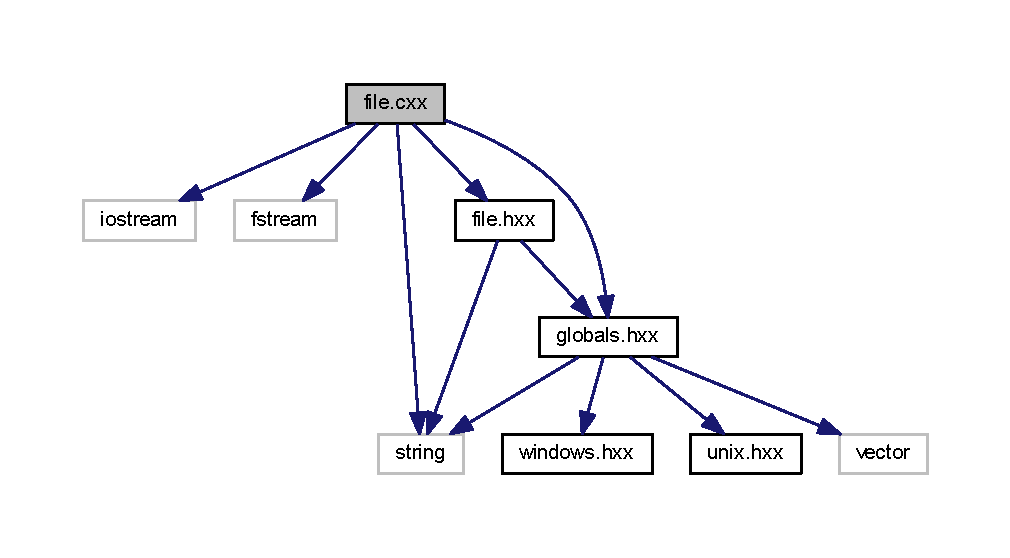
\includegraphics[width=350pt]{file_8cxx__incl}
\end{center}
\end{figure}
\subsection*{Namespaces}
\begin{DoxyCompactItemize}
\item 
\hyperlink{namespace_chase_game}{Chase\-Game}
\begin{DoxyCompactList}\small\item\em Main namespace Project namespace for the game Contains all the funcitons, structs, enums and constansts related to the game. \end{DoxyCompactList}\end{DoxyCompactItemize}
\subsection*{Functions}
\begin{DoxyCompactItemize}
\item 
S\-Map\-Gen\-Params \hyperlink{namespace_chase_game_a4779af792d3de8e274049bf2019e0343}{Chase\-Game\-::\-Load\-Map\-Gen\-Config} (const string \&File\-Name)
\item 
bool \hyperlink{namespace_chase_game_a98e8d90127c802c1445266e39966c3fb}{Chase\-Game\-::\-Save\-Map\-Config} (const string \&File\-Name, S\-Map\-Gen\-Params \&Params)
\item 
S\-Game\-Status \hyperlink{namespace_chase_game_addd460052ec5a5fe3010665ca84b07ec}{Chase\-Game\-::\-Load\-Game\-Config} (const std\-::string \&File\-Name)
\begin{DoxyCompactList}\small\item\em Loads game configuration. \end{DoxyCompactList}\item 
bool \hyperlink{namespace_chase_game_a39f8b039151b1a3eef82fdc1c6f52091}{Chase\-Game\-::\-Save\-Game\-Config} (const string \&File\-Name, S\-Game\-Status \&Config)
\end{DoxyCompactItemize}


\subsection{Detailed Description}
File related functions. \begin{DoxyAuthor}{Author}

\end{DoxyAuthor}
\begin{DoxyDate}{Date}
08/01/14 
\end{DoxyDate}
\begin{DoxyVersion}{Version}
1
\end{DoxyVersion}
Contains functions that loads or save config files 
\hypertarget{file_8hxx}{\section{C\-:/\-Development/\-I\-U\-T/git -\/ Copie/projet/file.hxx File Reference}
\label{file_8hxx}\index{C\-:/\-Development/\-I\-U\-T/git -\/ Copie/projet/file.\-hxx@{C\-:/\-Development/\-I\-U\-T/git -\/ Copie/projet/file.\-hxx}}
}


\hyperlink{file_8cxx}{file.\-cxx} function prototypes  


{\ttfamily \#include $<$string$>$}\\*
{\ttfamily \#include \char`\"{}globals.\-hxx\char`\"{}}\\*
Include dependency graph for file.\-hxx\-:
\nopagebreak
\begin{figure}[H]
\begin{center}
\leavevmode
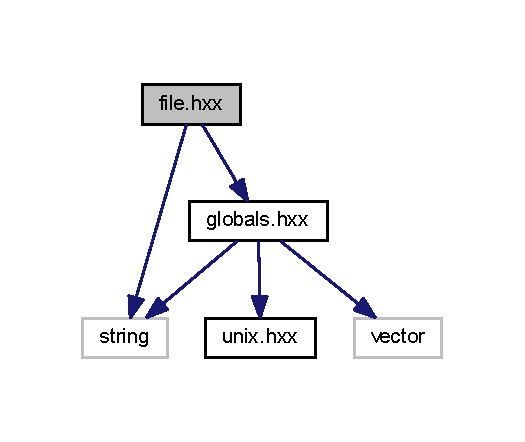
\includegraphics[width=252pt]{file_8hxx__incl}
\end{center}
\end{figure}
This graph shows which files directly or indirectly include this file\-:
\nopagebreak
\begin{figure}[H]
\begin{center}
\leavevmode
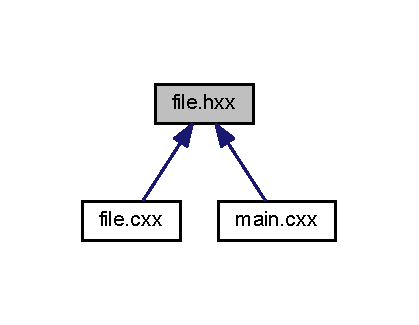
\includegraphics[width=350pt]{file_8hxx__dep__incl}
\end{center}
\end{figure}
\subsection*{Namespaces}
\begin{DoxyCompactItemize}
\item 
\hyperlink{namespace_chase_game}{Chase\-Game}
\end{DoxyCompactItemize}
\subsection*{Functions}
\begin{DoxyCompactItemize}
\item 
S\-Map\-Gen\-Params \hyperlink{namespace_chase_game_a9c5b5d91cb4251cae461faa4ace8a0cf}{Chase\-Game\-::\-Load\-Map\-Gen\-Config} (const std\-::string \&File\-Name)
\begin{DoxyCompactList}\small\item\em Loads parameters from a config file. \end{DoxyCompactList}\item 
bool \hyperlink{namespace_chase_game_a4c62f61c6aac5bf06292aa51294fd211}{Chase\-Game\-::\-Save\-Map\-Config} (const std\-::string \&File\-Name, S\-Map\-Gen\-Params \&Params)
\begin{DoxyCompactList}\small\item\em Saves parameters in a config file. \end{DoxyCompactList}\item 
S\-Game\-Status \hyperlink{namespace_chase_game_addd460052ec5a5fe3010665ca84b07ec}{Chase\-Game\-::\-Load\-Game\-Config} (const std\-::string \&File\-Name)
\begin{DoxyCompactList}\small\item\em Loads game configuration. \end{DoxyCompactList}\item 
bool \hyperlink{namespace_chase_game_a561c85a018e34c8baa21f7f500a3c9c7}{Chase\-Game\-::\-Save\-Game\-Config} (const std\-::string \&File\-Name, S\-Game\-Status \&Config)
\begin{DoxyCompactList}\small\item\em Saves game configuration in a config file. \end{DoxyCompactList}\end{DoxyCompactItemize}


\subsection{Detailed Description}
\hyperlink{file_8cxx}{file.\-cxx} function prototypes \begin{DoxyAuthor}{Author}

\end{DoxyAuthor}
\begin{DoxyDate}{Date}
08/01/14 
\end{DoxyDate}
\begin{DoxyVersion}{Version}
1 
\end{DoxyVersion}


Definition in file \hyperlink{file_8hxx_source}{file.\-hxx}.


\hypertarget{game_8cxx}{\section{C\-:/\-Development/\-I\-U\-T/git -\/ Copie/projet/game.cxx File Reference}
\label{game_8cxx}\index{C\-:/\-Development/\-I\-U\-T/git -\/ Copie/projet/game.\-cxx@{C\-:/\-Development/\-I\-U\-T/git -\/ Copie/projet/game.\-cxx}}
}


Audio related functions.  


{\ttfamily \#include $<$iostream$>$}\\*
{\ttfamily \#include $<$string$>$}\\*
{\ttfamily \#include $<$vector$>$}\\*
{\ttfamily \#include $<$limits$>$}\\*
{\ttfamily \#include $<$map$>$}\\*
{\ttfamily \#include $<$time.\-h$>$}\\*
{\ttfamily \#include $<$stdlib.\-h$>$}\\*
{\ttfamily \#include $<$S\-F\-M\-L/\-System.\-hpp$>$}\\*
{\ttfamily \#include $<$S\-F\-M\-L/\-Audio.\-hpp$>$}\\*
{\ttfamily \#include \char`\"{}globals.\-hxx\char`\"{}}\\*
{\ttfamily \#include \char`\"{}unix.\-hxx\char`\"{}}\\*
{\ttfamily \#include \char`\"{}file.\-hxx\char`\"{}}\\*
{\ttfamily \#include \char`\"{}map.\-hxx\char`\"{}}\\*
{\ttfamily \#include \char`\"{}audio.\-hxx\char`\"{}}\\*
Include dependency graph for game.\-cxx\-:\nopagebreak
\begin{figure}[H]
\begin{center}
\leavevmode
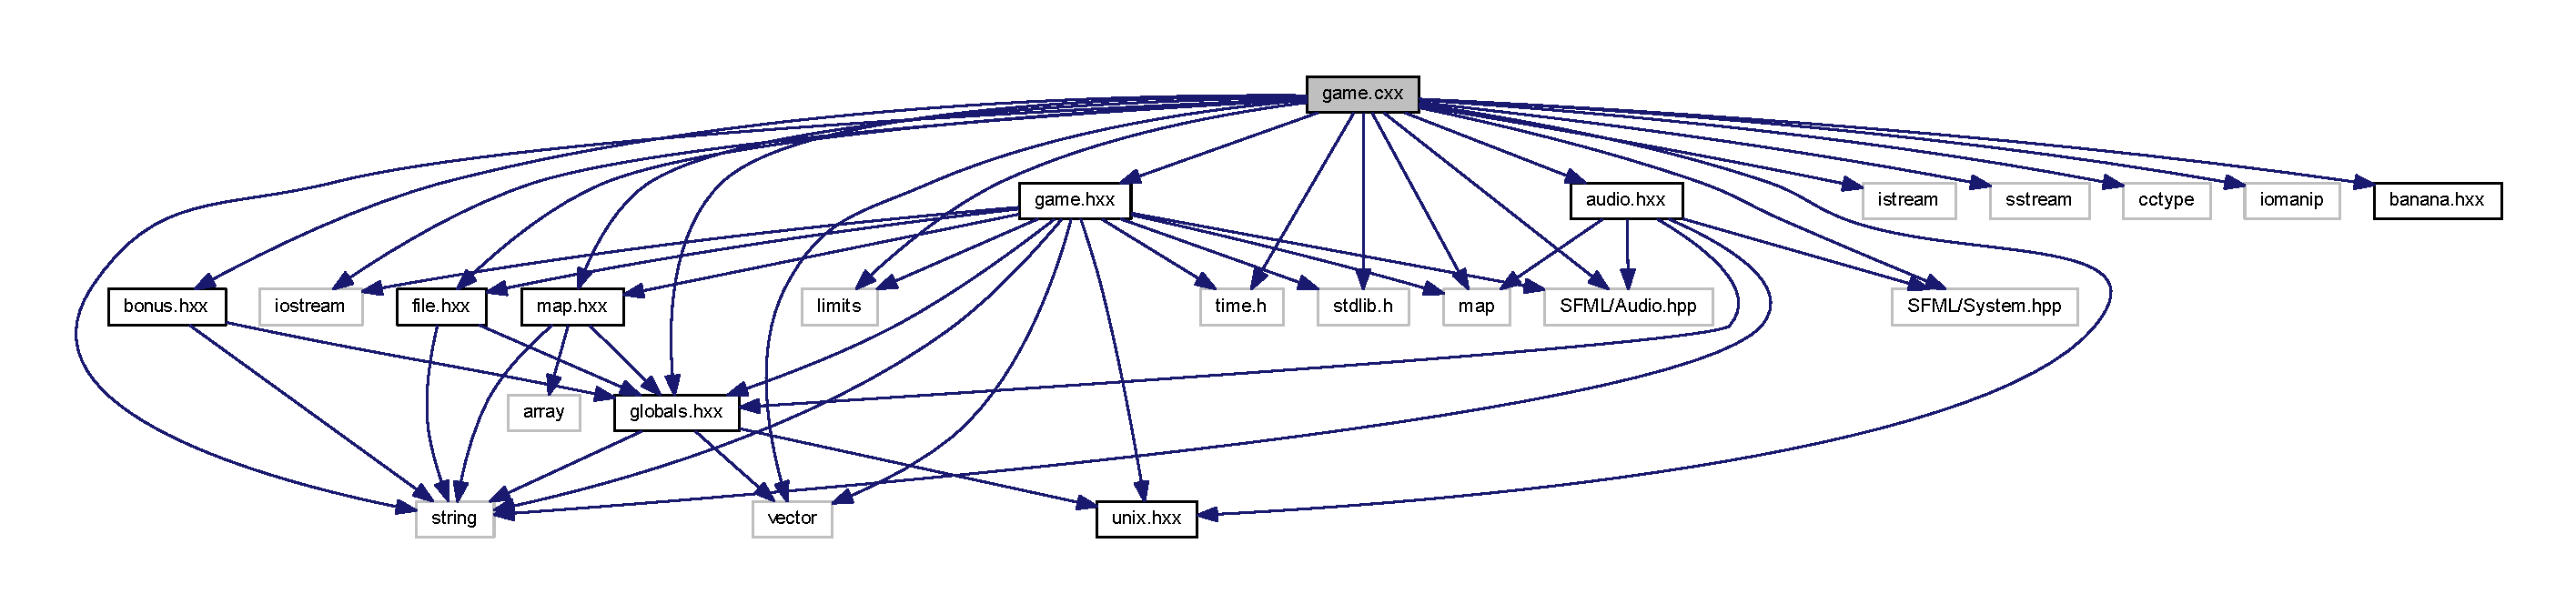
\includegraphics[width=350pt]{game_8cxx__incl}
\end{center}
\end{figure}
\subsection*{Namespaces}
\begin{DoxyCompactItemize}
\item 
\hyperlink{namespace_chase_game}{Chase\-Game}
\end{DoxyCompactItemize}
\subsection*{Functions}
\begin{DoxyCompactItemize}
\item 
char \hyperlink{namespace_chase_game_ab5112517855da810fe3b7bdb81d58484}{Chase\-Game\-::\-Process\-Input} (C\-Matrix \&Mat, const char Input, S\-Game\-Status \&Config)
\begin{DoxyCompactList}\small\item\em Processes user input. \end{DoxyCompactList}\item 
bool \hyperlink{namespace_chase_game_acb136d1f2b7073d2dc61bc2e2d65b931}{Chase\-Game\-::\-Game\-Round\-Loop} (C\-Matrix \&Mat, S\-Map\-Gen\-Params \&Map\-Gen\-Params, S\-Game\-Status \&Game\-Status)
\item 
void \hyperlink{namespace_chase_game_aaaedf9429ec62c336f4324d580eec51c}{Chase\-Game\-::\-Pause} ()
\item 
bool \hyperlink{namespace_chase_game_a1ca6f3f9092b35d9bea0343fd032d7f0}{Chase\-Game\-::\-Game\-Loop} (S\-Map\-Gen\-Params \&Map\-Gen\-Params, S\-Game\-Status \&Game\-Status, map$<$ string, sf\-::\-Music \& $>$ \&Music)
\item 
void \hyperlink{namespace_chase_game_a528073d13296b3cf84a6ae07c3550e74}{Chase\-Game\-::\-Start\-Game} ()
\begin{DoxyCompactList}\small\item\em This function starts the game. \end{DoxyCompactList}\end{DoxyCompactItemize}


\subsection{Detailed Description}
Audio related functions. Gameplay related functions.

\begin{DoxyAuthor}{Author}

\end{DoxyAuthor}
\begin{DoxyDate}{Date}
09/01/14 
\end{DoxyDate}
\begin{DoxyVersion}{Version}
1 
\end{DoxyVersion}


Definition in file \hyperlink{game_8cxx_source}{game.\-cxx}.


\hypertarget{game_8hxx}{\section{C\-:/\-Development/\-I\-U\-T/git -\/ Copie/projet/game.hxx File Reference}
\label{game_8hxx}\index{C\-:/\-Development/\-I\-U\-T/git -\/ Copie/projet/game.\-hxx@{C\-:/\-Development/\-I\-U\-T/git -\/ Copie/projet/game.\-hxx}}
}


\hyperlink{game_8cxx}{game.\-cxx} function prototypes  


{\ttfamily \#include $<$iostream$>$}\\*
{\ttfamily \#include $<$string$>$}\\*
{\ttfamily \#include $<$vector$>$}\\*
{\ttfamily \#include $<$limits$>$}\\*
{\ttfamily \#include $<$time.\-h$>$}\\*
{\ttfamily \#include $<$stdlib.\-h$>$}\\*
{\ttfamily \#include $<$map$>$}\\*
{\ttfamily \#include $<$S\-F\-M\-L/\-Audio.\-hpp$>$}\\*
{\ttfamily \#include \char`\"{}globals.\-hxx\char`\"{}}\\*
{\ttfamily \#include \char`\"{}unix.\-hxx\char`\"{}}\\*
{\ttfamily \#include \char`\"{}file.\-hxx\char`\"{}}\\*
{\ttfamily \#include \char`\"{}map.\-hxx\char`\"{}}\\*
Include dependency graph for game.\-hxx\-:\nopagebreak
\begin{figure}[H]
\begin{center}
\leavevmode
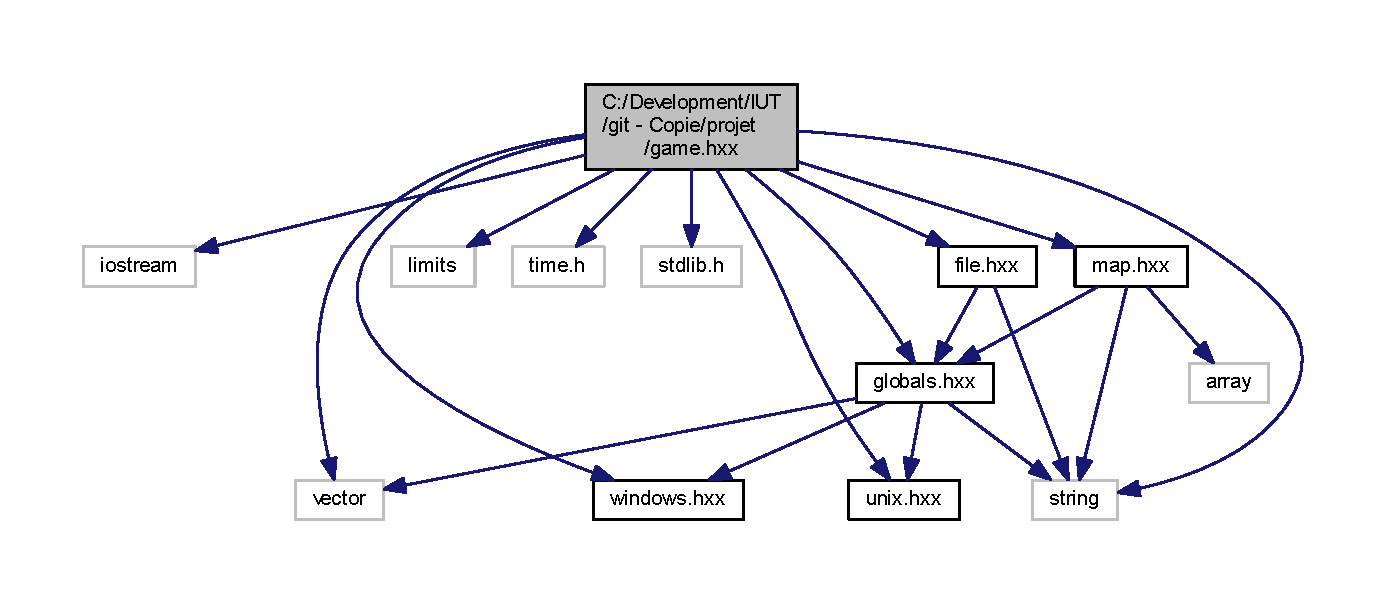
\includegraphics[width=350pt]{game_8hxx__incl}
\end{center}
\end{figure}
This graph shows which files directly or indirectly include this file\-:\nopagebreak
\begin{figure}[H]
\begin{center}
\leavevmode
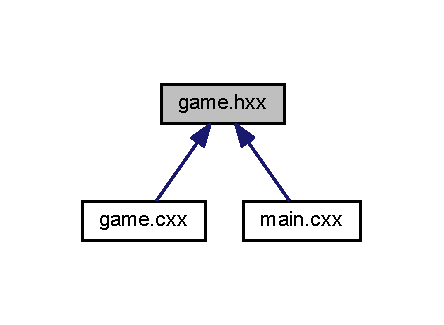
\includegraphics[width=182pt]{game_8hxx__dep__incl}
\end{center}
\end{figure}
\subsection*{Namespaces}
\begin{DoxyCompactItemize}
\item 
\hyperlink{namespace_chase_game}{Chase\-Game}
\begin{DoxyCompactList}\small\item\em Main namespace Project namespace for the game Contains all the funcitons, structs, enums and constansts related to the game. \end{DoxyCompactList}\end{DoxyCompactItemize}
\subsection*{Macros}
\begin{DoxyCompactItemize}
\item 
\#define \hyperlink{game_8hxx_aa3cda2fe747b6350757b7ced1c976ae3}{game\-\_\-h}
\end{DoxyCompactItemize}
\subsection*{Functions}
\begin{DoxyCompactItemize}
\item 
char \hyperlink{namespace_chase_game_ab5112517855da810fe3b7bdb81d58484}{Chase\-Game\-::\-Process\-Input} (C\-Matrix \&Mat, const char Input, S\-Game\-Status \&Config)
\begin{DoxyCompactList}\small\item\em Processes user input. \end{DoxyCompactList}\item 
bool \hyperlink{namespace_chase_game_a978204f0ec269a6fa5f43bb523d84e57}{Chase\-Game\-::\-Game\-Loop} (C\-Matrix \&Mat, S\-Map\-Gen\-Params \&Map\-Gen\-Params, S\-Game\-Status \&Config, map$<$ string, sf\-::\-Music \& $>$ \&Music)
\begin{DoxyCompactList}\small\item\em This is the game loop. \end{DoxyCompactList}\item 
void \hyperlink{namespace_chase_game_a528073d13296b3cf84a6ae07c3550e74}{Chase\-Game\-::\-Start\-Game} ()
\begin{DoxyCompactList}\small\item\em This function starts the game. \end{DoxyCompactList}\item 
void \hyperlink{namespace_chase_game_a4b28a3a3594d145b0ce1d1bf179e88a3}{Chase\-Game\-::\-Store\-Char\-History} (const char Input, S\-Game\-Status \&Game\-Status)
\begin{DoxyCompactList}\small\item\em Stores last 6 inputs. \end{DoxyCompactList}\end{DoxyCompactItemize}


\subsection{Detailed Description}
\hyperlink{game_8cxx}{game.\-cxx} function prototypes \begin{DoxyAuthor}{Author}

\end{DoxyAuthor}
\begin{DoxyDate}{Date}
09/01/14 
\end{DoxyDate}
\begin{DoxyVersion}{Version}
1 
\end{DoxyVersion}


Definition in file \hyperlink{game_8hxx_source}{game.\-hxx}.



\subsection{Macro Definition Documentation}
\hypertarget{game_8hxx_aa3cda2fe747b6350757b7ced1c976ae3}{\index{game.\-hxx@{game.\-hxx}!game\-\_\-h@{game\-\_\-h}}
\index{game\-\_\-h@{game\-\_\-h}!game.hxx@{game.\-hxx}}
\subsubsection[{game\-\_\-h}]{\setlength{\rightskip}{0pt plus 5cm}\#define game\-\_\-h}}\label{game_8hxx_aa3cda2fe747b6350757b7ced1c976ae3}


Definition at line 25 of file game.\-hxx.


\hypertarget{globals_8hxx}{\section{globals.\-hxx File Reference}
\label{globals_8hxx}\index{globals.\-hxx@{globals.\-hxx}}
}


Defines global constants and variables for the \hyperlink{namespace_chase_game}{Chase\-Game} namespace.  


{\ttfamily \#include \char`\"{}unix.\-hxx\char`\"{}}\\*
{\ttfamily \#include $<$vector$>$}\\*
{\ttfamily \#include $<$string$>$}\\*
Include dependency graph for globals.\-hxx\-:\nopagebreak
\begin{figure}[H]
\begin{center}
\leavevmode
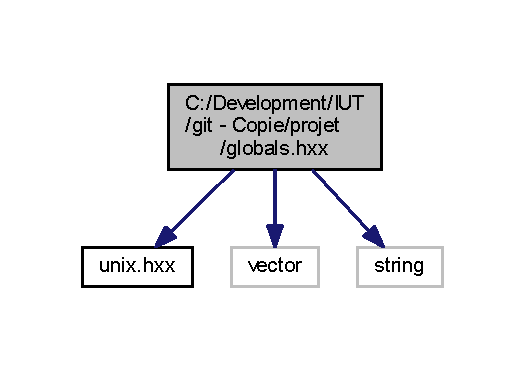
\includegraphics[width=252pt]{globals_8hxx__incl}
\end{center}
\end{figure}
This graph shows which files directly or indirectly include this file\-:\nopagebreak
\begin{figure}[H]
\begin{center}
\leavevmode
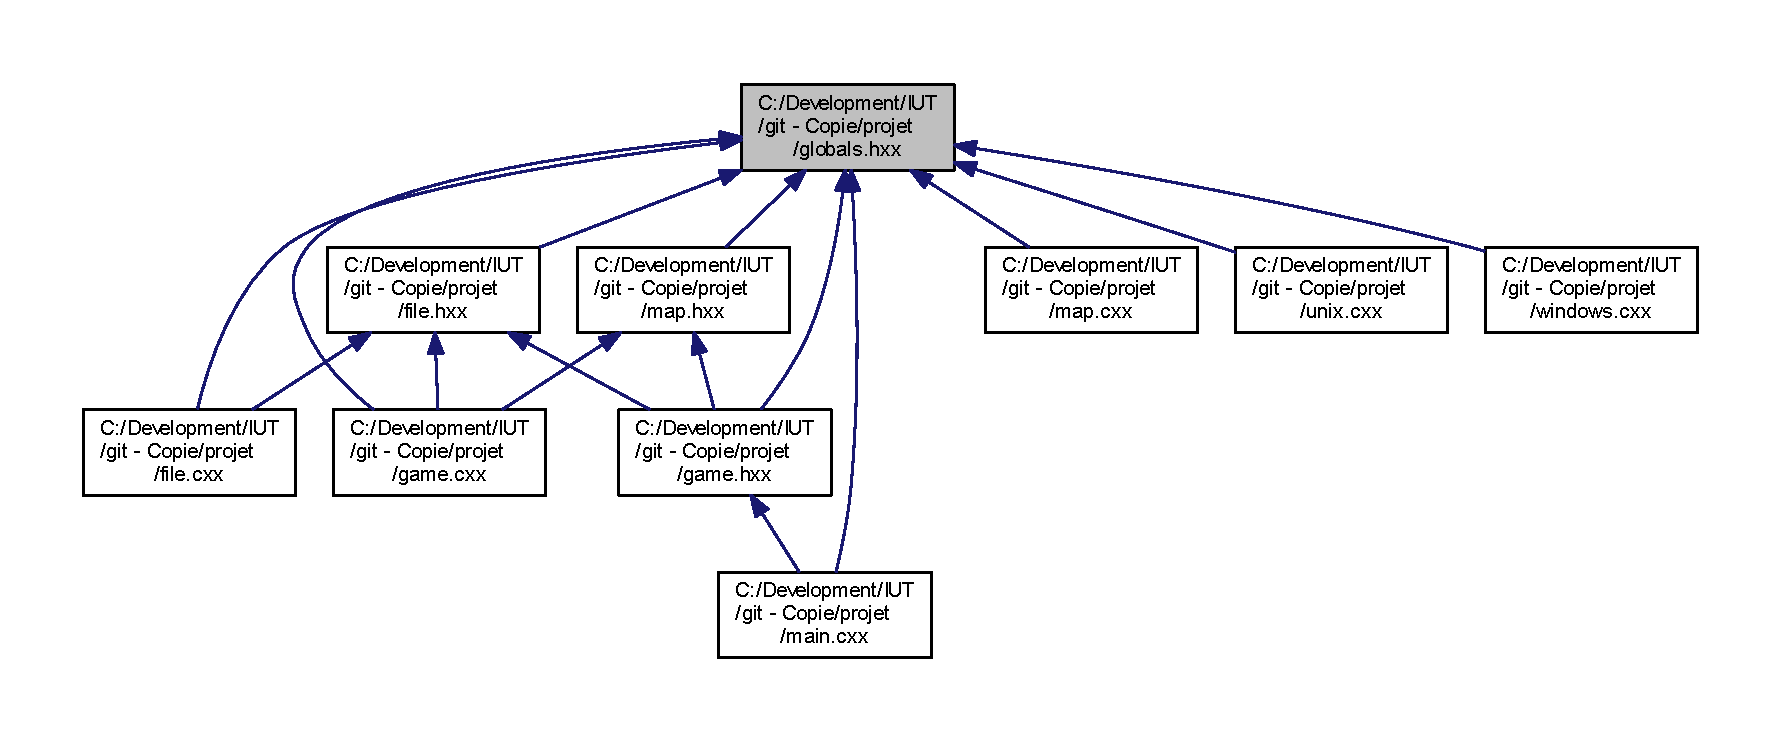
\includegraphics[width=350pt]{globals_8hxx__dep__incl}
\end{center}
\end{figure}
\subsection*{Classes}
\begin{DoxyCompactItemize}
\item 
struct \hyperlink{struct_chase_game_1_1_s_player_pos}{Chase\-Game\-::\-S\-Player\-Pos}
\begin{DoxyCompactList}\small\item\em Defines a position. \end{DoxyCompactList}\item 
struct \hyperlink{struct_chase_game_1_1_s_map_gen_params}{Chase\-Game\-::\-S\-Map\-Gen\-Params}
\begin{DoxyCompactList}\small\item\em Contains all the map generation parameters. \end{DoxyCompactList}\item 
struct \hyperlink{struct_chase_game_1_1_s_player_keys}{Chase\-Game\-::\-S\-Player\-Keys}
\begin{DoxyCompactList}\small\item\em Player specific keys. \end{DoxyCompactList}\item 
struct \hyperlink{struct_chase_game_1_1_s_player_state}{Chase\-Game\-::\-S\-Player\-State}
\begin{DoxyCompactList}\small\item\em Player state. \end{DoxyCompactList}\item 
struct \hyperlink{struct_chase_game_1_1_s_color_set}{Chase\-Game\-::\-S\-Color\-Set}
\begin{DoxyCompactList}\small\item\em Color set to use when displaying the map. \end{DoxyCompactList}\item 
struct \hyperlink{struct_chase_game_1_1_s_lang_strings}{Chase\-Game\-::\-S\-Lang\-Strings}
\begin{DoxyCompactList}\small\item\em Localised strings. \end{DoxyCompactList}\item 
struct \hyperlink{struct_chase_game_1_1_s_game_status}{Chase\-Game\-::\-S\-Game\-Status}
\begin{DoxyCompactList}\small\item\em Contains game configuration. \end{DoxyCompactList}\end{DoxyCompactItemize}
\subsection*{Namespaces}
\begin{DoxyCompactItemize}
\item 
\hyperlink{namespace_chase_game}{Chase\-Game}
\begin{DoxyCompactList}\small\item\em Main namespace Project namespace for the game Contains all the funcitons, structs, enums and constansts related to the game. \end{DoxyCompactList}\end{DoxyCompactItemize}
\subsection*{Typedefs}
\begin{DoxyCompactItemize}
\item 
typedef std\-::vector$<$ char $>$ \hyperlink{namespace_chase_game_aa09cf1806d3b1f59d36cfabadeaca6a2}{Chase\-Game\-::\-C\-V\-Line}
\begin{DoxyCompactList}\small\item\em Matrix line type. \end{DoxyCompactList}\item 
typedef std\-::vector$<$ C\-V\-Line $>$ \hyperlink{namespace_chase_game_a469449f9237e59efce3982127366c550}{Chase\-Game\-::\-C\-Matrix}
\begin{DoxyCompactList}\small\item\em Matrix type. \end{DoxyCompactList}\end{DoxyCompactItemize}
\subsection*{Enumerations}
\begin{DoxyCompactItemize}
\item 
enum \hyperlink{namespace_chase_game_a2501a45afa3eb11b10e04d79a8349796}{Chase\-Game\-::\-Langs} \{ \hyperlink{namespace_chase_game_a2501a45afa3eb11b10e04d79a8349796a4259ad53ebc5f91f2615cf5a5f59bece}{Chase\-Game\-::\-L\-A\-N\-G\-\_\-\-F\-R}, 
\hyperlink{namespace_chase_game_a2501a45afa3eb11b10e04d79a8349796a8d86c92b659a6ebac045d0a20e3fba0d}{Chase\-Game\-::\-L\-A\-N\-G\-\_\-\-E\-N}, 
\hyperlink{namespace_chase_game_a2501a45afa3eb11b10e04d79a8349796a2458ded06b17611b5fb00d6a095a4dd2}{Chase\-Game\-::\-L\-A\-N\-G\-\_\-\-E\-S}
 \}
\begin{DoxyCompactList}\small\item\em Language codes. \end{DoxyCompactList}\item 
enum \hyperlink{namespace_chase_game_a5d785ea23167a3b7e44e045097cd457e}{Chase\-Game\-::\-Difficulty\-Levels} \{ \hyperlink{namespace_chase_game_a5d785ea23167a3b7e44e045097cd457ea8511737cb33e0a6022084ed1b5c05092}{Chase\-Game\-::\-D\-I\-F\-F\-L\-V\-L\-\_\-\-E\-A\-S\-Y} =0, 
\hyperlink{namespace_chase_game_a5d785ea23167a3b7e44e045097cd457ea124bdf49731fecdaa92d39fbd9d98f26}{Chase\-Game\-::\-D\-I\-F\-F\-L\-V\-L\-\_\-\-N\-O\-R\-M} =1, 
\hyperlink{namespace_chase_game_a5d785ea23167a3b7e44e045097cd457ea67fccff53bbaeaa47737530842f5c4f5}{Chase\-Game\-::\-D\-I\-F\-F\-L\-V\-L\-\_\-\-H\-A\-R\-D} =2, 
\hyperlink{namespace_chase_game_a5d785ea23167a3b7e44e045097cd457ea6c71b45deb89801d0e11e674d21e3e51}{Chase\-Game\-::\-D\-I\-F\-F\-L\-V\-L\-\_\-\-C\-R\-Z\-Y} =3
 \}
\begin{DoxyCompactList}\small\item\em Difficulty levels. \end{DoxyCompactList}\item 
enum \hyperlink{namespace_chase_game_a5acdf639e912d1e78814b7fae21afc7b}{Chase\-Game\-::\-Console\-Colors} \{ \\*
\hyperlink{namespace_chase_game_a5acdf639e912d1e78814b7fae21afc7ba7c17af5d1ff079f2a505dd61f9e1ddae}{Chase\-Game\-::\-C\-L\-R\-\_\-\-B\-L\-A\-C\-K} =30, 
\hyperlink{namespace_chase_game_a5acdf639e912d1e78814b7fae21afc7baea24ff932a53ca9fd904e2b607407c0a}{Chase\-Game\-::\-C\-L\-R\-\_\-\-R\-E\-D} =31, 
\hyperlink{namespace_chase_game_a5acdf639e912d1e78814b7fae21afc7ba9f550f868a825b9a3be5a7d0dbcc4852}{Chase\-Game\-::\-C\-L\-R\-\_\-\-G\-R\-E\-E\-N} =32, 
\hyperlink{namespace_chase_game_a5acdf639e912d1e78814b7fae21afc7ba9ac15128d0c53aad431c8d1da78cf17a}{Chase\-Game\-::\-C\-L\-R\-\_\-\-Y\-E\-L\-L\-O\-W} =33, 
\\*
\hyperlink{namespace_chase_game_a5acdf639e912d1e78814b7fae21afc7ba206cb9e67be830b771bbf44488c40d66}{Chase\-Game\-::\-C\-L\-R\-\_\-\-B\-L\-U\-E} =34, 
\hyperlink{namespace_chase_game_a5acdf639e912d1e78814b7fae21afc7ba6ce8de58df1a149d734ebcdbf711fed9}{Chase\-Game\-::\-C\-L\-R\-\_\-\-M\-A\-G\-E\-N\-T\-A} =35, 
\hyperlink{namespace_chase_game_a5acdf639e912d1e78814b7fae21afc7baa190fadb3645da6bca096b377cda2542}{Chase\-Game\-::\-C\-L\-R\-\_\-\-C\-Y\-A\-N} =36, 
\hyperlink{namespace_chase_game_a5acdf639e912d1e78814b7fae21afc7baefa8ce8fa562fcb596842176d5b1222d}{Chase\-Game\-::\-C\-L\-R\-\_\-\-W\-H\-I\-T\-E} =37, 
\\*
\hyperlink{namespace_chase_game_a5acdf639e912d1e78814b7fae21afc7ba1d11a3c17a5e12280a482d5d39c12f09}{Chase\-Game\-::\-C\-L\-R\-\_\-\-G\-R\-E\-Y} =30, 
\hyperlink{namespace_chase_game_a5acdf639e912d1e78814b7fae21afc7bab062e50df9f6e90f6c4cce85d5d420df}{Chase\-Game\-::\-C\-L\-R\-\_\-\-R\-E\-S\-E\-T} =0
 \}
\begin{DoxyCompactList}\small\item\em Unix color values. \end{DoxyCompactList}\item 
enum \hyperlink{namespace_chase_game_a85936e0bdb5509ede7ebb2543de5be42}{Chase\-Game\-::\-Game\-Music\-State} \{ \hyperlink{namespace_chase_game_a85936e0bdb5509ede7ebb2543de5be42ae2cef0894718493a1e334a948734fe65}{Chase\-Game\-::\-G\-M\-S\-\_\-\-T\-I\-T\-L\-E}, 
\hyperlink{namespace_chase_game_a85936e0bdb5509ede7ebb2543de5be42a9c9cc6c997ce9d50efd2f3d815323b11}{Chase\-Game\-::\-G\-M\-S\-\_\-\-S\-T\-A\-R\-T\-I\-N\-G}, 
\hyperlink{namespace_chase_game_a85936e0bdb5509ede7ebb2543de5be42a575913ea08f1bd0667c644624b56102f}{Chase\-Game\-::\-G\-M\-S\-\_\-\-I\-N\-G\-A\-M\-E}, 
\hyperlink{namespace_chase_game_a85936e0bdb5509ede7ebb2543de5be42aeff71e80a88a58ab6f8d049daaccc84a}{Chase\-Game\-::\-G\-M\-S\-\_\-\-S\-T\-O\-P}
 \}
\begin{DoxyCompactList}\small\item\em Music state, the value changes the music tracks being played. \end{DoxyCompactList}\end{DoxyCompactItemize}
\subsection*{Variables}
\begin{DoxyCompactItemize}
\item 
const char \hyperlink{namespace_chase_game_a8452e2d6de618e4ca7a9f76b082b52a4}{Chase\-Game\-::\-K\-Token\-Player1} = 'X'
\begin{DoxyCompactList}\small\item\em Character representing player one. \end{DoxyCompactList}\item 
const char \hyperlink{namespace_chase_game_ae27343407c21a8d6e3cf26b736bd5527}{Chase\-Game\-::\-K\-Token\-Player2} = 'O'
\begin{DoxyCompactList}\small\item\em Character representing player two. \end{DoxyCompactList}\item 
const char \hyperlink{namespace_chase_game_aa036d4de40188ba2e1aa36ab6cfaf1da}{Chase\-Game\-::\-K\-Empty} = ' '
\begin{DoxyCompactList}\small\item\em Character representing voidness. \end{DoxyCompactList}\item 
const char \hyperlink{namespace_chase_game_ad86181b2050b912dab9d69d2f0bea76e}{Chase\-Game\-::\-K\-Obstacle} = '\#'
\begin{DoxyCompactList}\small\item\em Character representing obstacles and walls. \end{DoxyCompactList}\item 
const char \hyperlink{namespace_chase_game_a12d6411bb9a72150acba6060bb1587e1}{Chase\-Game\-::\-K\-Cancelled} = '0'
\begin{DoxyCompactList}\small\item\em Character sent when a move is not allowed. \end{DoxyCompactList}\item 
const char \hyperlink{namespace_chase_game_a1f787138e31b0a9dc2fbaad3547b246a}{Chase\-Game\-::\-K\-Exit} = 'Q'
\begin{DoxyCompactList}\small\item\em Character sent when the user wants to exit the game (escape) \end{DoxyCompactList}\item 
const char \hyperlink{namespace_chase_game_a202a236c81f69bdfc031abd6654b8132}{Chase\-Game\-::\-K\-Bonus} = '@'
\begin{DoxyCompactList}\small\item\em Character representing bonuses. \end{DoxyCompactList}\item 
const char \hyperlink{namespace_chase_game_ad3c85aebf9881b576634247b5db00b96}{Chase\-Game\-::\-K\-Malus} = '\$'
\begin{DoxyCompactList}\small\item\em Character representing maluses. \end{DoxyCompactList}\end{DoxyCompactItemize}


\subsection{Detailed Description}
Defines global constants and variables for the \hyperlink{namespace_chase_game}{Chase\-Game} namespace. \begin{DoxyAuthor}{Author}
Josua Gonzalez 
\end{DoxyAuthor}
\begin{DoxyDate}{Date}
07/01/14 
\end{DoxyDate}
\begin{DoxyVersion}{Version}
1
\end{DoxyVersion}
Contains constants and structs used in the game code 
\hypertarget{main_8cxx}{\section{C\-:/\-Development/\-I\-U\-T/git -\/ Copie/projet/main.cxx File Reference}
\label{main_8cxx}\index{C\-:/\-Development/\-I\-U\-T/git -\/ Copie/projet/main.\-cxx@{C\-:/\-Development/\-I\-U\-T/git -\/ Copie/projet/main.\-cxx}}
}


Main file.  


{\ttfamily \#include $<$time.\-h$>$}\\*
{\ttfamily \#include $<$stdlib.\-h$>$}\\*
{\ttfamily \#include \char`\"{}globals.\-hxx\char`\"{}}\\*
{\ttfamily \#include \char`\"{}game.\-hxx\char`\"{}}\\*
Include dependency graph for main.\-cxx\-:\nopagebreak
\begin{figure}[H]
\begin{center}
\leavevmode
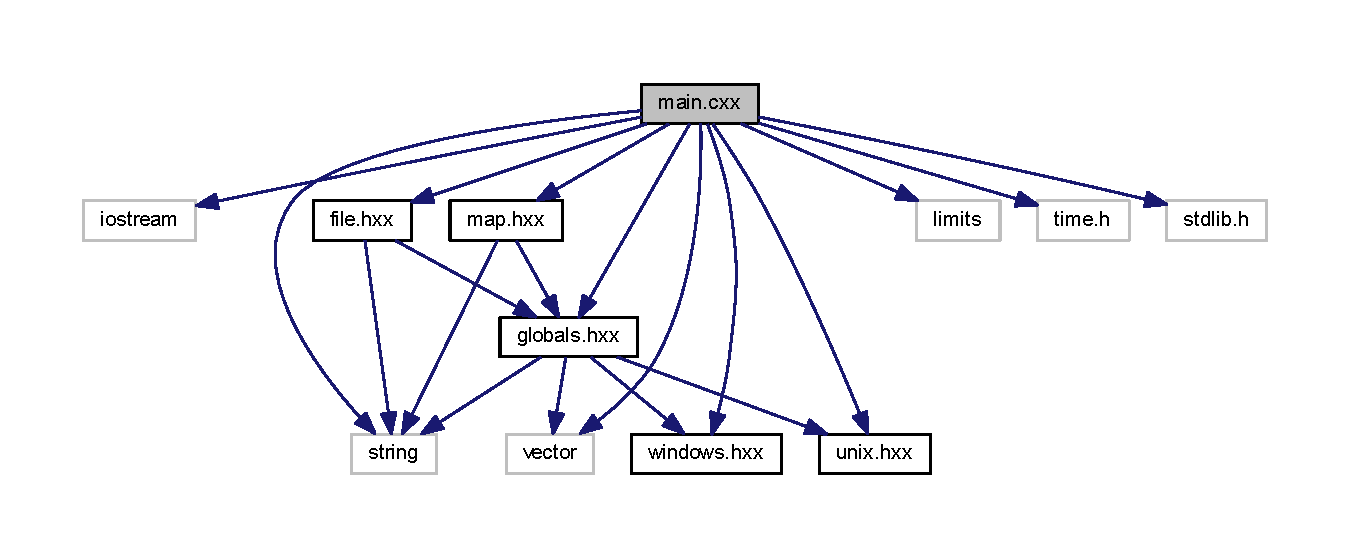
\includegraphics[width=350pt]{main_8cxx__incl}
\end{center}
\end{figure}
\subsection*{Functions}
\begin{DoxyCompactItemize}
\item 
int \hyperlink{main_8cxx_ae66f6b31b5ad750f1fe042a706a4e3d4}{main} ()
\begin{DoxyCompactList}\small\item\em Program main, the program does not accept arguments. \end{DoxyCompactList}\end{DoxyCompactItemize}


\subsection{Detailed Description}
Main file. \begin{DoxyAuthor}{Author}
Josua Gonzalez 
\end{DoxyAuthor}
\begin{DoxyDate}{Date}
17/12/13 
\end{DoxyDate}
\begin{DoxyVersion}{Version}
1 
\end{DoxyVersion}


Definition in file \hyperlink{main_8cxx_source}{main.\-cxx}.



\subsection{Function Documentation}
\hypertarget{main_8cxx_ae66f6b31b5ad750f1fe042a706a4e3d4}{\index{main.\-cxx@{main.\-cxx}!main@{main}}
\index{main@{main}!main.cxx@{main.\-cxx}}
\subsubsection[{main}]{\setlength{\rightskip}{0pt plus 5cm}int main (
\begin{DoxyParamCaption}
{}
\end{DoxyParamCaption}
)}}\label{main_8cxx_ae66f6b31b5ad750f1fe042a706a4e3d4}


Program main, the program does not accept arguments. 

\begin{DoxyReturn}{Returns}
0 
\end{DoxyReturn}


Definition at line 33 of file main.\-cxx.



Here is the call graph for this function\-:\nopagebreak
\begin{figure}[H]
\begin{center}
\leavevmode
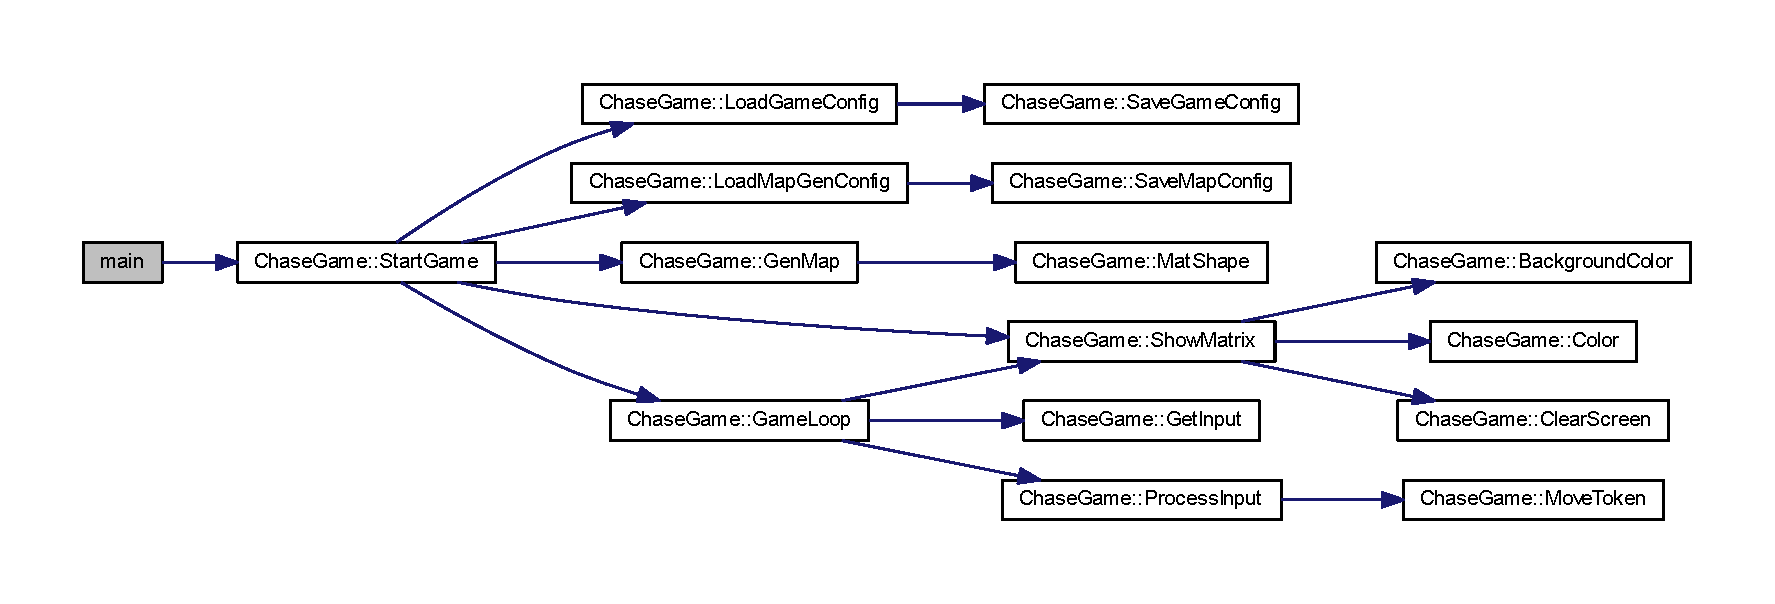
\includegraphics[width=350pt]{main_8cxx_ae66f6b31b5ad750f1fe042a706a4e3d4_cgraph}
\end{center}
\end{figure}



\hypertarget{map_8cxx}{\section{C\-:/\-Development/\-I\-U\-T/git -\/ Copie/projet/map.cxx File Reference}
\label{map_8cxx}\index{C\-:/\-Development/\-I\-U\-T/git -\/ Copie/projet/map.\-cxx@{C\-:/\-Development/\-I\-U\-T/git -\/ Copie/projet/map.\-cxx}}
}


Map related function.  


{\ttfamily \#include $<$iostream$>$}\\*
{\ttfamily \#include $<$fstream$>$}\\*
{\ttfamily \#include $<$string$>$}\\*
{\ttfamily \#include $<$vector$>$}\\*
{\ttfamily \#include $<$array$>$}\\*
{\ttfamily \#include \char`\"{}globals.\-hxx\char`\"{}}\\*
{\ttfamily \#include \char`\"{}windows.\-hxx\char`\"{}}\\*
{\ttfamily \#include \char`\"{}unix.\-hxx\char`\"{}}\\*
{\ttfamily \#include \char`\"{}map.\-hxx\char`\"{}}\\*
Include dependency graph for map.\-cxx\-:\nopagebreak
\begin{figure}[H]
\begin{center}
\leavevmode
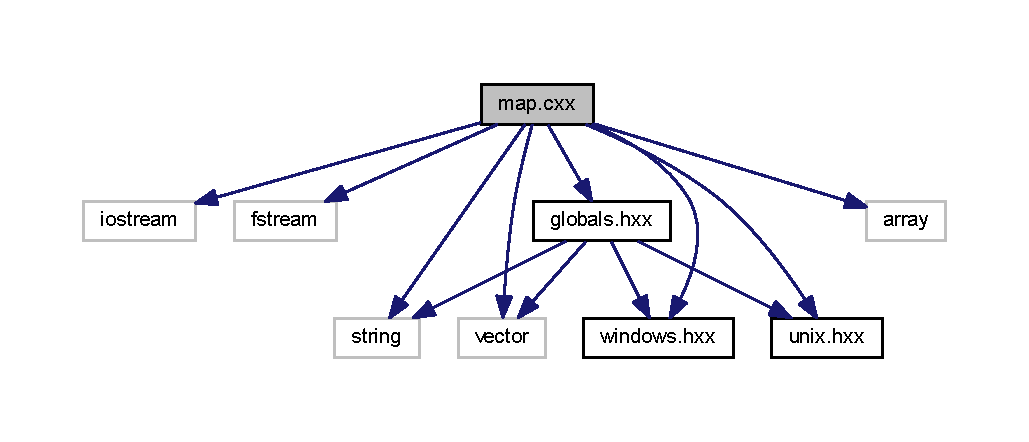
\includegraphics[width=350pt]{map_8cxx__incl}
\end{center}
\end{figure}
\subsection*{Namespaces}
\begin{DoxyCompactItemize}
\item 
\hyperlink{namespace_chase_game}{Chase\-Game}
\end{DoxyCompactItemize}
\subsection*{Functions}
\begin{DoxyCompactItemize}
\item 
void \hyperlink{namespace_chase_game_ac12626138d0e2c49669eba73ffb4e4b7}{Chase\-Game\-::\-Mat\-Shape} (C\-Matrix \&Mat, const array$<$ bool, 9 $>$ Tab, const unsigned Y, const unsigned X)
\item 
void \hyperlink{namespace_chase_game_a15617c8a111cd66bf5d24fd1e82a119d}{Chase\-Game\-::\-Gen\-Map} (C\-Matrix \&Mat, const S\-Map\-Gen\-Params \&Params, const int Difficulty)
\begin{DoxyCompactList}\small\item\em Creates game matrix from the parameters and config file. \end{DoxyCompactList}\item 
char \hyperlink{namespace_chase_game_a1dfe4bdbd50ee18cf85760219ea90b03}{Chase\-Game\-::\-Move\-Token} (C\-Matrix \&Mat, const char Move, S\-Player\-Pos \&Pos, const S\-Player\-Keys \&Key\-Codes)
\begin{DoxyCompactList}\small\item\em Move a token in the game matrix. \end{DoxyCompactList}\item 
void \hyperlink{namespace_chase_game_a871395f1f12e55eaa3d341b8ef2cbb78}{Chase\-Game\-::\-Show\-Matrix} (const C\-Matrix \&Mat, const S\-Color\-Set \&Color\-Set)
\begin{DoxyCompactList}\small\item\em Displays game matrix. \end{DoxyCompactList}\end{DoxyCompactItemize}


\subsection{Detailed Description}
Map related function. \begin{DoxyAuthor}{Author}

\end{DoxyAuthor}
\begin{DoxyDate}{Date}
08/01/14 
\end{DoxyDate}
\begin{DoxyVersion}{Version}
1
\end{DoxyVersion}
Contains functions that generate the map, displays it, move tokens and other related functions. 

Definition in file \hyperlink{map_8cxx_source}{map.\-cxx}.


\hypertarget{map_8hxx}{\section{map.\-hxx File Reference}
\label{map_8hxx}\index{map.\-hxx@{map.\-hxx}}
}


\hyperlink{map_8cxx}{map.\-cxx} function prototypes  


{\ttfamily \#include $<$string$>$}\\*
{\ttfamily \#include $<$array$>$}\\*
{\ttfamily \#include \char`\"{}globals.\-hxx\char`\"{}}\\*
Include dependency graph for map.\-hxx\-:
\nopagebreak
\begin{figure}[H]
\begin{center}
\leavevmode
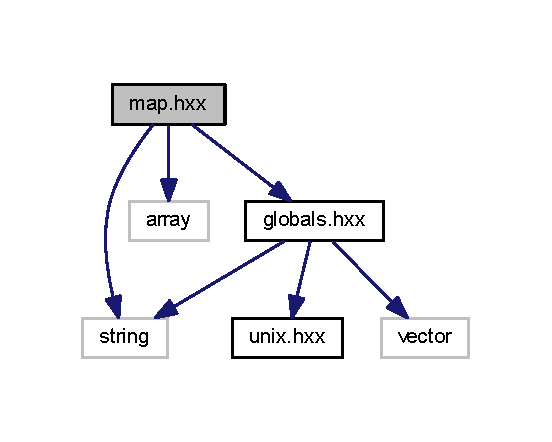
\includegraphics[width=265pt]{map_8hxx__incl}
\end{center}
\end{figure}
This graph shows which files directly or indirectly include this file\-:
\nopagebreak
\begin{figure}[H]
\begin{center}
\leavevmode
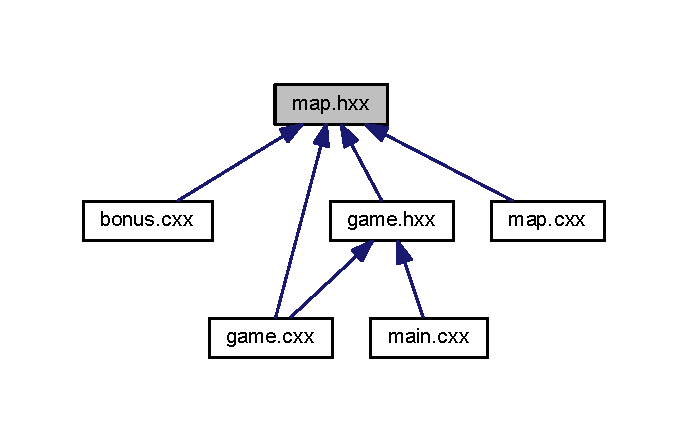
\includegraphics[width=330pt]{map_8hxx__dep__incl}
\end{center}
\end{figure}
\subsection*{Namespaces}
\begin{DoxyCompactItemize}
\item 
\hyperlink{namespace_chase_game}{Chase\-Game}
\begin{DoxyCompactList}\small\item\em Main namespace Project namespace for the game Contains all the funcitons, structs, enums and constansts related to the game. \end{DoxyCompactList}\end{DoxyCompactItemize}
\subsection*{Functions}
\begin{DoxyCompactItemize}
\item 
void \hyperlink{namespace_chase_game_a049d8d8beb22431889ca7ba34cc90871}{Chase\-Game\-::\-Mat\-Shape} (C\-Matrix \&Mat, const std\-::array$<$ bool, 9 $>$ Tab, const unsigned Y, const unsigned X)
\begin{DoxyCompactList}\small\item\em Generate a random shape in the map. \end{DoxyCompactList}\item 
void \hyperlink{namespace_chase_game_a15617c8a111cd66bf5d24fd1e82a119d}{Chase\-Game\-::\-Gen\-Map} (C\-Matrix \&Mat, const S\-Map\-Gen\-Params \&Params, const int Difficulty)
\begin{DoxyCompactList}\small\item\em Creates game matrix from the parameters and config file. \end{DoxyCompactList}\item 
void \hyperlink{namespace_chase_game_a871395f1f12e55eaa3d341b8ef2cbb78}{Chase\-Game\-::\-Show\-Matrix} (const C\-Matrix \&Mat, const S\-Color\-Set \&Color\-Set)
\begin{DoxyCompactList}\small\item\em Displays game matrix. \end{DoxyCompactList}\item 
char \hyperlink{namespace_chase_game_a1dfe4bdbd50ee18cf85760219ea90b03}{Chase\-Game\-::\-Move\-Token} (C\-Matrix \&Mat, const char Move, S\-Player\-Pos \&Pos, const S\-Player\-Keys \&Key\-Codes)
\begin{DoxyCompactList}\small\item\em Move a token in the game matrix. \end{DoxyCompactList}\item 
unsigned \hyperlink{namespace_chase_game_aee2df7cbf4974e167612a7415943f3b0}{Chase\-Game\-::\-R\-Rand} (unsigned Min, unsigned Max)
\item 
void \hyperlink{namespace_chase_game_a6351b2bdc824272990926fbb8e8ad359}{Chase\-Game\-::\-Gen\-Bonus\-Malus} (C\-Matrix \&Mat)
\begin{DoxyCompactList}\small\item\em Display bonus. \end{DoxyCompactList}\end{DoxyCompactItemize}


\subsection{Detailed Description}
\hyperlink{map_8cxx}{map.\-cxx} function prototypes \begin{DoxyAuthor}{Author}

\end{DoxyAuthor}
\begin{DoxyDate}{Date}
08/01/14 
\end{DoxyDate}
\begin{DoxyVersion}{Version}
1 
\end{DoxyVersion}

\hypertarget{_r_e_a_d_m_e_8md}{\section{C\-:/\-Development/\-I\-U\-T/git -\/ Copie/projet/\-R\-E\-A\-D\-M\-E.md File Reference}
\label{_r_e_a_d_m_e_8md}\index{C\-:/\-Development/\-I\-U\-T/git -\/ Copie/projet/\-R\-E\-A\-D\-M\-E.\-md@{C\-:/\-Development/\-I\-U\-T/git -\/ Copie/projet/\-R\-E\-A\-D\-M\-E.\-md}}
}

\hypertarget{unix_8cxx}{\section{C\-:/\-Development/\-I\-U\-T/git -\/ Copie/projet/unix.cxx File Reference}
\label{unix_8cxx}\index{C\-:/\-Development/\-I\-U\-T/git -\/ Copie/projet/unix.\-cxx@{C\-:/\-Development/\-I\-U\-T/git -\/ Copie/projet/unix.\-cxx}}
}


Defines unix-\/only functions.  


{\ttfamily \#include \char`\"{}globals.\-hxx\char`\"{}}\\*
{\ttfamily \#include \char`\"{}unix.\-hxx\char`\"{}}\\*
{\ttfamily \#include $<$iostream$>$}\\*
{\ttfamily \#include $<$limits$>$}\\*
{\ttfamily \#include $<$termios.\-h$>$}\\*
{\ttfamily \#include $<$unistd.\-h$>$}\\*
{\ttfamily \#include $<$stdio.\-h$>$}\\*
Include dependency graph for unix.\-cxx\-:\nopagebreak
\begin{figure}[H]
\begin{center}
\leavevmode
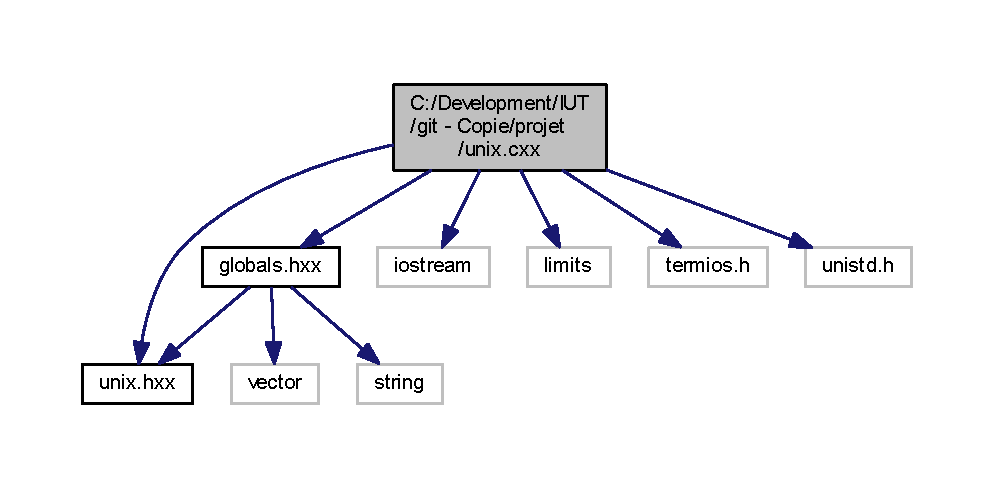
\includegraphics[width=350pt]{unix_8cxx__incl}
\end{center}
\end{figure}
\subsection*{Namespaces}
\begin{DoxyCompactItemize}
\item 
\hyperlink{namespace_chase_game}{Chase\-Game}
\begin{DoxyCompactList}\small\item\em Main namespace Project namespace for the game Contains all the funcitons, structs, enums and constansts related to the game. \end{DoxyCompactList}\end{DoxyCompactItemize}
\subsection*{Functions}
\begin{DoxyCompactItemize}
\item 
void \hyperlink{namespace_chase_game_a3a7382465f6f23fe77cde4e589fb80d6}{Chase\-Game\-::\-Clear\-Screen} ()
\begin{DoxyCompactList}\small\item\em Clears screen. \end{DoxyCompactList}\item 
void \hyperlink{namespace_chase_game_a3a120300b1e200a26fe8680a33300283}{Chase\-Game\-::\-Color} (const int \&Color)
\begin{DoxyCompactList}\small\item\em Changes text color. \end{DoxyCompactList}\item 
void \hyperlink{namespace_chase_game_ad2dbfd93f4fd5725ab396d5dfa78a0c4}{Chase\-Game\-::\-Background\-Color} (const int \&Color)
\begin{DoxyCompactList}\small\item\em Changes background color. \end{DoxyCompactList}\item 
char \hyperlink{namespace_chase_game_afa8eec677de5433e0e886da19f7e9c4a}{Chase\-Game\-::\-Get\-Input} ()
\begin{DoxyCompactList}\small\item\em Captures a character from stdin. \end{DoxyCompactList}\item 
void \hyperlink{namespace_chase_game_a8ca147721cdfaf96ee1f9c5007c27142}{Chase\-Game\-::\-Sleep} (int M\-Sec)
\begin{DoxyCompactList}\small\item\em Calls usleep. \end{DoxyCompactList}\item 
void \hyperlink{namespace_chase_game_aaaedf9429ec62c336f4324d580eec51c}{Chase\-Game\-::\-Pause} ()
\begin{DoxyCompactList}\small\item\em This function pauses the program. \end{DoxyCompactList}\end{DoxyCompactItemize}


\subsection{Detailed Description}
Defines unix-\/only functions. \begin{DoxyAuthor}{Author}
Josua Gonzalez 
\end{DoxyAuthor}
\begin{DoxyDate}{Date}
07/01/14 
\end{DoxyDate}
\begin{DoxyVersion}{Version}
1
\end{DoxyVersion}
Defines unix-\/only functions 

Definition in file \hyperlink{unix_8cxx_source}{unix.\-cxx}.


\hypertarget{unix_8hxx}{\section{C\-:/\-Development/\-I\-U\-T/git -\/ Copie/projet/unix.hxx File Reference}
\label{unix_8hxx}\index{C\-:/\-Development/\-I\-U\-T/git -\/ Copie/projet/unix.\-hxx@{C\-:/\-Development/\-I\-U\-T/git -\/ Copie/projet/unix.\-hxx}}
}


Defines U\-N\-I\-X specific functions.  


This graph shows which files directly or indirectly include this file\-:
\nopagebreak
\begin{figure}[H]
\begin{center}
\leavevmode
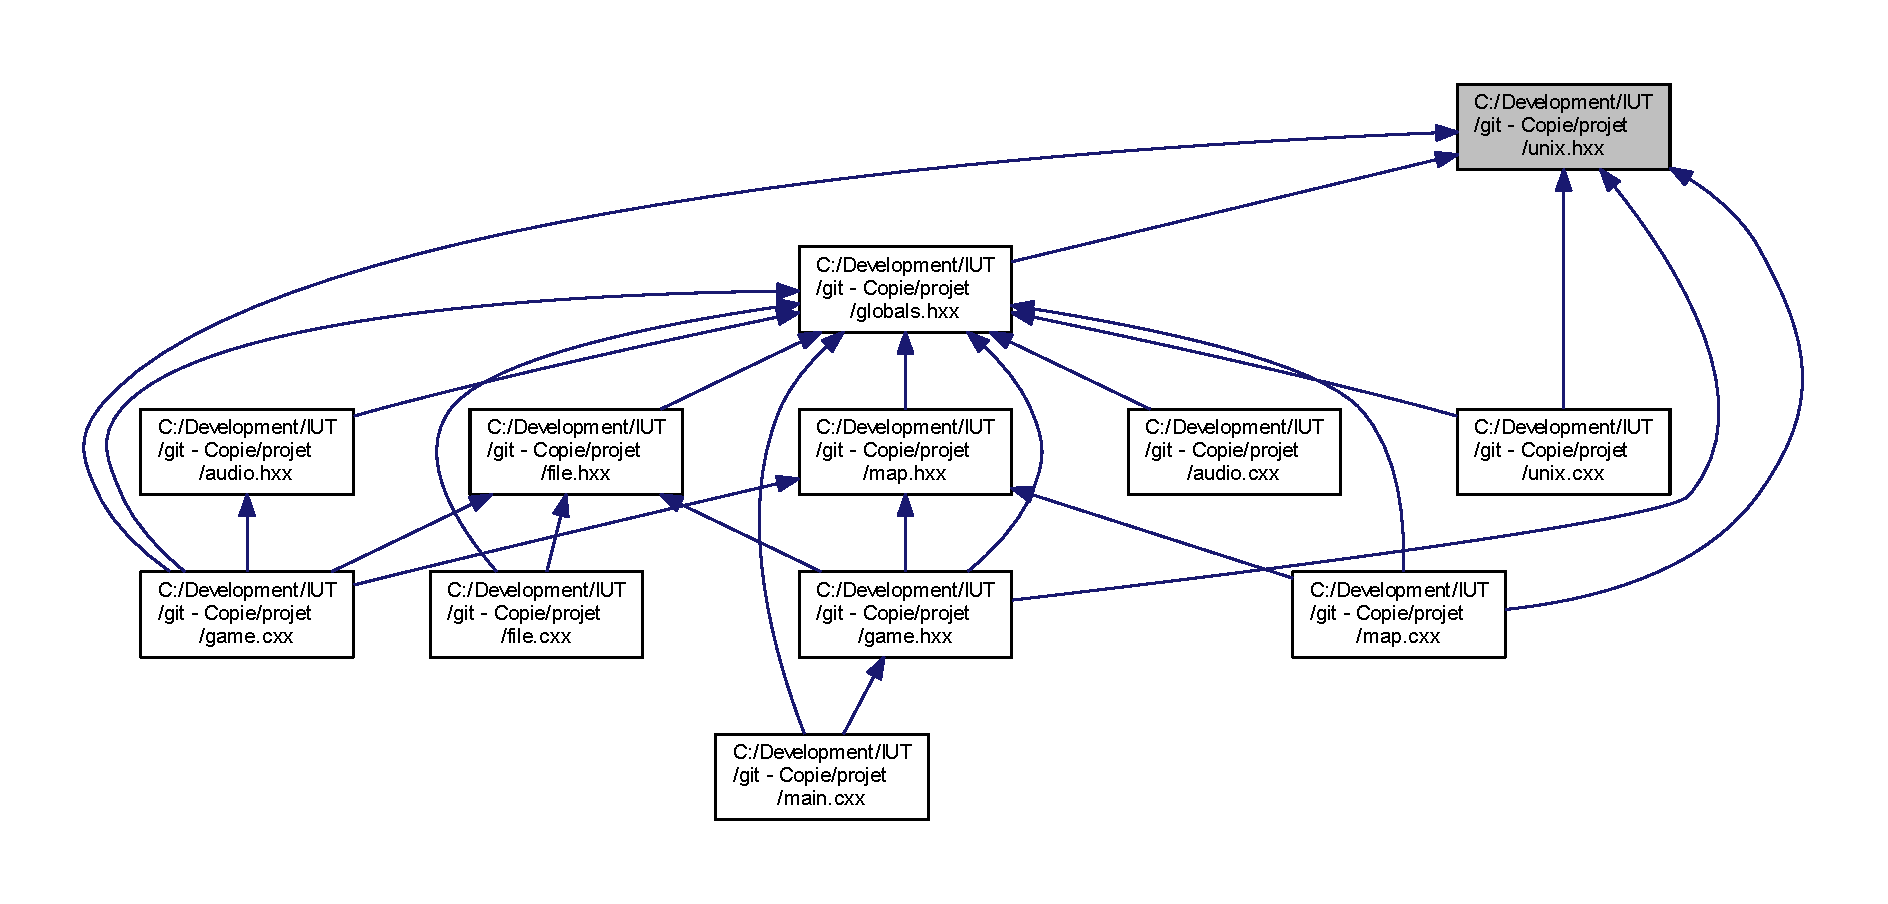
\includegraphics[width=350pt]{unix_8hxx__dep__incl}
\end{center}
\end{figure}
\subsection*{Namespaces}
\begin{DoxyCompactItemize}
\item 
\hyperlink{namespace_chase_game}{Chase\-Game}
\end{DoxyCompactItemize}


\subsection{Detailed Description}
Defines U\-N\-I\-X specific functions. \begin{DoxyAuthor}{Author}

\end{DoxyAuthor}
\begin{DoxyDate}{Date}
08/01/14 
\end{DoxyDate}
\begin{DoxyVersion}{Version}
1
\end{DoxyVersion}
Defines U\-N\-I\-X specific functions 
%--- End generated contents ---

% Index
\newpage
\phantomsection
\addcontentsline{toc}{chapter}{Index}
\printindex

\end{document}
